%
% ---------------------------------------------------------------------------------------
% VALOR T2K 5 sample nuebar appearance analysis, Run 1-9c with Run 1-9d update
% ---------------------------------------------------------------------------------------
%
\documentclass[11pt]{elsarticle}

\makeatletter
\def\ps@pprintTitle{%
 \let\@oddhead\@empty
 \let\@evenhead\@empty
 \def\@oddfoot{\centerline{\thepage}}%
 \let\@evenfoot\@oddfoot}
\makeatother

\usepackage{adjustbox}
\usepackage[toc,page]{appendix}       	% Appendix
\usepackage{amsfonts}                 	% Extra symbols
\usepackage{amsmath}
\usepackage{appendix}
\usepackage{booktabs}
\usepackage{caption}					% Use when minipaging figures & tables together
\usepackage{color}
\usepackage{dcolumn}					% align table columns on decimal point
\usepackage[figuresright]{rotating}		% if you have landscape tables
\usepackage{float}
\usepackage[margin=2.50cm]{geometry}  	% Tweak margins
\usepackage{graphicx}                 	% PostScript figures
\usepackage{hyperref} 					% Linkable contents and reference without colour
\usepackage{lineno}                   	% For printing the line numbers
\usepackage{listings}
\usepackage{longtable}
\usepackage{multirow}                 	% Fancy tables
\usepackage{natbib}                   	% For building bibliography with \cite{}
\usepackage{pdflscape}                  % allow page to be landscape for large tables
\usepackage{rotate}                     % rotate text in tables
\usepackage{siunitx}					% Easier units exponentials etc
\usepackage{subcaption}					% Allows use of subfigure
\usepackage[table,dvipsnames]{xcolor}	% Fancy tables and colors
\usepackage{xspace}		        		% Appropriate insertion of spaces after commands
\usepackage{cleveref}                   % Load after the hyperref package
\usepackage{pdflscape}
\usepackage{setspace}
\usepackage{color,soul}   				% For highlighting with \hl{}
\onehalfspacing
\DeclareSIUnit\POT{POT}

\usepackage{placeins}					% For float barriers

%\let\Oldsection\section
%\renewcommand{\section}{\FloatBarrier\Oldsection}

%\let\Oldsubsection\subsection
%\renewcommand{\subsection}{\FloatBarrier\Oldsubsection}

%\let\Oldsubsubsection\subsubsection
%\renewcommand{\subsubsection}{\FloatBarrier\Oldsubsubsection}

\crefname{appsec}{Appendix}{Appendices}

% put your own definitions here:
\newcommand{\ck}{$\checkmark$}
\newcommand{\ttbs}{\char'134}


\lstset{language=C++}

% Particle aliases
\newcommand{\nue}{\nu_{e}}
\newcommand{\numu}{\nu_{\mu}}
\newcommand{\nutau}{\nu_{\tau}}
\newcommand{\nueb}{\bar{\nu}_{e}}
\newcommand{\numub}{\bar{\nu}_{\mu}}
\newcommand{\nutaub}{\bar{\nu}_{\tau}}
\newcommand{\nub}{\bar{\nu}}
\newcommand{\nua}{\nu_{\alpha}}
\newcommand{\nuab}{\bar{\nu_{\alpha}}}

\newcommand{\numuany}{\overset{(-)}{\nu}_{\mu}}
\newcommand{\nueany}{\overset{(-)}{\nu_e}}

\newcommand{\CCzeropi}{CC \( 0\pi \)}
\newcommand{\nueCConepi}{\(\nue\) CC\( 1\pi^{+} \)}
\newcommand*{\pbar}[1]{\accentset{(-)}{#1}}

% Fit variables
\newcommand{\ssqthonethree}{$\sin^2\theta_{13}$\xspace}
\newcommand{\ssqthtwothree}{$\sin^2\theta_{23}$\xspace}
\newcommand{\ssqthonetwo}{$\sin^2\theta_{12}$\xspace}
\newcommand{\deltacp}{$\delta_{CP}$\xspace}
\newcommand{\dmsqtwothree}{$\Delta m^2_{32}$\xspace}
\newcommand{\dmsqonetwo}{$\Delta m^2_{21}$\xspace}
\newcommand{\dmsqonethree}{$\Delta m^2_{13}$\xspace}

\newcommand{\RunPeriod}{Run 1-9c\xspace}

%2D fits
\newcommand{\appearance}{\deltacp vs \ssqthonethree\xspace}
\newcommand{\disappearance}{\dmsqtwothree vs \ssqthtwothree}

% By default, LaTeX doesn't like to fill more than 0.7 of a text page with tables and graphics, 
% nor does it like too many figures per page. This behaviour can be changed:
\renewcommand\floatpagefraction{.9}
\renewcommand\topfraction{.9}
\renewcommand\bottomfraction{.9}
\renewcommand\textfraction{.1}   
\setcounter{totalnumber}{50}
\setcounter{topnumber}{50}
\setcounter{bottomnumber}{50}

\makeatletter % Remove preprint footer
\def\ps@pprintTitle{%
	\let\@oddhead\@empty
	\let\@evenhead\@empty
	\def\@oddfoot{}%
	\let\@evenfoot\@oddfoot}
\makeatother

%define new fonts, smaller than tiny (for showing large covariance matrices in a page)
\makeatletter
\ifcase \@ptsize \relax% 10pt
  \newcommand{\miniscule}{\@setfontsize\miniscule{4}{5}}% \tiny: 5/6
  \newcommand{\verytiny}{\@setfontsize\miniscule{3}{4}}% \tiny: 5/6
\or% 11pt
  \newcommand{\miniscule}{\@setfontsize\miniscule{5}{6}}% \tiny: 6/7
  \newcommand{\verytiny}{\@setfontsize\miniscule{4}{5}}% \tiny: 6/7
\or% 12pt
  \newcommand{\miniscule}{\@setfontsize\miniscule{5}{6}}% \tiny: 6/7
  \newcommand{\verytiny}{\@setfontsize\miniscule{4}{5}}% \tiny: 6/7
\fi
\makeatother

\linenumbers
%\bibliographystyle{elsart-num}

\begin{document}

%Numbers used in this tech note
% This file is for numbers that appear in several different places in the technical note.
% First argument of \newcommand can only contain lower case or upper case letters.
% Numbers and other non-letter characters will cause an error.
% When using the command in the text, please add {} after it if you want a space after the number.
% If you don't add {}, there will be no space after the number.

% TODO: Update these values for run 1-10

%
% POT
%
\newcommand{\TargetFullPot}{7.8$\times$10$^{21}$}
\newcommand{\TargetFullPotNu}{7.8$\times$10$^{21}$}
\newcommand{\TargetFullPotNuBar}{7.8$\times$10$^{21}$}

\newcommand{\NumToysSmall}{10k\xspace}
\newcommand{\NumToys}{40k\xspace}
\newcommand{\NumToysLarge}{80k\xspace}

\newcommand{\NumToysRCApp}{10k\xspace}
\newcommand{\NumToysRCDisapp}{10k\xspace}
\newcommand{\NumToysRCDelta}{40k\xspace}
\newcommand{\NumToysWORCApp}{20k\xspace}
\newcommand{\NumToysWORCDisapp}{20k\xspace}
\newcommand{\NumToysWORCDelta}{80k\xspace}

%
% Number of systematics
%
% 25 FHC flux
% 25 RHC flux
% 23 Xsec
% 18 FHC SKDet FSI
% 18 RHC SKDet FSI
% Escale
% 
\newcommand{\NFluxSyst}{50\xspace}
\newcommand{\NXsecSyst}{39\xspace}
\newcommand{\NFluxAndXsecSyst}{89\xspace}
\newcommand{\NSKDetSyst}{36\xspace}
\newcommand{\NSyst}{125\xspace} % Don't include the oscillation parameters

%
% Number of events in Super K (Run 1-10)
%
\newcommand{\NskOscExpectationNumuRunOneTen}{\NAsimovAExpectationNumu}
\newcommand{\NskOscExpectationNumuErrorRunOneTen}{}
\newcommand{\NskObservedNumuRunOneTen}{}

\newcommand{\NskOscExpectationNueRunOneTene}{\NAsimovAExpectationNue}
\newcommand{\NskOscExpectationNueErrorRunOneTen}{}
\newcommand{\NskObservedNueRunOneTen}{}

\newcommand{\NskOscExpectationNumuBarRunOneTen}{\NAsimovAExpectationNumuBar}
\newcommand{\NskOscExpectationNumuBarErrorRunOneTen}{}
\newcommand{\NskObservedNumuBarRunOneTen}{}

\newcommand{\NskOscExpectationNueBarRunOneTen}{\NAsimovAExpectationNueBar}
\newcommand{\NskOscExpectationNueBarErrorRunOneTen}{}
\newcommand{\NskObservedNueBarRunOneTen}{}

\newcommand{\NskOscExpectationNueCConepiRunOneTen}{\NAsimovAExpectationNueCConepi}
\newcommand{\NskOscExpectationNueCConepiErrorRunOneTen}{}
\newcommand{\NskObservedNueCConepiRunOneTen}{}

%
% Number of events in Asimov A data set
%
\newcommand{\NAsimovAExpectationNumu}{}
\newcommand{\NAsimovAExpectationNue}{}
\newcommand{\NAsimovAExpectationNumuBar}{}
\newcommand{\NAsimovAExpectationNueBar}{}
\newcommand{\NAsimovAExpectationNueCConepi}{}

%
% Number of events in Super K (current run)
%
\newcommand{\NskOscExpectationNumu}{\NskOscExpectationNumuRunOneTen}
\newcommand{\NskOscExpectationNumuError}{\NskOscExpectationNumuErrorRunOneTen}
\newcommand{\NskObservedNumu}{\NskObservedNumuRunOneTen}

\newcommand{\NskOscExpectationNue}{\NskOscExpectationNueRunOneTen}
\newcommand{\NskOscExpectationNueError}{\NskOscExpectationNueErrorRunOneTen}
\newcommand{\NskObservedNue}{\NskObservedNueRunOneTen}

\newcommand{\NskOscExpectationNumuBar}{\NskOscExpectationNumuBarRunOneTen}
\newcommand{\NskOscExpectationNumuBarError}{\NskOscExpectationNumuBarErrorRunOneTen}
\newcommand{\NskObservedNumuBar}{\NskObservedNumuBarRunOneTen}

\newcommand{\NskOscExpectationNueBar}{\NskOscExpectationNueBarRunOneTen}
\newcommand{\NskOscExpectationNueBarError}{\NskOscExpectationNueBarErrorRunOneTen}
\newcommand{\NskObservedNueBar}{\NskObservedNueBarRunOneTen}

\newcommand{\NskOscExpectationNueCConepi}{\NskOscExpectationNueCConepiRunOneTen}
\newcommand{\NskOscExpectationNueCConepiError}{\NskOscExpectationNueCConepiErrorRunOneTen}
\newcommand{\NskObservedNueCConepi}{\NskObservedNueCConepiRunOneTen}

%%% Local Variables:
%%% mode: plain-tex
%%% TeX-master: "../"
%%% End:


% input oscillation values

\newcommand{\MixingTwoThreeNH}{0.528}
\newcommand{\MixingTwoThreeIH}{\MixingTwoThreeNH}

\newcommand{\MixingOneThreeNH}{0.0218}
\newcommand{\MixingOneThreeIH}{\MixingOneThreeNH}

\newcommand{\MixingOneTwoNH}{0.307}
\newcommand{\MixingOneTwoIH}{\MixingOneTwoNH}

\newcommand{\DmsqNH}{2.509$\times$10$^{-3}$ eV$^{2}$/c$^{4}$}
\newcommand{\DmsqIH}{\DmsqNH}

\newcommand{\dmsqNH}{7.53$\times$10$^{-5}$ eV$^{2}$/c$^{4}$}
\newcommand{\dmsqIH}{\dmsqNH}

\newcommand{\DeltaCPNH}{-1.601}
\newcommand{\DeltaCPIH}{\DeltaCPNH}


% Title, authors, abstract and table of contents
%
% Front matter
%

\begin{frontmatter}
\title{
  T2K Neutrino and Anti-Neutrino 3-Flavour Joint Analysis of  \\
  \RunPeriod (\TotalPotNuRunOneEight-POT $\nu$  \TotalPotNuBarRunOneEight-POT $\bar{\nu}$)
  data sets
}
\author[RAL,LIV]  {Costas Andreopoulos}
\author[LIV]  {Christopher Barry}
\author[WAR]  {Andrew Chappell}
\author[LANCS]  {Thomas Dealtry}
\author[RAL,LIV]  {Steve Dennis\\}
%\author[IFIC]     {Lorena Escudero S\'anchez}
%\author[WAR]{Nick Grant}
\author[GEN]     {Davide Sgalaberna}
\author[RAL,OXF]  {Raj Shah}
%\author[RAL,OXF]  {and Alfons Weber}

\address[RAL]   {Science \& Technology Facilities Council (STFC), Rutherford Appleton Laboratory,\\ Harwell Oxford Campus, OX11 0QX, UK}
\address[LIV]   {University of Liverpool, Physics Department,\\ Liverpool, L69 7ZE, UK} 
%\address[ETHZ]  {ETH Zurich, Institute for Particle Physics,\\ 8092 Zurich, Switzerland}
\address[OXF]   {University of Oxford, Subdepartment of Particle Physics,\\ Oxford, OX1 3RH, UK}
\address[WAR]   {University of Warwick, Physics Department,\\ Coventry, CV4 7AL, UK}
%\address[IFIC]  {CSIC and University of Valencia, Instituto de Fisica Corpuscular, \\ E-46071 Valencia, Spain}
\address[LANCS] {Lancaster University, Physics Department,\\ Lancaster, LA1 4YB, UK}
\address[GEN]  {University of Geneva, Departement de physique nucleaire et corpusculaire,\\ 1211 Geneve, Switzerland}

%
% Abstract
%

\begin{abstract}

We report the results of the 3-flavour, 5 sample $\nu/\bar{\nu}$ joint analysis, performed by the {\em VALOR} group, on the \RunPeriod dataset, using data taken in both neutrino and antineutrino beam mode. \color{blue}Two sets of results are reported; \cref{sec:results} presents results before and \cref{sec:results2017b} results after the inclusion of a new systematic parameter and smearing procedure to address biases associated with fake data studies involving binding energy\color{black}. The goal of this analysis is to search for CP violation by setting limits on $\delta_{CP}$ and measure the oscillation parameters $\sin^2 \theta_{13}$, $\sin^2 \theta_{23}$, $\Delta m^2_{32}$ ($\Delta m^2_{13}$). Fits are performed under both mass hierarchy hypotheses to show which is preferred by data.

The \RunPeriod dataset corresponds to an integrated J-PARC neutrino beam exposure of \TotalPotNuRunOneEight{} POT in neutrino mode and \TotalPotNuBarRunOneEight{} POT in antineutrino mode.

This analysis predicts \NskOscExpectationNumuRunOneEight{} $\pm$ \NskOscExpectationNumuErrorRunOneEight{} (syst) for neutrino $\mu$-like, \NskOscExpectationNumuBarRunOneEight{} $\pm$ \NskOscExpectationNumuBarErrorRunOneEight{} (syst) for antineutrino $\mu$-like, \NskOscExpectationNueRunOneEight{} $\pm$ \NskOscExpectationNueErrorRunOneEight{} (syst) for neutrino $e$-like, and \NskOscExpectationNueBarRunOneEight{} $\pm$ \NskOscExpectationNueBarErrorRunOneEight{} (syst) for antineutrino $e$-like single-ring \( 0 \pi \) events in Super-K and \NskOscExpectationNueCConepiRunOneEight{} $\pm$ \NskOscExpectationNueCConepiErrorRunOneEight{} (syst) \nueCConepi{} events, given the oscillation parameters of the Asimov data set A in \ref{sec:asimov_definition}. We observe respectively \NskObservedNumuRunOneEight{} for neutrino $\mu$-like, \NskObservedNumuBarRunOneEight{}  for antineutrino $\mu$-like,\NskObservedNueRunOneEight{}  for neutrino $e$-like, \NskObservedNueBarRunOneEight{}  for antineutrino $e$-like and \NskObservedNueCConepiRunOneEight{} for \nueCConepi{}-like.

\end{abstract}

\end{frontmatter}


\newpage

{\color{red}
\textbf{Updates to TN from Run 1-9c (TN-356 v4) to Full Run 1-9 (TN-356 v5)}
\begin{itemize}
	\item Updated the description of the marginal likelihood calculation to include a description of the separate treatment of the RHC1Re sample and the control samples used in both Run 1-9c and Run 1-9d analyses
	\item Split up the section describing the calculation of marginal likelihood (previously sec \ref{sec:like}) into calculation of likelihood (sec \ref{sec:like}) and weighted marginal likelihood (sec \ref{sec:marg})
	\item Added a section on the full Run 1-9 update (sec \ref{sec:run1-9d_update})
	\item Updated the optimised priors used to generate fake data distribution toys (appendix \ref{app:priors_Run1-9d})
	\item Updated the p-value stability test (appendix \ref{app:pval_stability_Run1-9d})
	\item Added a comparison of the different toy generation methods used by VALOR and P-theta (appendix \ref{app:sampling_vs_reweighting})
	\item Added an appendix comparing the sensitivity and data results obtained using full Run 1-9 statistics against those obtained using only Run 1-9c statistics (appendix \ref{app:compare_R1-9d_R1-9c})
\end{itemize}
} %\color{red}

\newpage

\tableofcontents

\newpage

% Main body
%\clearpage

\section {Introduction}
\label{sec:intro}

In this technical note, we report the results of a 3-flavour $\nu/\bar{\nu}$ joint analysis performed by the {\em VALOR} group, on the combined \RunPeriod dataset, using data taken in both neutrino-enhanced forward horn current (FHC) mode (\TotalPotNuRunOneEight{} POT), and antineutrino-enhanced reverse horn current (RHC) mode (\TotalPotNuBarRunOneEight{} POT).

This analysis updates the previous analyses based on the additional data gathered at Super-K, a new cross-section model and a change in the Super-K reconstruction method.

\Cref{sec:samples} describes the Super-K samples, \cref{sec:systematics} describes the systematic errors considered and their effects on the extrapolated single-ring event spectra, whilst the sensitivity of the various fits is considered in \cref{sec:sensitivity}. \color{blue}Fit results are presented in two sections; preliminary results can be found in \cref{sec:results}, with the final results, following the inclusion of a new systematic parameter and smearing procedure to address biases seen in fake data studies involving binding energy, presented in \cref{sec:results2017b}\color{black}.

In this analysis we move from the APFit reconstruction algorithm to the fiTQun algorithm \cite{fiTQunAlgo}. Selection cuts are revisited and a significant improvement in statistics is achieved by modifying the fiducial volume cuts to allow for a larger interaction mass \cite{fiTQunEvSelOpt}. This analysis includes new cross-section model parameters. A 2p-2h shape parameter is added to the 2p2h normalisation parameters already present in the previous analysis. Furthermore, the Random Phase Approximation (RPA) is parameterised by a Bernstein polynomial (BeRPA) \cite{NIWGUpdate2017}. Each of these new parameters will be described in \cref{sec:systematics}.

Confidence intervals for $\delta_{CP}$ are produced using the Feldman-Cousins method (see \cref{sec:intro:procedure:fc}), while confidence intervals of the other oscillation parameters are set using the constant $\Delta \chi^2$ method. Sensitivity studies are shown in \cref{sec:sensitivity}. The results of the measurement using the \RunPeriod dataset are given in \cref{sec:results} of this note. 

Finally, a summary is given in \cref{sec:summary}.

\subsection{Analysis procedure}

This analysis builds on our previous analysis in \cite{OurRun17cCC1piJointAnalysis3Flavour}. In this analysis we fit Super-K data using a hybrid frequentist-Bayesian method \cite{CousinsHighland}, which consists of marginalising instead of profiling the nuisance parameters. A description of the method can be found in section 4.2 of \cite{OurRun56AntiNueBarAppearanceAnalysis3Flavour}.

The analysis uses a binned likelihood-ratio method \cite{StatAnalysisCowan} where the estimation of the parameters of interest, $\vec{\theta}$, is obtained by comparing the observed and predicted Super-K spectra for 1-ring events. For the two one-ring $\mu$-like samples the binning of data events is in one-dimensional reconstructed neutrino energy space, whilst the three one-ring $e$-like samples bin data events in two-dimensional reconstructed neutrino energy and lepton angle space.

The 2D binning scheme used for the $e$-like samples is to improve the separation of the different reaction / flavour components, in particular $\bar{\nu}_{\mu} \rightarrow \bar{\nu}_e$ and $\nu_{\mu} \rightarrow \nu_e$, fundamental in measuring $\delta_{CP}$. The $\nu_e$ intrinsic beam and NC components can also be better separated from signal.

$\mu$-like templates have 84 true energy bins and 73 reconstructed energy bins. $e$-like templates have 84 true energy bins, 25 reconstructed energy bins and 15 reconstructed lepton angle bins.

For all templates the 84 true energy bins of constant width are the following:
\begin{itemize}
	\item 6 50-MeV bins from 0-0.3 GeV, 
	\item 28 25-MeV bins from 0.3-1 GeV,
	\item 40 50-MeV bins from 1-3 GeV,
	\item 5 100-MeV bin from 3-3.5 GeV,
	\item 1 bin from 3.5-4 GeV,
	\item 1 bin from 4-5 GeV,
	\item 1 bin from 5-7 GeV,
	\item 1 bin from 7-10 GeV and 
	\item 1 bin from 10-30 GeV
\end{itemize}

For $\mu$-like samples the 73 reconstructed energy bins are the following:
\begin{itemize}
	\item   60 50-MeV bins from 0-3 GeV, 
	\item   4 250-MeV bins from 3-4 GeV, 
	\item   4 500-MeV bins from 4-6 GeV, 
	\item   4 1000-MeV bins from 6-10 GeV and
	\item   1 bin from 10-30 GeV.
\end{itemize}

For $e$-like samples the 25 reconstructed energy bins with constant width are the following:
\begin{itemize}
	\item   25 50-MeV bins from 0-1.25 GeV.
\end{itemize}

The $\theta$ binning used for $e$-like samples is
\begin{itemize}
	\item 14 $10^{\circ}$ bins from $0^{\circ}$ to $140^{\circ}$, 
	\item  1 bin for the range $140^{\circ} - 180^{\circ}$. 
\end{itemize}

The method of calculation of these predicted spectra is presented in \cref{app:details}. This analysis uses flux tuning based on NA61/SHINE 2009 data \cite{FluxTuning}\cite{NA61/SHINET2K}. It also uses a model-based extrapolation from ND280 to Super-K, which is implemented via a fit of flux model and cross-section model parameters to ND280 measurements of the muon momentum-angle distributions of $\bar{\nu}_\mu$ and  $\nu_\mu$ charged current interaction candidates for different event topologies with the neutrino interaction vertex either in FGD1 or FGD2 (BANFF fit) \cite{BANFF2017}.

The log-likelihood function used in the analysis is

\begin{equation} \label{eq:chisquare}
-2 \; \textrm{ln} \; \lambda (\vec{\theta},{\bf a}) = 2 \cdot \sum_{i=0}^{N-1} 
\Big( 
n^{obs}_{i} \cdot \textrm{ln} (n^{obs}_{i}/n^{exp}_{i}) +
(n^{exp}_{i}-n^{obs}_{i}) 
\Big) 
\end{equation}
where $n^{obs}_{i}$ is the observed number of events in the $i^{th}$ bin and $n^{exp}_{i} = n^{exp}_{i}(\vec{\theta}; {\bf a})$ is the corresponding expected number of events, $N$ is the number of reconstructed energy and lepton angle bins and ${\bf a}$ is a vector of systematic parameters.

The total likelihood is then given by the sum of $-2 \; \textrm{ln} \; \lambda (\vec{\theta},{\bf a})$ from all of the Super-K samples

\begin{equation} \label{eq:totlike_2}
-2 \; \textrm{ln} \; \lambda (\vec{\theta},{\bf a}) = \sum_{s=1}^{N_{samples}} -2 \; \textrm{ln} \; \lambda_s (\vec{\theta},{\bf a})
\end{equation}

The postfit errors of covariance matrices which result from the BANFF fit and Super-K fits are used as prior uncertainties. The parameters are thrown using the Cholesky method, which allows throws according the parameters' multivariate distribution and existing correlations. Where systematic parameters have physical boundaries, any toy experiment where such a parameter is generated beyond its physical limits is rejected. Furthermore, values of systematic parameters that give a negative predicted number of events in any reconstructed energy bin in any interaction mode are not allowed. If a systematic throw gives a negative number of events, that toy experiment is rejected. All rejected toys are regenerated.

A single set of oscillation parameters in the 3-flavour framework is used to describe both neutrino and antineutrino data. All 6 oscillation parameters float in the fit, with nuisance oscillation parameters marginalised while the parameters of interest are minimized with respect to the likelihood distribution. Flat priors are used for \ssqthtwothree, \dmsqtwothree and \deltacp in all fits, whereas \ssqthonethree uses a flat prior when not applying constraints from reactor experiments and a gaussian prior when using the measurement found in reactor experiments. \ssqthonetwo and \dmsqonetwo uses gaussian priors in all fits due to the limited sensitivity of T2K to the solar parameters. Fits are performed for each mass hierarchy and both with and without the reactor constraint applied.

Oscillation probabilities include constant-density matter effects, with details of our oscillation probability calculations, estimates of their numerical accuracy and comparisons with calculations used by the alternative T2K oscillation analyses are given in Appendices A and B of Ref. \cite{OurRun123DisappAnalysis3Flavour}.

\subsubsection{Feldman-Cousins}
\label{sec:intro:procedure:fc}

In the gaussian approximation the constant $\Delta \chi^2$ method can be used. However, the oscillation probability is not linear in oscillation parameters and so in some cases the gaussian approximation is not reliable and the Feldman-Cousins method \cite{FeldmanCousins} must be used. In this method a different critical value for each point of the $\vec{\theta}$ grid, $\Delta \chi^2 (\vec{\theta})_{crit}$, is calculated. Since the most important result of this analysis is the search for CP violation, this method is performed only for the simultaneous fit of \deltacp and mass hierarchy. In particular, critical values are calculated for 9 evenly spaced true values of \deltacp in the range $[-\pi,+\pi]$ for both normal and inverted mass hierarchy, and linearly interpolated between these points.

In the previous analysis the Feldman-Cousins implementation used the disappearance likelihood surface from the best-fit of the data to generate fake data sets during the procedure. However, this approach causes the critical values to become smaller in the vicinity of the best-fit for \deltacp because the generated fake data sets are closer to the real data. The new method \cite{NewFC} instead uses the data best-fit for disappearance parameters, along with the PDG 2016 best-fit values for the remaining oscillation parameters (\cref{tab:asimov_definition1}), to perform additional Asimov fits in normal and inverted hierarchy. It is then the likelihood surfaces from these fits that are used to generate the fake data sets during the procedure. The procedure consists of the following steps:

\begin{enumerate}
	\item At least \num{1e4} fake data sets are produced assuming the oscillation hypothesis of the grid point $\vec{\theta}$ and taking into account both the statistical and systematic uncertainties (i.e. nuisance parameters, including non-fit oscillation parameters, are marginalised); 
	\item For each fake data set:
	\begin{enumerate}
		\item $\chi^2(\vec{\theta}_{fix})$ is obtained by computing $\chi^2 (\vec{\theta})$ with respect to the marginalisation toys produced for the data fit, with the oscillation parameters $\vec{\theta}$ fixed to the values corresponding to the grid point.
		\item $\chi^2(\vec{\theta}_{bf})$ is obtained by minimizing $\chi^2 (\vec{\theta})$ with respect to the marginalisation toys produced for the data fit, leaving the oscillation parameters $\vec{\theta}$ free.
		\item The test statistic is calculated as
		\begin{equation}
		\Delta \chi^2 = \chi^2(\vec{\theta}_{fix}) - \chi^2 (\vec{\theta}_{bf})
		\end{equation} 
	\end{enumerate} 
	\item This results in a distribution of $\Delta \chi^2 (\vec{\theta})$, $f(\Delta \chi^2)$.
	\item Several critical values for $X\%$ CL (e.g. 68\%, 90\%...), $\Delta \chi^2 (\vec{\theta})_{crit}$, can be defined as:
	\begin{equation} \label{eq:def_crit_val}
	\Delta \chi^2_{crit}: \int_{0}^{\Delta \chi^2_{crit}} f(\Delta \chi^2) d( \Delta \chi^2) = X\%
	\end{equation}
	where $f(\Delta \chi^2)$ is the p.d.f. of $\Delta \chi^2$ and $d( \Delta \chi^2)$ is the differential of the integral.
	\item This procedure is repeated to produce critical values for all the points of the $\vec{\theta}$ grid.
\end{enumerate}

Once a critical value, $\Delta \chi^2 (\vec{\theta})_{crit}$, is computed for each oscillation hypothesis in the $\vec{\theta}$ grid, the confidence intervals are set by the condition
\begin{equation} \label{eq:condition_cl}
\Delta \chi^2(\vec{\theta}) > \Delta \chi^2_{crit}
\end{equation}
with those values of $\Delta \chi^2(\vec{\theta})$ being excluded at the relevant confidence interval.
\clearpage

%%% Local Variables:
%%% mode: latex
%%% TeX-master: "../TN327"
%%% End:

%\clearpage
\section {$\nueb$ Appearance Methodology}
\label{sec:method}

The significance of $\nueb$ appearance is given as a p-value by introducing the parameter $\beta$ in order to compare the data to two null hypotheses: a) No $\nueb$ appearance ($\beta = 0$) and b) $\nueb$ appearance according to the current best knowledge of the PMNS matrix ($\beta = 1$), where both hypotheses fully account for uncertainties in the values of the oscillation parameters. Two different test statistics are used: rate-only and rate+shape. 

An ensemble of toys are generated for each null hypothesis, randomising nuisance parameters according to the priors in Tab \ref{tab:osc_param_priors_nuebarapp_optimised} and applying statistical fluctuations. In order to constrain the oscillation and systematic model parameters using T2K data from the ``control samples" (neutrino mode single-ring and multi-ring e-like and both neutrino and antineutrino mode single-ring $\mu$-like), the toy distributions are {\color{red} filled} according to the following method, which ensures that the test-statistic distributions are filled with only the most likely toys and maintains correlations between all nuisance parameters in the 4 ``control samples":

\begin{enumerate}
	\item {\color{red}A large number ($>1M$) of toy experiments are produced taking random parameters from the distributions in Tab \ref{tab:osc_param_priors_nuebarapp_optimised}}
	%and with statistical fluctuations applied.
	
	\item The 4 sample (i.e. excluding antineutrino mode single-ring e-like) likelihood of the data given the toy is calculated for each toy using equation \ref{eq:likelihood_4sample}. Then the maximum likelihood, $\lambda_{max}$, is stored.
	
	\item {\color{red} A proposed toy experiment, $T_{proposed}$, is produced taking random parameters from the distributions in Tab \ref{tab:osc_param_priors_nuebarapp_optimised}.}
	%A toy experiment is produced taking random parameters from the distributions in Tab \ref{tab:osc_param_priors_nuebarapp_optimised} to form the proposed distribution, $T_{proposed}$.
	
	\item \label{item:toy_gen_test} The 4 sample likelihood of the data given $T_{proposed}$ is found: {\color{red}$\lambda_{proposed} = \lambda_{control}(Data; Toy)$.} %\color{red}
	
	\item A random number $R$ is drawn uniformly from $\{0:1\}$.
	
	\item If $\frac{\lambda_{proposed}}{\lambda_{max}}$ is greater than $R$, $T_{proposed}$ is accepted and used in the distribution.
	
	\item The procedure is repeated from step 3 until \NToysFakeDataRatePlusShape\ of $T_{proposed}$ toys have been accepted, denoted $T_{accepted}$. The resulting set of $T_{accepted}$ toys are constrained by the likelihood of the ``control sample" data given the toy and only contain the most likely toys. {\color{red} Toys generated by this method will be referred to as data-constrained toys. }
	
	\item The rate-only and rate+shape test-statistics are calculated according to sections \ref{sec:method_rate-only} and \ref{sec:method_rate+shape} for each $T_{accepted}$ to produce test-statistic distributions.
\end{enumerate}

\begin{equation} \label{eq:likelihood_4sample}
\lambda_{control} \left( Data; Toy \right) =
\prod_{{\color{red} s \ne RHC1Re }} \lambda_s \left( Data; Toy \right)
\end{equation}

It is worth noting that this method of filling the toy distributions is statistically equivalent to performing a likelihood ratio fit of the ``control samples" and using the posterior distribution of the nuisance parameters as a prior to extract the systematic parameters for a toy experiment.

At this point, the rate-only and rate+shape analysis methods diverge.



\subsection{Rate-only Analysis Method}
\label{sec:method_rate-only}

The total number of observed events, $N_{obs}$, in the antineutrino mode e-like sample, without using any information from the reconstructed energy and angle distribution, is used to quote the rate-only p-value. 

The expected distribution of antineutrino mode single-ring e-like events, under statistical and systematic fluctuations, is produced using \NToysFakeDataRateOnly\ (throws of nuisance parameters) x \NStatThrows\ (throws of statistical fluctuations) toy data sets to ensure the nuisance parameter space was scanned effectively. In this method, the toy experiments used for the \NToysFakeDataRateOnly\ nuisance parameter throws are the sampled toys described in section \ref{sec:method}. For each of these toys, \NStatThrows\ statistical throws are performed using a Poisson distribution with mean equal to the number of antineutrino mode single-ring e-like events in the toy. The result of each statistical throw, $N_{exp}$, is stored in {\color{red}a rate-only test-statistic distribution for each toy, $f_{itoy} \left( N_{exp} \right)$.} %\color{red}
%The result of each statistical throw, $N_{exp}$, is stored in the rate-only test-statistic distribution, $f \left( N_{exp} \right)$. 


After performing statistical throws, a p-value is calculated for {\color{red} each $f_{itoy} \left( N_{exp} \right)$. } For the $\beta = 0$ null hypothesis, a right-tailed p-value is used (see equation \ref{eq:pval_right}), while for the $\beta = 1$ null hypothesis, a left-tailed p-value is used (see equation \ref{eq:pval_left}). {\color{red}For each null hypothesis, the mean of the rate-only p-values (averaged over each toy) is quoted as the result. This is equivalent to storing all statistical throws for all toys in a single distribution and calculating a single p-value from this, but is done to increase computational efficiency. } %\color{red}
%After performing statistical throws, a p-value is calculated for $f \left( N_{exp} \right)$. For the $\beta = 0$ null hypothesis, a right-tailed p-value is used (see equation \ref{eq:pval_right}), while for the $\beta = 1$ null hypothesis, a left-tailed p-value is used (see equation \ref{eq:pval_left}). 

A right-tailed p-value is used for the $\beta = 0$ hypothesis as the $\beta = 0$ test-statistic distribution is composed solely of background events. The p-value is the probability of obtaining a result as extreme or more extreme than the observed result under the null hypothesis, so using a right-tailed p-value gives the probability of observing a fluctuation under the $\beta = 0$ hypothesis in the background with equal to or more events than observed in the antineutrino mode single-ring e-like sample. An upwards fluctuation such as this would be less consistent with coming from the expected number of events from a sample containing only background events. Therefore, if this p-value is lower than some threshold (usually set to $\SI{5}{\sigma}$), it could be claimed that the observation is incompatible with having come from the null hypothesis and the hypothesis is rejected. 

Similarly, a left-tailed p-value is used for the $\beta = 1$ hypothesis as the $\beta = 1$ test-statistic distribution is composed of both background and signal events, so the left-tailed p-value gives the probability of observing a fluctuation under the $\beta = 1$ hypothesis with equal to or fewer events than were observed in the antineutrino mode single-ring e-like sample. A downwards fluctuation such as this would be less consistent with coming from the expected number of events from a sample containing both background and signal events.

\begin{equation} \label{eq:pval_right}
\textrm{p-value} \textrm{(right tail)} = 
\frac{\int_{N_{obs}}^{+\infty} f \left( N_{exp} \right) dN_{exp}}{ \int_{-\infty}^{+\infty} f \left( N_{exp} \right) dN_{exp}}
%\textrm{p-value}_{itoy} \textrm{(right tail)} = 
%\frac{\int_{N_{obs}}^{+\infty} f_{itoy} \left( N_{exp} \right) dN_{exp}}{ %\int_{-\infty}^{+\infty} f_{itoy} \left( N_{exp} \right) dN_{exp}}
\end{equation}

\begin{equation} \label{eq:pval_left}
\textrm{p-value} \textrm{(left tail)} = 
\frac{\int^{N_{obs}}_{-\infty} f \left( N_{exp} \right) dN_{exp}}{ \int_{-\infty}^{+\infty} f \left( N_{exp} \right) dN_{exp}}
%\textrm{p-value}_{itoy} \textrm{(left tail)} = 
%\frac{\int^{N_{obs}}_{-\infty} f_{itoy} \left( N_{exp} \right) dN_{exp}}{ %\int_{-\infty}^{+\infty} f_{itoy} \left( N_{exp} \right) dN_{exp}}
\end{equation}

%\begin{equation} \label{eq:pval_mean}
%\textrm{p-value} = \frac{1}{n_{toys}} \sum_{itoy = 0}^{n_{toys}-1} \textrm{p-value}_{itoy}
%\end{equation}

As the distribution of the statistic is populated with such a large sample, the statistical uncertainty on the p-value is very small, of the order of $10^{-3}$.





\subsection{Rate+shape Analysis Method}
\label{sec:method_rate+shape}

{\color{red}
In calculating the rate+shape test statistic, the marginal likelihood is used and is calculated according to the following method.


\subsubsection{Calculation of the Marginal Likelihood} \label{sec:marg}

The marginal likelihood is computed by considering an ensemble of MC predictions, generated based on priors on systematic parameters, as in \cite{OurRun18CC1piJointAnalysis3Flavour}, and priors on oscillation parameters from Tab \ref{tab:osc_param_priors_nuebarapp_optimised}. Together, the oscillation and systematic parameters, including the mass hierarchy, are considered to be nuisance parameters. The dependence of the likelihood on the nuisance parameters is eliminated during the marginalisation process so that the likelihood is only dependant on $\beta$. The marginal likelihood is then calculated as the weighted mean of the antineutrino mode single-ring e-like sample likelihood evaluated at $N_{marg}$ throws of all nuisance parameters, ${\bf a}$:

\begin{equation} \label{eq:marginal_likelihood}
\lambda_{marg} \left( \beta \right) = \frac{1}{N_{marg}} \sum_{j=1}^{N_{marg}} 
\lambda_{RHC1Re} (T_{accepted}; {\bf a}_{j},\beta) \times
\lambda_{control}(Data; {\bf a}_{j},\beta)
\end{equation}

Where $\lambda_{RHC1Re}(T_{accepted}; {\bf a}_{j},\beta)$ denotes the likelihood of each $T_{accepted}$ in the antineutrino mode single-ring e-like sample for the $j^{\text{th}}$ set of nuisance parameter throws, ${\bf a}_{j}$. This is weighted by the control sample likelihood of the data given the $j^{\text{th}}$ set of nuisance throws, $\lambda_{control}(Data; {\bf a}_{j},\beta)$. Weighting the likelihood in this way is equivalent to using the control sample data as a prior constraint when throwing the nuisance parameters.
%is equivalent to having thrown the nuisance parameters using a constraint on the nuisance parameters from the control sample data as as a prior.

In the limit of large statistics, $-2\ln \lambda$ asymptotically converges to a $\chi^2$ distribution \cite{WilksTheorem}. From this point onwards, the marginal log-likelihood will be instead written as $\chi^2_{marg}$.



\begin{equation} \label{eq:marginal_chisq}
\chi^2_{marg} \left( \beta \right) 
= -2 \; \textrm{ln} \; \lambda_{marg}
\left( \beta \right)
\end{equation}

In this analysis, \NToysMarg\ nuisance parameter throws are used to determine the marginal likelihood in order to explore the whole space of the systematic parameters. More throws are used compared to the joint fit analysis, because in this analysis the mass hierarchy, $\delta_{CP}$ and all other oscillation parameters are marginalised at the same time whereas they were not in the joint analysis. Furthermore these parameters have a large impact on the $\numu \rightarrow \nue$ component which is a significant background in the null hypotheses.



\subsubsection{Calculation of the Test Statistic and p-value}

} %\color{red}

The rate+shape analysis method uses log-likelihood ratio between the $\beta = 0$ and $\beta = 1$ $\nueb$ appearance null hypotheses as the test-statistic:

\begin{equation} \label{eq:Delta_chisq}
\Delta \chi^2 = \chi_{marg}^2 \left( \beta = 0 \right) - \chi_{marg}^2 \left( \beta = 1 \right)
\end{equation}


This test statistic simply compares the oscillation with the non-oscillation hypothesis but, unlike the $\Delta \chi^2$ values given in the 3-flavour joint analysis \cite{OurRun18CC1piJointAnalysis3Flavour}, this does not use the best-fit $\chi^2$ value, as $\beta$ is not fit for specifically. For this reason the distribution of $\Delta \chi^2$ is expected to take both negative and positive values, where $\Delta \chi^2 < 0\ (> 0)$ corresponds to the spectra being more consistent with the $\beta = 0\ (1)$ hypothesis than $\beta = 1\ (0)$. It is worth noting that the parameter $\beta$ is not fit, but is fixed either to 0 or 1. %It is also worth noting that marginal $\chi^2$ is calculated by using all 5 Super-K samples.

The $\Delta \chi^2$ distribution is produced by first generating \NToysFakeDataRatePlusShape\ toys produced using the method described in section \ref{sec:method}. The toys are then marginalised using \NToysMarg\ marginalisation toys generated from the priors in Tab \ref{tab:osc_param_priors_nuebarapp_optimised} and $\chi^2_{marg} \left( \beta \right)$ is calculated according to equation \ref{eq:marginal_chisq}. This incorporates the uncertainty on nuisance parameters on the measurement and distributions of the test-statistic.
%It is worth noting that this takes into account only systematic fluctuations not statistical fluctuations.

Once a $\Delta \chi^2$ value is calculated for each toy, it is stored in the test-statistic distribution, $f \left( \Delta \chi^2 \right)$, which is integrated to obtain p-values, for example the right-tailed p-value for the $\beta = 0$ null hypothesis shown in equation \ref{eq:pval_rate+shape_right}. %Although this is in contrast to the rate-only analysis, where there is one test-statistic distribution per toy, both methods for calculating the p-value are mathematically identical. The method used to calculate the rate-only p-value is used in order to produce distributions of the toy p-value.

%Once a $\Delta \chi^2$ value is calculated for each toy, it is stored in a single test-statistic distribution

\begin{equation} \label{eq:pval_rate+shape_right}
\textrm{p-value} \textrm{(right tail)} = 
\frac{\int_{\Delta \chi^2_{obs}}^{+\infty} f \left( \Delta \chi^2 \right) d\Delta \chi^2}{\int_{-\infty}^{+\infty} f \left( \Delta \chi^2 \right) d\Delta \chi^2}
\end{equation}


{\color{red}
	\subsection{Differences Between the Rate-only and Rate+shape Analysis Methods}
} %\color{red}

The number of statistical throws from each toy data set is different between the rate-only and rate+shape analyses. The rate+shape analysis {\color{red} uses no single statistical fluctuations when} generating each fake-data toy. %The reason for this is because the limiting factor in the rate+shape analysis is the calculation of the marginal likelihood.

It is worth pointing out that sometimes the rate-only p-value can be smaller than the rate+shape. This can be due to both the discreteness of the rate-only p-value or to the shape information (which the rate-only analysis does not have access to) which can discredit the $\nueb$ appearance hypothesis. For this reason it is important to quote both the p-values as our sensitivity.\\


{\color{red}
	\subsection{Comparison to the P-theta Analysis}
} %\color{red}

Both the rate-only and rate+shape analyses were validated against what was found by the P-theta group. {\color{red} In the Run 1-9c analysis for} the rate-only analysis we see good agreement between the two analyses, as expected. For the rate+shape analysis, the difference between P-theta and VALOR is mainly due to the e-like samples. For VALOR the e-like samples are binned in $E_{reco}-\theta$ analysis templates whereas for P-theta they are binned in $p-\theta$. When the P-theta group runs the analysis using $E_{reco}-\theta$, the results of VALOR and P-theta agree reasonably well {\color{red} (see Ref \cite{nuebarapp_valor_plenary_run1-9c} for the Run 1-9c analysis). For the full Run 1-9 analysis, good agreement between VALOR and P-theta is found, as shown in appendix \ref{app:compare_valor_ptheta}.}

{\color{red}
In the Run 1-9c analysis, the remaining differences were thought to be due to the different toy generation methods used by VALOR and P-theta: Instead of sampling the toy parameter space around the maximum control sample likelihood to accept/reject toys, the P-theta analysis accepts all toys and applies the control sample likelihood as a weight when calculating p-values. This affect is studied in appendix \ref{app:sampling_vs_reweighting} using full Run 1-9 statistics.
} %\color{red}

In addition, the P-theta group performed fake-data studies to assess the impact of uncertainties in the neutrino-nucleus interaction model and found no evidence of any significant bias \cite{PthetaR19cNuebarAppearance}.\\


\subsection{Statistical Uncertainty on the p-values}
The statistical uncertainty on the p-value is calculated assuming that the number of entries in each bin of the expected distribution of the test statistic follow a Poisson distribution. The p-value uncertainty is then derived from the statistical uncertainty of the population. As the p-value is calculated from the fraction of trials which fall to the right of the data statistic, the p-value is expected to be binomially distributed. Given a sufficiently large number of trials ($N$), the p-value is expected to take a gaussian distribution with a mean of the p-value and a standard deviation of $\sqrt{p(1-p)/N}$.

The uncertainty is calculated from the first order Taylor series expansion assuming no correlation between bins in the test-statistic distribution and the number of events in each bin follows a Poisson distribution. The calculation of the uncertainty summing over all toy experiments, for the right sided rate-only p-value, is shown as an example and is as follows:

The p-value calculation shown in equation \ref{eq:pval_right} is written in terms of an integral over the test-statistic distribution. This is re-written as a sum of all bins that contribute to the right-tail of the distribution

\begin{equation} \label{eq:pval_pn_pd}
\textrm{p-value} \textrm{(right tail)} = p =
\frac{\int_{N_{obs}}^{+\infty} f \left( N_{exp} \right) dN_{exp}}{ \int_{-\infty}^{+\infty} f \left( N_{exp} \right) dN_{exp}} =
\frac{\sum_{i=0}^{n(right-tail)} n_{i}}{\sum_{i=0}^{n(total)} n_{i}}
\end{equation}

Where $n_{i}$ is the the number of times each toy, $i$, appears. The total uncertainty as a result of the statistical uncertainty on each sample is given by

\begin{equation} 
\left( \sigma_p \right)^2 = 
\sum_{i} \left( \frac{\partial p}{\partial n_i} \sigma_{n_i} \right)
\end{equation}

Expanding and using the Poisson uncertainty on the toys $\sigma_{n_i} = \sqrt{n_i}$ before taking the limit where each toy appears only once gives

\begin{equation} \label{eq:pval_error}
\left( \sigma_p \right)^2 = 
\frac{p(1-p)}{N_{tot}}
\end{equation}

Where $N_{tot}$ is the integral of the test-statistic distribution. This is the expected result for a binomial process with a success rate $p$.



%The uncertainty in p given uncertainty in events per bin. Considering bins to the right and left of the data statistic independently:

%\begin{equation}
%\left( \sigma_p \right)^2 = 
%\sum_{i}^{n(right-tail)} \left( \frac{p_d - p_n}{p_d^2} \sigma_{n_i} \right)^2 + 
%\sum_{i}^{n(left-tail)} \left( \frac{p_n}{p_d^2} \sigma_{n_i} \right)^2
%\end{equation}

%Where we have used the Poisson uncertainty on the toys $\sigma_{n_i} = \sqrt{n_i}$. Which, when using the definition of $p$, becomes:



\subsection{Bayes Factor} \label{sec:bayes}
As in this analysis the $\Delta \chi^2$ statistic considered is marginalised over all nuisance parameters, the statistic can be interpreted in a Bayesian framework as a Bayes factor. The Bayes factor is another statistic (fully defined by the rate+shape analysis $\Delta \chi^2$ statistic) and gives an indication of which hypothesis gives the best fit to the data. The Bayes factor is defined as the marginal likelihood ratio of the two hypotheses in question.

\begin{equation} \label{eq:bayes_factor}
B_{01} = \frac{e^{-\chi^2_{\beta = 0}/2}}{e^{-\chi^2_{\beta = 1}/2}} = e^{-\frac{1}{2}\Delta \chi^2}
\end{equation}

The Jeffreys scale \cite{JeffreysScale} is used to interpret the Bayes factor to show whether there is a preference for one hypothesis over the other. A more detailed discussion of Bayes factors can be found in \cite{MaCH3NuebarAppearance2015}.


%%% Local Variables:
%%% mode: latex
%%% TeX-master: "../TN327"
%%% End:


\clearpage

\section {Sensitivity to $\nueb$ Appearance}
\label{sec:sensitivity}
Since there are no fitted parameters in the analysis, the validation can be performed by checking for agreement between the oscillation analyses from both the VALOR and P-theta groups. This is done by performing a sensitivity study to $\nueb$ appearance data given the Asimov A data set, which is treated as we would treat the data. The Asimov A data set consists of the most probable data set (obtained by the Bayesian analysis on the T2K run 1-4 neutrino mode data \cite{T2KLongPaper}) that is the nominal expected $E_{reco}$ vs $\theta$ distribution \cite{Asimov} and the corresponding parameters are listed in Tab \ref{tab:osc_params_joint_asimovA}. The expected event rates for all five Super-K event samples using Asimov A parameters are shown in \Crefrange{tab:event_rates_exp_1Rmu}{tab:event_rates_exp_MultiRe}.  %A further check is performed by comparing the distribution of p-values found for \NToysFakeDataRateOnly\ toys data sets.
%TODO: Only uncomment this last sentace if I produce p-value distributions...
%comparing the rate-only with rate+shape p-values and checking if the corresponding distributions are reasonable

%\FloatBarrier

\begin{table}[H]
\centering
\begin{tabular}{| c | c |}
\hline
Parameter(s) 											&	Asimov A 										\\
\hline
$\sin^{2}\theta_{23}$									&	0.528											\\
$\sin^{2} \theta_{13}$ reactors							&	0.0219										\\
$\sin^{2} \theta_{12}$									&	0.304											\\
$|\Delta m^{2}_{32}|$ (NH) / $|\Delta m^{2}_{31}|$ (IH)	&	$2.509 \times 10^{-3}~\mbox{eV}^2/\mbox{c}^4$	\\
$\Delta m^{2}_{21}$										&	$7.53 \times 10^{-5}~\mbox{eV}^2/\mbox{c}^4$	\\
$\delta_{CP}$											&	-1.601											\\
Mass Hierarchy											&	Normal											\\
$\beta$													&   1												\\  
\hline
\end{tabular}
\caption{
Values of oscillation parameters used to compute the event rates, systematic effects and sensitivity studies corresponding to the Asimov A data set, which is the MC expected distribution in a certain oscillation hypothesis.
In the Asimov data set A the nominal values of $\sin^2 2 \theta_{13}$, $\sin^2 2 \theta_{12}$
and $\Delta m^2_{21}$  are from \cite{pdg_2014}, while all the other oscillation parameter values corresponds to the most probable values obtained by the Bayesian analysis on the T2K run 1-4 neutrino mode data \cite{T2KLongPaper}. The mass hierarchy is not marginalised but fixed to either NH or IH.
}
\label{tab:osc_params_joint_asimovA}
\end{table}

%\section*{1Rmu}
\begin{table}
	\centering
	\begin{tabular} { | l ||r | r | r | r | r | r | | r | }
	\hline
	              & $\nu_\mu$            & $\nu_e$              & $\bar{\nu}_{\mu}$    & $\bar{\nu}_{e}$      & Osc. $\nu_e$         & Osc. $\bar{\nu}_{e}$ & Total                \\ \hline\hline
	 CCQE         & 175.69877            & 0.00417              & 11.13658             & 0.00020              & 0.02258              & 0.00015              & 186.86245            \\ \hline
	 CC1pi        & 27.64351             & 0.00201              & 2.64220              & 0.00009              & 0.02418              & 0.00007              & 30.31206             \\ \hline
	 CCcoherent   & 0.28884              & 0.00000              & 0.09306              & 0.00000              & 0.00000              & 0.00000              & 0.38190              \\ \hline
	 2p2h         & 35.49529             & 0.00154              & 1.42670              & 0.00008              & 0.02578              & 0.00004              & 36.94944             \\ \hline
	 CCother      & 5.49849              & 0.00087              & 0.41118              & 0.00008              & 0.00011              & 0.00001              & 5.91073              \\ \hline
	 NC1pi0       & 0.61317              & 0.01856              & 0.02142              & 0.00145              & N/A                  & N/A                  & 0.65460              \\ \hline
	 NC1piPM      & 4.89912              & 0.09882              & 0.17708              & 0.00990              & N/A                  & N/A                  & 5.18492              \\ \hline
	 NCcoherent   & 0.00000              & 0.00000              & 0.00044              & 0.00004              & N/A                  & N/A                  & 0.00047              \\ \hline
	 NCother      & 2.06264              & 0.07441              & 0.13205              & 0.00926              & N/A                  & N/A                  & 2.27837              \\ \hline
	\hline
	 Total        & 252.19982            & 0.20038              & 16.04070             & 0.02110              & 0.07266              & 0.00027              & 268.53493            \\ \hline
	\end{tabular}
	\caption{Predicted number of events in the neutrino mode single-ring $\mu$-like sample obtained after applying the BANFF weight for a total exposure of \TotalPotNuRunOneNineC\ FHC POT. The Asimov data set A in Tab \ref{tab:osc_params_joint_asimovA} is used. The total of 268.53493 events consists of 252.19982 signal events and 16.33511 background events.}
	\label{tab:event_rates_exp_1Rmu}
\end{table}

%Total: 268.53493    (268.53493)
%Total signal: 252.19982
%Total background: 16.33511
%POT: 14.93798E20


%\section*{1Re}
\begin{table}
	\centering
	\begin{tabular} { | l ||r | r | r | r | r | r | | r | }
	\hline
	              & $\nu_\mu$            & $\nu_e$              & $\bar{\nu}_{\mu}$    & $\bar{\nu}_{e}$      & Osc. $\nu_e$         & Osc. $\bar{\nu}_{e}$ & Total                \\ \hline\hline
	 CCQE         & 0.15943              & 6.36106              & 0.00638              & 0.25944              & 46.48200             & 0.28047              & 53.54879             \\ \hline
	 CC1pi        & 0.04653              & 0.93873              & 0.00282              & 0.06851              & 4.48395              & 0.04775              & 5.58828              \\ \hline
	 CCcoherent   & 0.00011              & 0.00836              & 0.00018              & 0.00403              & 0.03441              & 0.00330              & 0.05039              \\ \hline
	 2p2h         & 0.02985              & 1.60917              & 0.00118              & 0.04339              & 8.69070              & 0.03920              & 10.41351             \\ \hline
	 CCother      & 0.01337              & 0.12912              & 0.00035              & 0.00957              & 0.08761              & 0.00328              & 0.24329              \\ \hline
	 NC1pi0       & 1.69779              & 0.03737              & 0.06073              & 0.00362              & N/A                  & N/A                  & 1.79950              \\ \hline
	 NC1piPM      & 0.16808              & 0.00476              & 0.01032              & 0.00058              & N/A                  & N/A                  & 0.18374              \\ \hline
	 NCcoherent   & 0.52906              & 0.00721              & 0.04837              & 0.00298              & N/A                  & N/A                  & 0.58763              \\ \hline
	 NCother      & 0.31903              & 0.01710              & 0.02145              & 0.00130              & N/A                  & N/A                  & 0.35888              \\ \hline
	 NC1gamma     & 0.94061              & 0.01701              & 0.05029              & 0.00237              & N/A                  & N/A                  & 1.01028              \\ \hline
	\hline
	 Total        & 3.90385              & 9.12991              & 0.20207              & 0.39579              & 59.77868             & 0.37400              & 73.78429             \\ \hline
	\end{tabular}
	\caption{Predicted number of events in the neutrino mode single-ring e-like sample obtained after applying the BANFF weight for a total exposure of \TotalPotNuRunOneNineC\ FHC POT. The Asimov data set A in Tab \ref{tab:osc_params_joint_asimovA} is used. The total of 73.78429 events consists of 59.77868 signal events and 14.00562 background events.}
	\label{tab:event_rates_exp_1Re}
\end{table}

%Total: 73.78429    (73.78429)
%Total signal: 59.77868
%Total background: 14.00562
%POT: 14.93798E20



%\clearpage


%\section*{RHC1Rmu}
\begin{table}
	\centering
	\begin{tabular} { | l ||r | r | r | r | r | r | | r | }
	\hline
	              & $\nu_\mu$            & $\nu_e$              & $\bar{\nu}_{\mu}$    & $\bar{\nu}_{e}$      & Osc. $\nu_e$         & Osc. $\bar{\nu}_{e}$ & Total                \\ \hline\hline
	 CCQE         & 22.71950             & 0.00126              & 44.41840             & 0.00138              & 0.00140              & 0.00204              & 67.14397             \\ \hline
	 CC1pi        & 5.87728              & 0.00050              & 6.74025              & 0.00037              & 0.00089              & 0.00091              & 12.62020             \\ \hline
	 CCcoherent   & 0.06995              & 0.00000              & 0.26113              & 0.00007              & 0.00000              & 0.00009              & 0.33125              \\ \hline
	 2p2h         & 6.64836              & 0.00038              & 4.23289              & 0.00040              & 0.00065              & 0.00031              & 10.88300             \\ \hline
	 CCother      & 1.40166              & 0.00018              & 0.90187              & 0.00000              & 0.00000              & 0.00000              & 2.30370              \\ \hline
	 NC1pi0       & 0.08919              & 0.00330              & 0.09127              & 0.00251              & N/A                  & N/A                  & 0.18627              \\ \hline
	 NC1piPM      & 0.53424              & 0.02270              & 0.68366              & 0.01835              & N/A                  & N/A                  & 1.25895              \\ \hline
	 NCcoherent   & 0.00000              & 0.00000              & 0.00299              & 0.00000              & N/A                  & N/A                  & 0.00299              \\ \hline
	 NCother      & 0.46952              & 0.02440              & 0.29873              & 0.01173              & N/A                  & N/A                  & 0.80438              \\ \hline
	\hline
	 Total        & 37.80970             & 0.05271              & 57.63119             & 0.03482              & 0.00294              & 0.00335              & 95.53471             \\ \hline
	\end{tabular}
	\caption{Predicted number of events in the antineutrino mode single-ring $\mu$-like sample obtained after applying the BANFF weight for a total exposure of \TotalPotNuBarRunOneNineC\ RHC POT. The Asimov data set A in Tab \ref{tab:osc_params_joint_asimovA} is used. The total of 95.53471 events consists of 57.63119 signal events and 37.90353 background events.}
	\label{tab:event_rates_exp_RHC1Rmu}
\end{table}

%Total: 95.53471    (95.53471)
%Total signal: 57.63119
%Total background: 37.90353
%POT: 11.23559E20


%\section*{RHC1Re}
\begin{table}
	\centering
	\begin{tabular} { | l ||r | r | r | r | r | r | | r | }
	\hline
	              & $\nu_\mu$            & $\nu_e$              & $\bar{\nu}_{\mu}$    & $\bar{\nu}_{e}$      & Osc. $\nu_e$         & Osc. $\bar{\nu}_{e}$ & Total                \\ \hline\hline
	 CCQE         & 0.01912              & 0.75719              & 0.03547              & 1.25946              & 1.52367              & 4.23540              & 7.83030              \\ \hline
	 CC1pi        & 0.01132              & 0.15029              & 0.01089              & 0.21446              & 0.21281              & 0.49728              & 1.09705              \\ \hline
	 CCcoherent   & 0.00004              & 0.00148              & 0.00062              & 0.01585              & 0.00169              & 0.04650              & 0.06618              \\ \hline
	 2p2h         & 0.00437              & 0.21366              & 0.00326              & 0.16792              & 0.34562              & 0.49049              & 1.22533              \\ \hline
	 CCother      & 0.00578              & 0.03146              & 0.00178              & 0.01716              & 0.01547              & 0.00993              & 0.08158              \\ \hline
	 NC1pi0       & 0.20578              & 0.00804              & 0.26242              & 0.00695              & N/A                  & N/A                  & 0.48317              \\ \hline
	 NC1piPM      & 0.03677              & 0.00189              & 0.02971              & 0.00120              & N/A                  & N/A                  & 0.06958              \\ \hline
	 NCcoherent   & 0.07106              & 0.00329              & 0.30096              & 0.00472              & N/A                  & N/A                  & 0.38002              \\ \hline
	 NCother      & 0.08422              & 0.00327              & 0.03969              & 0.00147              & N/A                  & N/A                  & 0.12865              \\ \hline
	 NC1gamma     & 0.11798              & 0.00653              & 0.25971              & 0.00570              & N/A                  & N/A                  & 0.38992              \\ \hline
	\hline
	 Total        & 0.55643              & 1.17710              & 0.94452              & 1.69488              & 2.09927              & 5.27959              & 11.75180             \\ \hline
	\end{tabular}
	\caption{Predicted number of events in the antineutrino mode single-ring e-like sample obtained after applying the BANFF weight for a total exposure of \TotalPotNuBarRunOneNineC\ RHC POT. The Asimov data set A in Tab \ref{tab:osc_params_joint_asimovA} is used. The total of 11.75180 events consists of 5.27959 signal events and 6.47220 background events.}
	\label{tab:event_rates_exp_RHC1Re}
\end{table}

%Total: 11.75180    (11.75180)
%Total signal: 5.27959
%Total background: 6.47220
%POT: 11.23559E20



%\clearpage


%\section*{MultiRe}
\begin{table}
	\centering
	\begin{tabular} { | l ||r | r | r | r | r | r | | r | }
	\hline
	              & $\nu_\mu$            & $\nu_e$              & $\bar{\nu}_{\mu}$    & $\bar{\nu}_{e}$      & Osc. $\nu_e$         & Osc. $\bar{\nu}_{e}$ & Total                \\ \hline\hline
	 CCQE         & 0.02845              & 0.02467              & 0.00118              & 0.00177              & 0.21197              & 0.00268              & 0.27071              \\ \hline
	 CC1pi        & 0.07487              & 0.76673              & 0.00258              & 0.00389              & 4.85230              & 0.00229              & 5.70266              \\ \hline
	 CCcoherent   & 0.00026              & 0.01781              & 0.00008              & 0.00007              & 0.11156              & 0.00011              & 0.12989              \\ \hline
	 2p2h         & 0.01000              & 0.02214              & 0.00049              & 0.00096              & 0.15884              & 0.00106              & 0.19349              \\ \hline
	 CCother      & 0.03763              & 0.11311              & 0.00117              & 0.00284              & 0.11952              & 0.00151              & 0.27577              \\ \hline
	 NC1pi0       & 0.02039              & 0.00076              & 0.00084              & 0.00008              & N/A                  & N/A                  & 0.02208              \\ \hline
	 NC1piPM      & 0.06503              & 0.00166              & 0.00386              & 0.00033              & N/A                  & N/A                  & 0.07089              \\ \hline
	 NCother      & 0.20699              & 0.00838              & 0.01319              & 0.00090              & N/A                  & N/A                  & 0.22945              \\ \hline
	 NC1gamma     & 0.02853              & 0.00000              & 0.00068              & 0.00007              & N/A                  & N/A                  & 0.02928              \\ \hline
	\hline
	 Total        & 0.47215              & 0.95526              & 0.02408              & 0.01091              & 5.45418              & 0.00764              & 6.92422              \\ \hline
	\end{tabular}
	\caption{Predicted number of events in the neutrino mode $\nue \textrm{CC}1\pi^{+}$-like sample obtained after applying the BANFF weight for a total exposure of \TotalPotNuRunOneNineC\ FHC POT. The Asimov data set A in Tab \ref{tab:osc_params_joint_asimovA} is used. The total of 6.92422 events consists of 5.45418 signal events and 1.47004 background events.}
	\label{tab:event_rates_exp_MultiRe}
\end{table}

%Total: 6.92422    (6.92422)
%Total signal: 5.45418
%Total background: 1.47004
%POT: 14.93798E20



%\FloatBarrier

The significance to $\nueb$ appearance is quoted by producing p-values using the procedure described in Sec \ref{sec:method}. The suitability of the \NToysFakeDataRatePlusShape\ toys used in this analysis is assessed by considering stability of the p-values, in appendix \ref{app:pval_stability}. %In addition, the mean p-value is also computed by considering the distribution of p-values for the rate-only analysis. 
%TODO: Only uncomment this last sentace if I produce p-value distributions...
The expected \RunPeriod statistics sensitivity studies were performed for \TotalPotNuRunOneNineC\ POT and \TotalPotNuBarRunOneNineC\ POT in neutrino mode and antineutrino mode respectively. The distributions of the event-rate in the antineutrino mode single-ring e-like sample for both hypotheses are shown in Fig \ref{fig:sensitivity_rate-only} and the $\Delta \chi^2$ distributions for both hypotheses are shown in Fig \ref{fig:sensitivity_rate+shape}. The corresponding Asimov A p-values are shown in Tab \ref{tab:sensitivity_AsimovA}.

\begin{table}
	\centering
	\begin{tabular}{|c|c|c|c|c|}
		\hline
		$\beta$				& Analysis		& p-value                		& $\sigma$ 						   & Asimov A Expectation\\
		\hline
		\multirow{ 2}{*}{0} & rate-only		& \pvalRateOnlyBetaZeroAsimovA  & \sigmaRateOnlyBetaZeroAsimovA    & \multirow{ 2}{*}{N.A.}    \\
		\cline{2-4}
			   				& rate+shape	& \pvalRateShapeBetaZeroAsimovA & \sigmaRateShapeBetaZeroAsimovA   &    \\
		\hline
		\multirow{ 2}{*}{1} & rate-only		& \pvalRateOnlyBetaOneAsimovA   & \sigmaRateOnlyBetaOneAsimovA     & $N_{events} = \NskOscExpectationNueBarRunOneNineC \pm \NskOscExpectationNueBarErrorRunOneNineC$ \\
		\cline{2-5}
			   				& rate+shape	& \pvalRateShapeBetaOneAsimovA  & \sigmaRateShapeBetaOneAsimovA    & $\Delta \chi^2 = \DeltachisqAsimovA$ \\
		\hline
	\end{tabular}
	\caption{Asimov A p-values and event-rates for the $\beta = 0$ and $\beta = 1$ hypotheses using both the rate-only and rate+shape analyses. There are no Asimov A expectations for the $\beta = 0$ hypothesis, as the Asimov A dataset assumes that $\beta = 1$ is true.}
	\label{tab:sensitivity_AsimovA}
\end{table}


From the study of the Asimov data set A, which expects approximately \NeventsAsimovASignalRounded\ signal and \NeventsAsimovABackgroundRounded\ background events in the antineutrino mode e-like sample, we expect a p-value of about $1-\SI{2}{\%}$ for the $\beta = 0$ hypothesis, corresponding to an exclusion of about $2.3-\SI{2.6}{\sigma}$, where the conversion to $\sigma$ is done using equation \ref{eq:sigma}. We find a very large p-value of about $\SI{30}{\%}$ in both analyses for the $\beta = 1$ hypothesis, corresponding to an exclusion of $<\SI{1}{\sigma}$, which is expected as Asimov data set A was generated using the $\beta = 1$ hypothesis. This is supported by the Bayes factor, which was found to be \BayesFactorAsimovA, indicating a substantial preference for the $\beta = 1$ hypothesis over the $\beta = 0$ hypothesis. The P-theta rate-only p-values for the Asimov A sensitivity study are \PthetaPvalAsimovARateOnlyBetaZero\ and \PthetaPvalAsimovARateOnlyBetaOne\ for $\beta = 0$ and $\beta = 1$, respectively and the rate+shape p-values (using $E_{reco}-\theta$) are \PthetaPvalAsimovARateShapeErecThetaBetaZero\ and \PthetaPvalAsimovARateShapeErecThetaBetaOne\ for $\beta = 0$ and $\beta = 1$, respectively \cite{PthetaR19cNuebarAppearance}. The p-values produced by the VALOR and P-theta groups are considered to be within acceptable agreement. {\color{red} During the Run1-9c analysis,} the reason for the remaining differences between the VALOR and P-theta p-values {\color{red}were} thought to be due to differences in the toy generation methods. {\color{red} A comparison of the toy generation methods is shown in appendix \ref{app:sampling_vs_reweighting} using full Run 1-9 statistics.}

\begin{equation} \label{eq:sigma}
\sigma = \sqrt{2}\ \textrm{erf}^{-1} \left( 1 - p \right)
\end{equation}


\begin{figure}
	\centering
	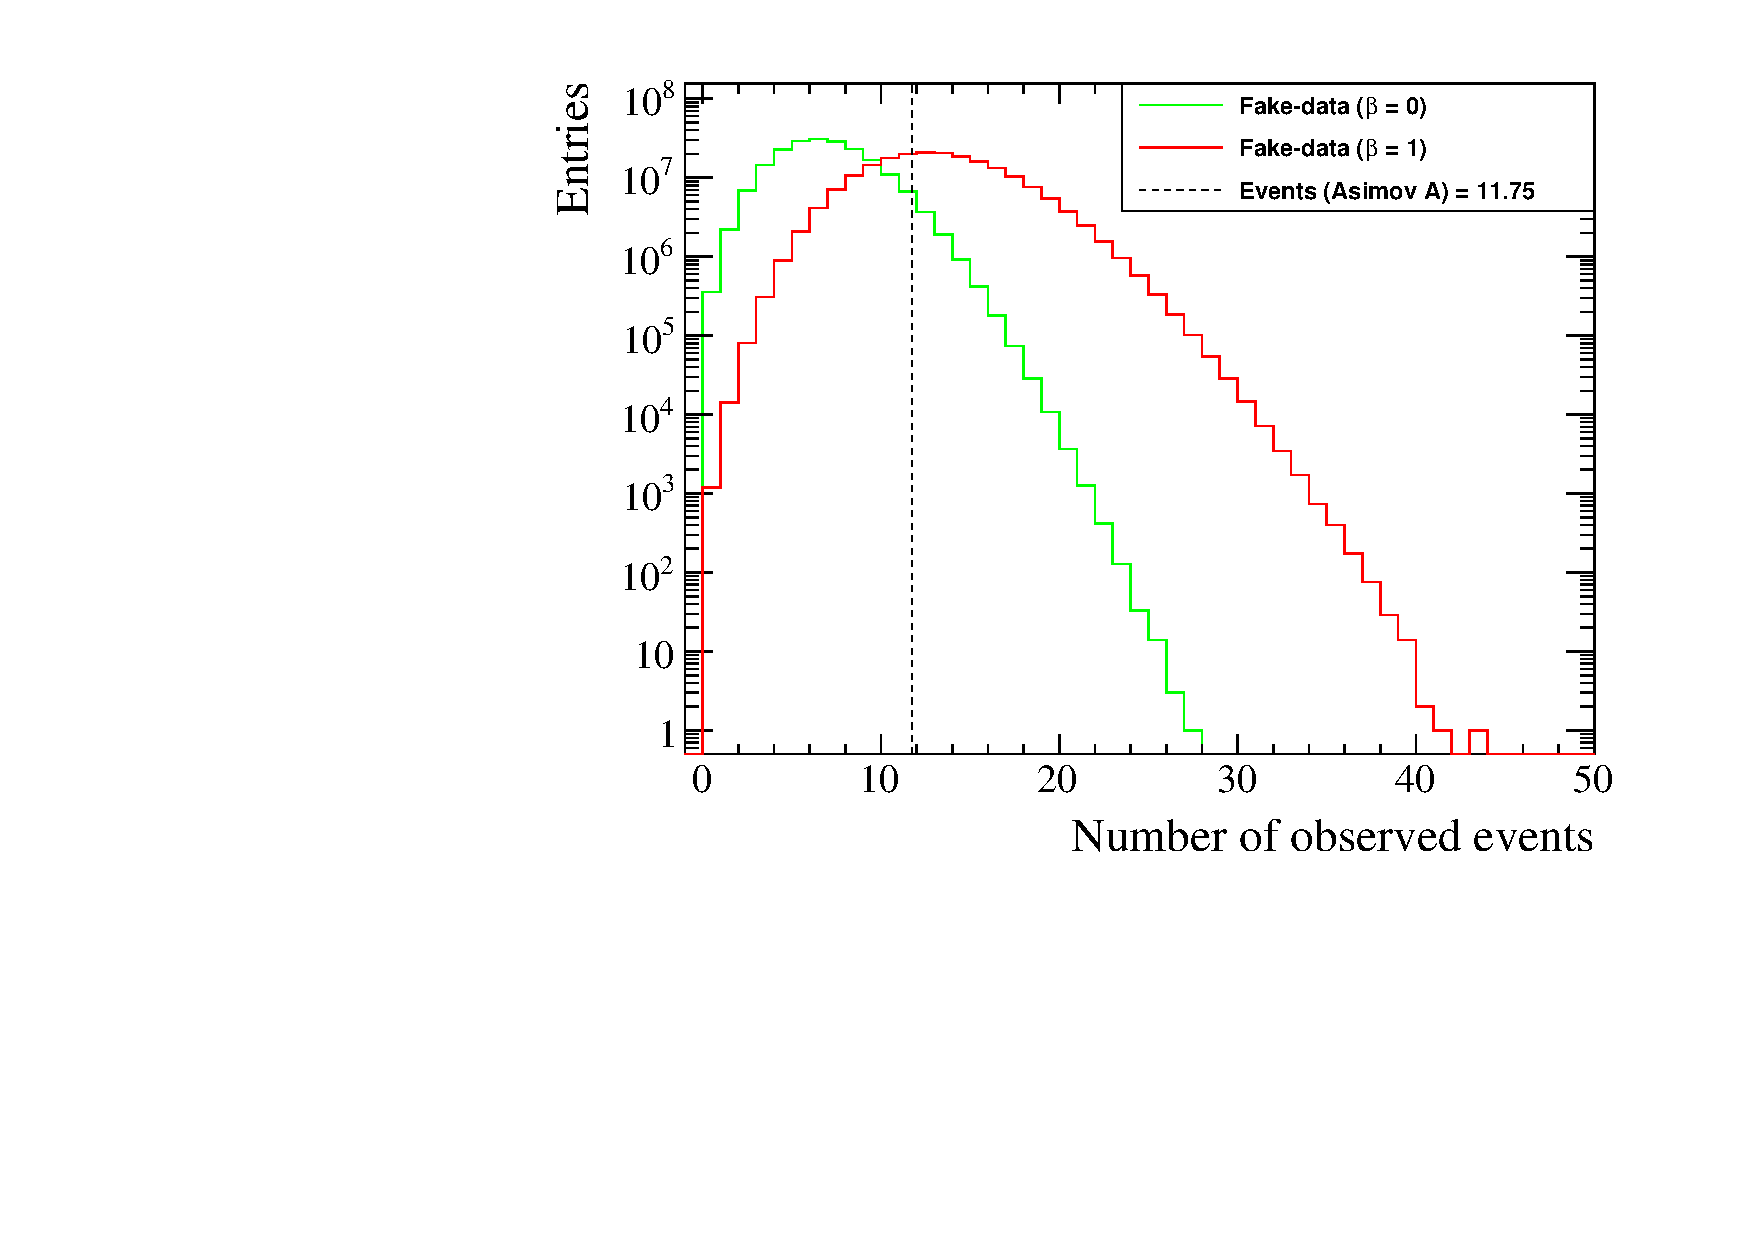
\includegraphics[scale=0.65]{sensitivity/plots_weighted_2018-04-06/rate-only_20ktoys/nuebarapp_graphs_nmargtoys=200k_nexp=20k_rate-only_posterior-predictive_VALORonly_nevents}
	\caption{The distribution of the total number of events in the antineutrino mode single-ring e-like sample from each of the \NToysFakeDataRateOnly\ toy experiments for both the $\beta = 0$ and $\beta = 1$ hypotheses. The distributions were produced using the method outlined in section \ref{sec:method_rate-only} using the Asimov A spectra to calculate the 4-sample likelihood. The dashed line corresponds to the total number of events given by the Asimov A data set.}
	\label{fig:sensitivity_rate-only}
\end{figure}

\begin{figure}
	\centering
	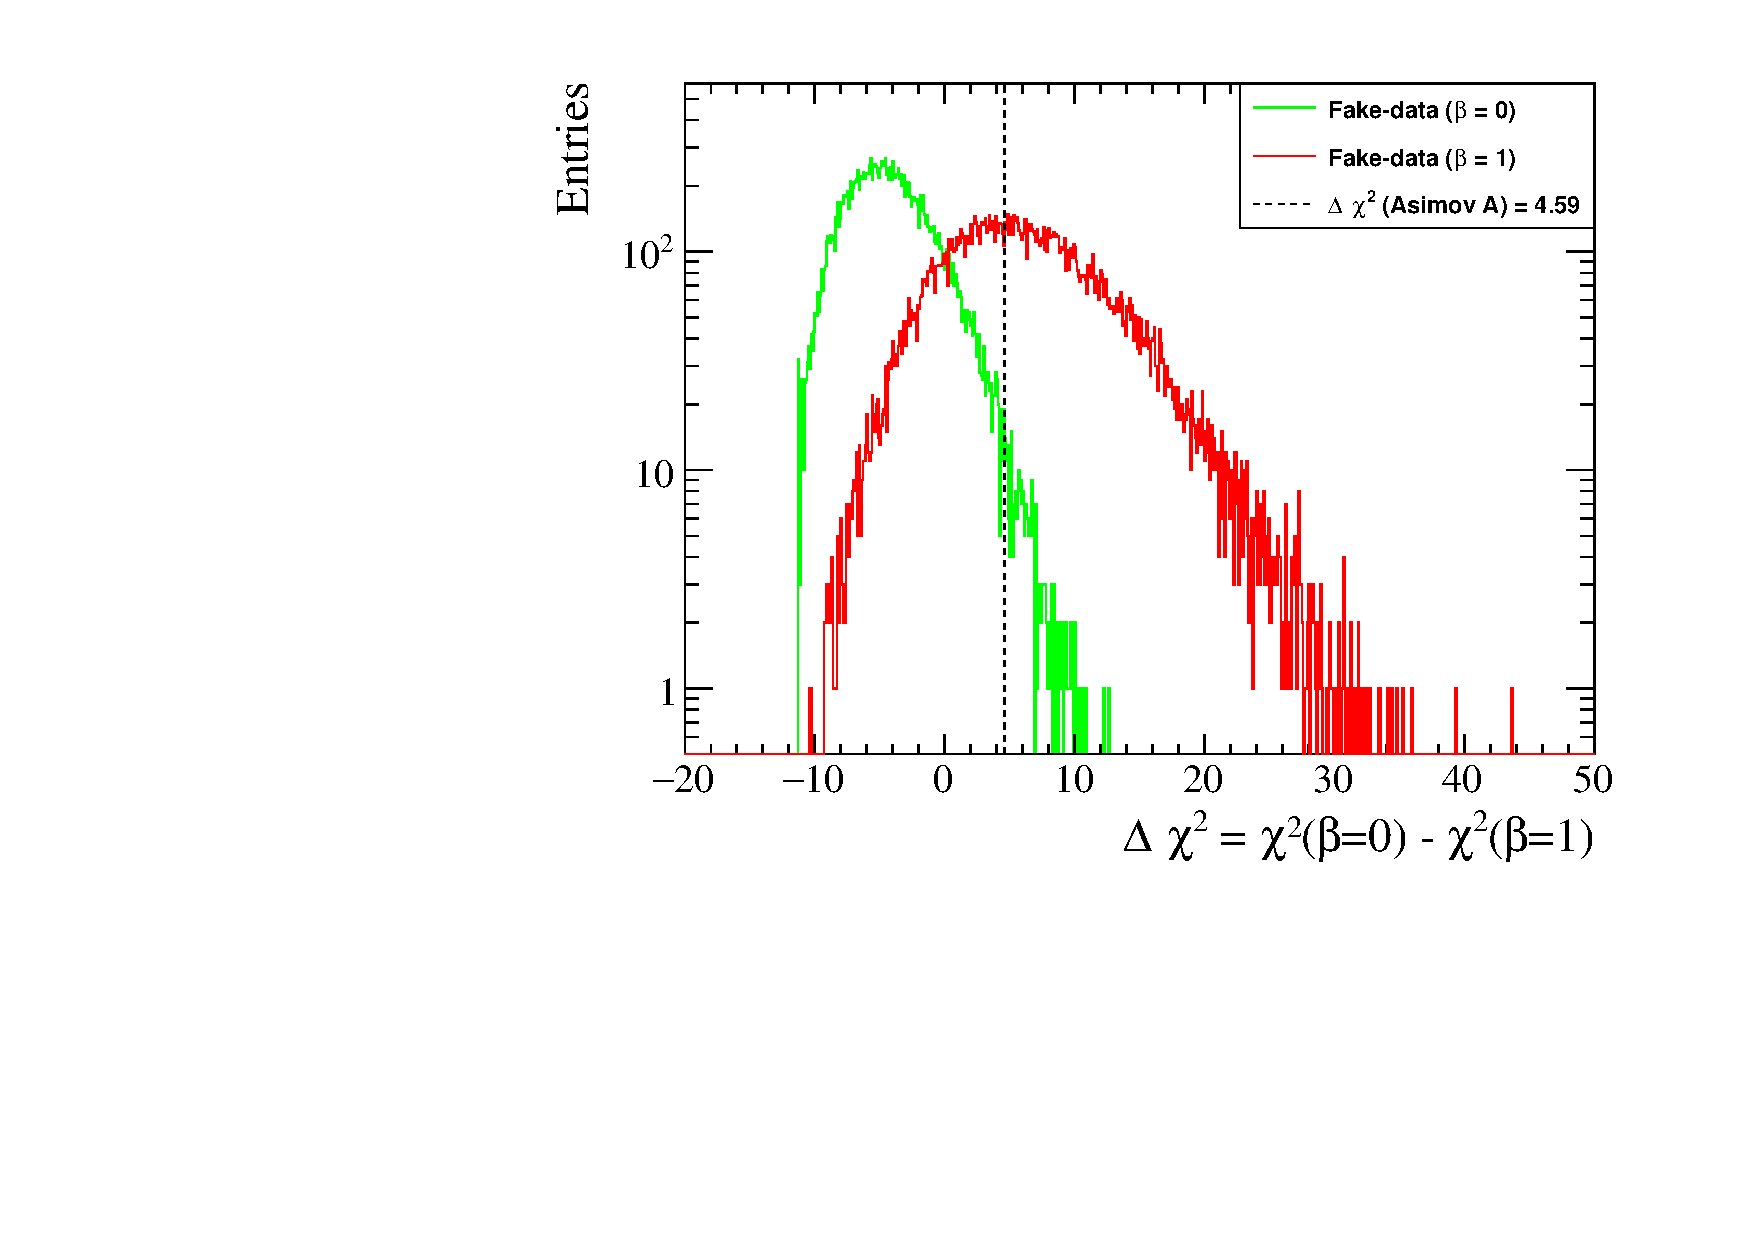
\includegraphics[scale=0.65]{sensitivity/plots_weighted_2018-04-06/rate+shape_20ktoys/nuebarapp_graphs_nmargtoys=200k_nexp=20k_rate+shape_posterior-predictive_VALORonly_Deltachisq_logscale}
	\caption{The distribution of $\Delta \chi^2$ values from each of the \NToysFakeDataRatePlusShape\ toy experiments for both the $\beta = 0$ and $\beta = 1$ hypotheses. The distributions were produced using the method outlined in section \ref{sec:method_rate+shape} using the Asimov A spectra to calculate the 4-sample likelihood. The dashed line corresponds to the $\Delta \chi^2$ value given by the Asimov A data set.}
	\label{fig:sensitivity_rate+shape}
\end{figure}


\section {Results of the $\nueb$ Appearance Analysis}
\label{sec:results}
The rate-only and rate+shape p-values for $\nueb$ appearance are performed on the combined \RunPeriod statistics following the same procedure as in Sec \ref{sec:method}. 1-sided p-values are computed on the right tail of the test statistic expected distribution to exclude $\beta = 0$ and the left tail to exclude $\beta = 1$. Fig \ref{fig:asimova_spectra_all} shows the data in the 5 Super-K event samples overlaid with the expected event rates for Asimov data set A. A summary of the observed number of events in Super-K, $\Delta \chi^2$ and p-values is given in Tab \ref{tab:data_comparison_R19c_R17}.



In Figs \ref{fig:data_rate-only} and \ref{fig:data_rate+shape} the distributions of the test statistic, for rate-only and rate+shape analyses, are shown and compared with the data. Tab \ref{tab:data_comparison_R19c_R17} contains a summary of the results. The rate-only analysis disfavours each hypothesis almost equally, whilst the rate+shape analysis disfavours the $\beta = 1$ hypothesis more than the $\beta = 0$ hypothesis. The Jeffreys scale indicates that the Bayes factor of \BayesFactorData\ corresponds to a poor preference for the $\beta = 0$ hypothesis over $\beta = 1$. %In comparison to the Run 1-7 analyses, the preference for $\beta = 0$ remains but has grown weaker. 
In comparison to the Run 1-7 analysis, the rate-only $\beta = 0$ p-value has decreased by a factor of 0.51. This is due to the number of observed events per POT increasing by a factor of 1.5, increasing the amount that the $\beta = 0$ hypothesis is disfavoured. The rate+shape $\beta = 0$ p-value has decreased by a factor of 0.57. In addition to the number of observed events per POT increasing by a factor of 1.5, this can be explained by an increase in the number of events (compared to the Run 1-7 analysis \cite{OurRun16AntiNueBarAppearanceAnalysis3Flavour}) in regions of the spectra in Fig \ref{fig:nuebar_tot_spectra} where a larger number of events are expected.

The P-theta rate-only p-values for the \RunPeriod data set are \PthetaPvalDataRateOnlyBetaZero\ and \PthetaPvalDataRateOnlyBetaOne\ for $\beta = 0$ and $\beta = 1$, respectively and the rate+shape p-values (using $E_{reco}-\theta$) are \PthetaPvalDataRateShapeErecThetaBetaZero\ and \PthetaPvalDataRateShapeErecThetaBetaOne\ for $\beta = 0$ and $\beta = 1$, respectively \cite{PthetaR19cNuebarAppearance}. The p-values produced by the VALOR and P-theta groups are considered to be within acceptable agreement. {\color{red} During the Run1-9c analysis,} the reason for the remaining differences between the VALOR and P-theta p-values {\color{red}were} thought to be due to differences in the toy generation methods. {\color{red} A comparison of the toy generation methods is shown in appendix \ref{app:sampling_vs_reweighting} using full Run 1-9 statistics.}

By breaking the electron-like antineutrino mode spectra from Fig \ref{fig:asimova_spectra_all} into its components, as shown in Fig \ref{fig:asimova_spectra_components}, some explanation can be offered for the preference for the no $\nueb$ appearance hypothesis. The observed events do not appear to fit the Asimov A expected $\numub \rightarrow \nueb$ distribution well, instead they are more consistent with the $\numu \rightarrow \nue$ and intrinsic $\nue\ \&\ \nueb$ backgrounds. As the shape of the spectra discredits the $\beta = 1$ hypothesis (which is information that the rate-only analysis does not have access to), the $\beta = 1$ p-value for the rate+shape analysis is substantially smaller than that of the rate-only analysis.

\FloatBarrier

\begin{figure*}[htb]
	\center
	\begin{subfigure}[b]{0.49\textwidth}
		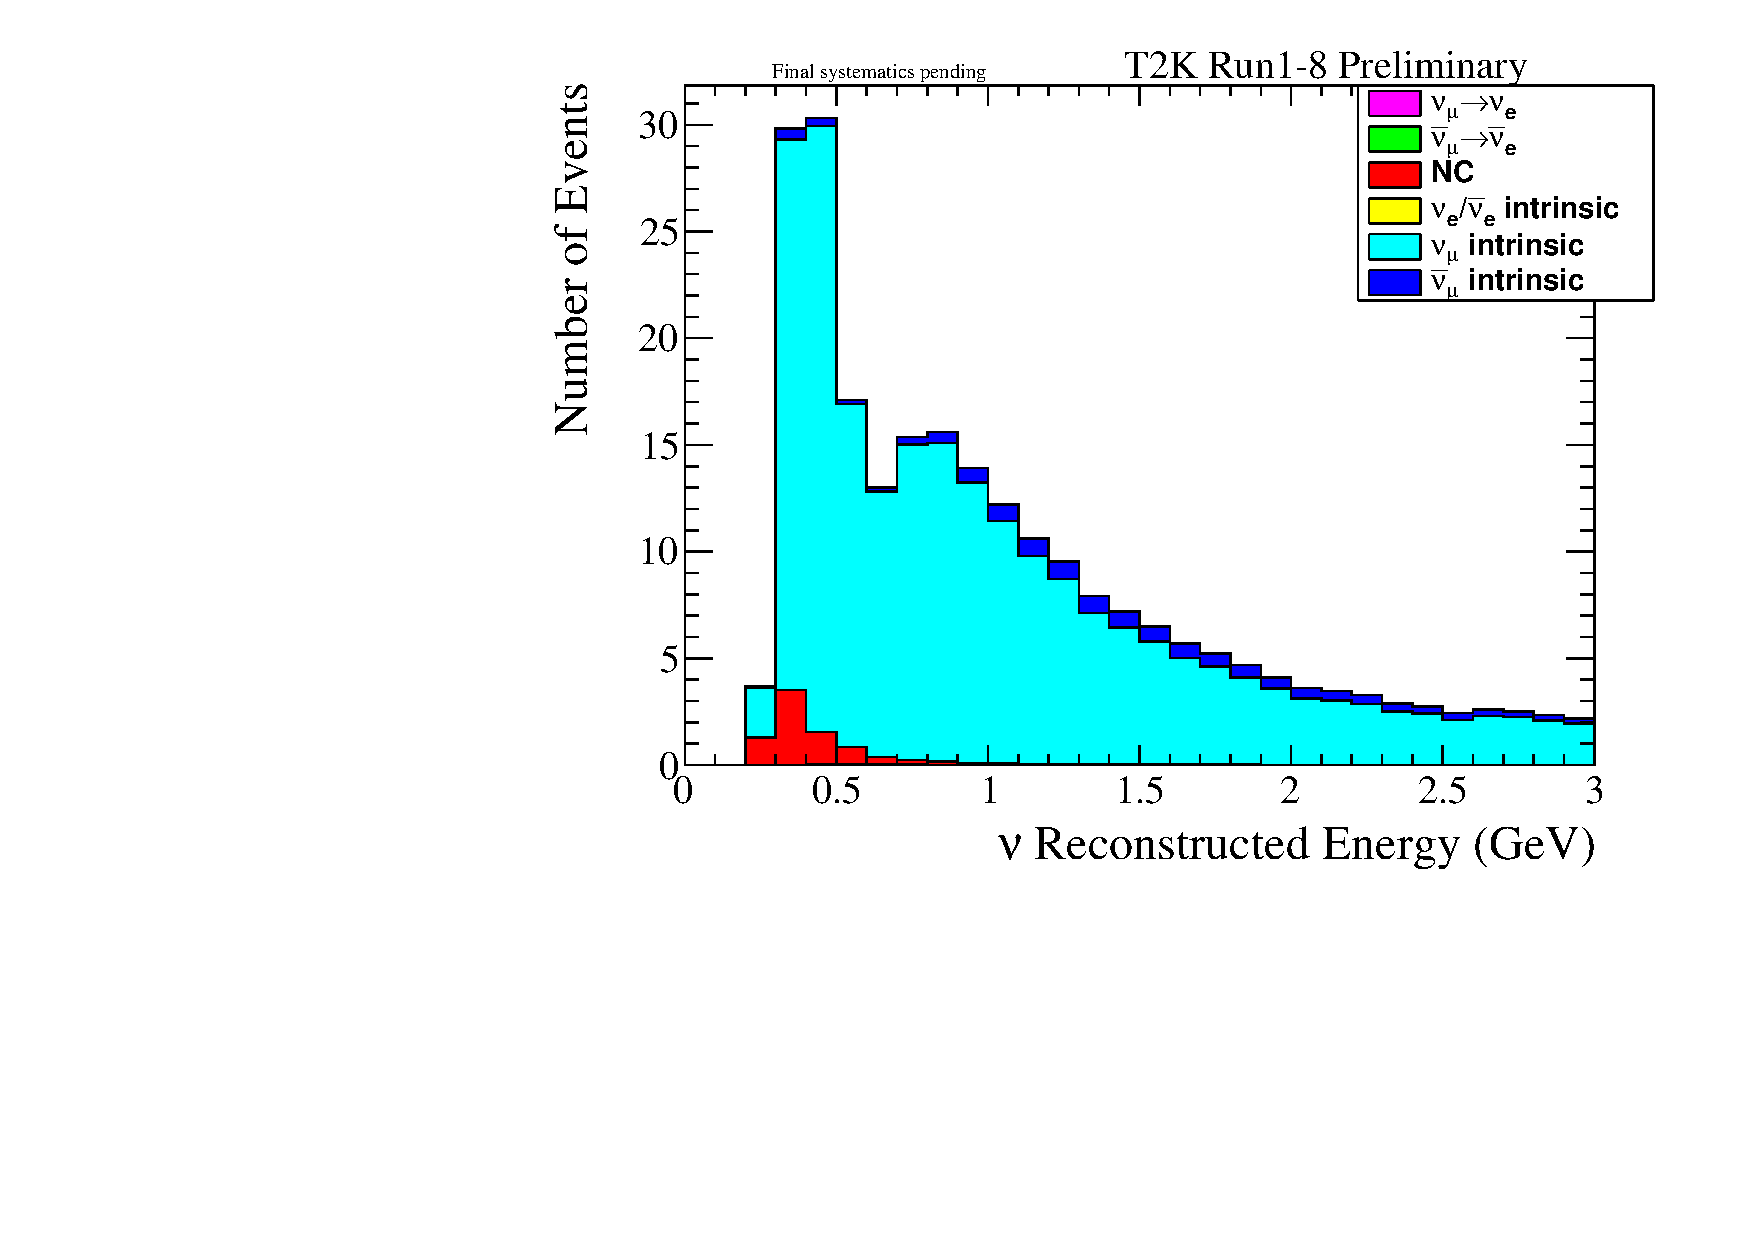
\includegraphics[width=0.9\textwidth]{spectra/spectrum_osc_asimova_1Rmu}
		\caption{Muon-like, neutrino mode}
	\end{subfigure}
	\begin{subfigure}[b]{0.49\textwidth}
		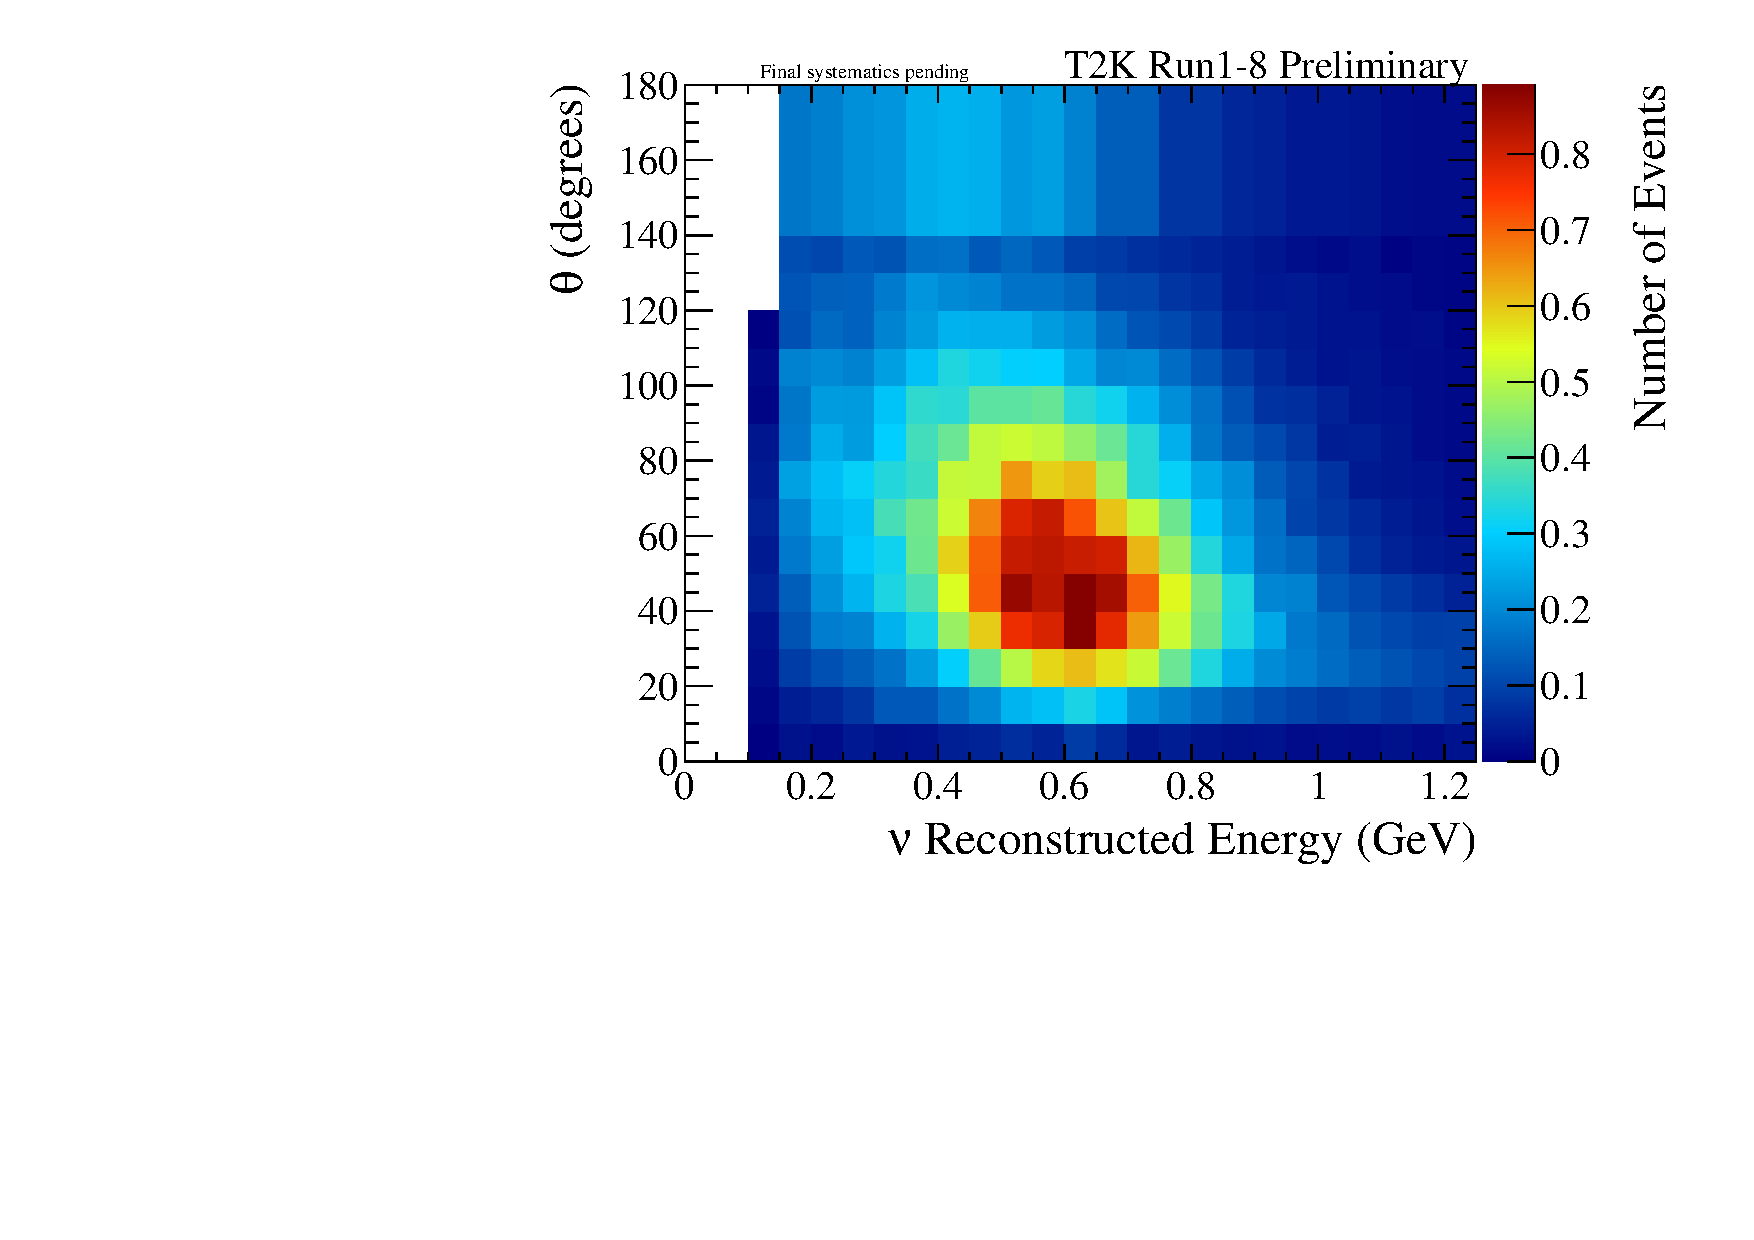
\includegraphics[width=0.9\textwidth]{spectra/spectrum_osc_asimova_1Re}
		\caption{Electron-like, neutrino mode}
	\end{subfigure}
	\begin{subfigure}[b]{0.49\textwidth}
		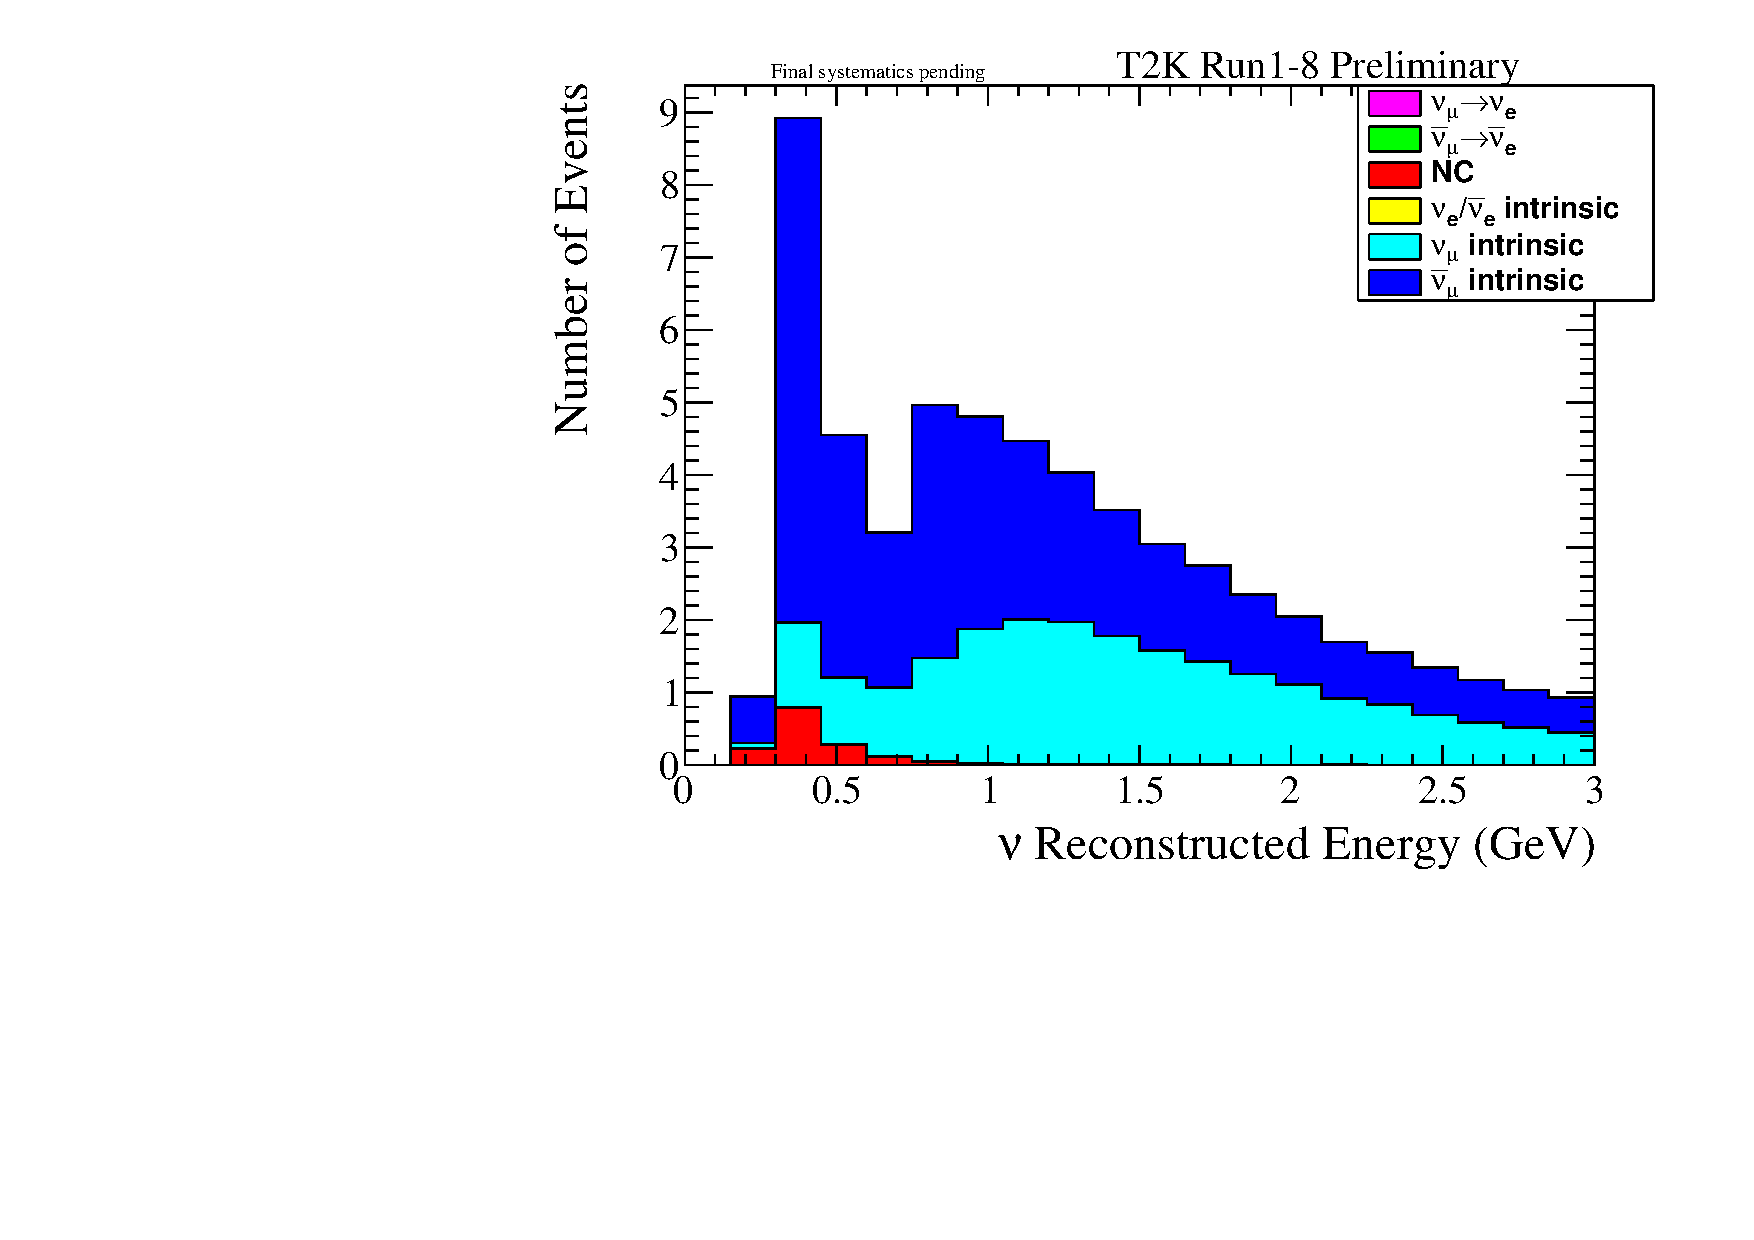
\includegraphics[width=0.9\textwidth]{spectra/spectrum_osc_asimova_RHC1Rmu}
		\caption{Muon-like, antineutrino mode}
	\end{subfigure}
	\begin{subfigure}[b]{0.49\textwidth}
		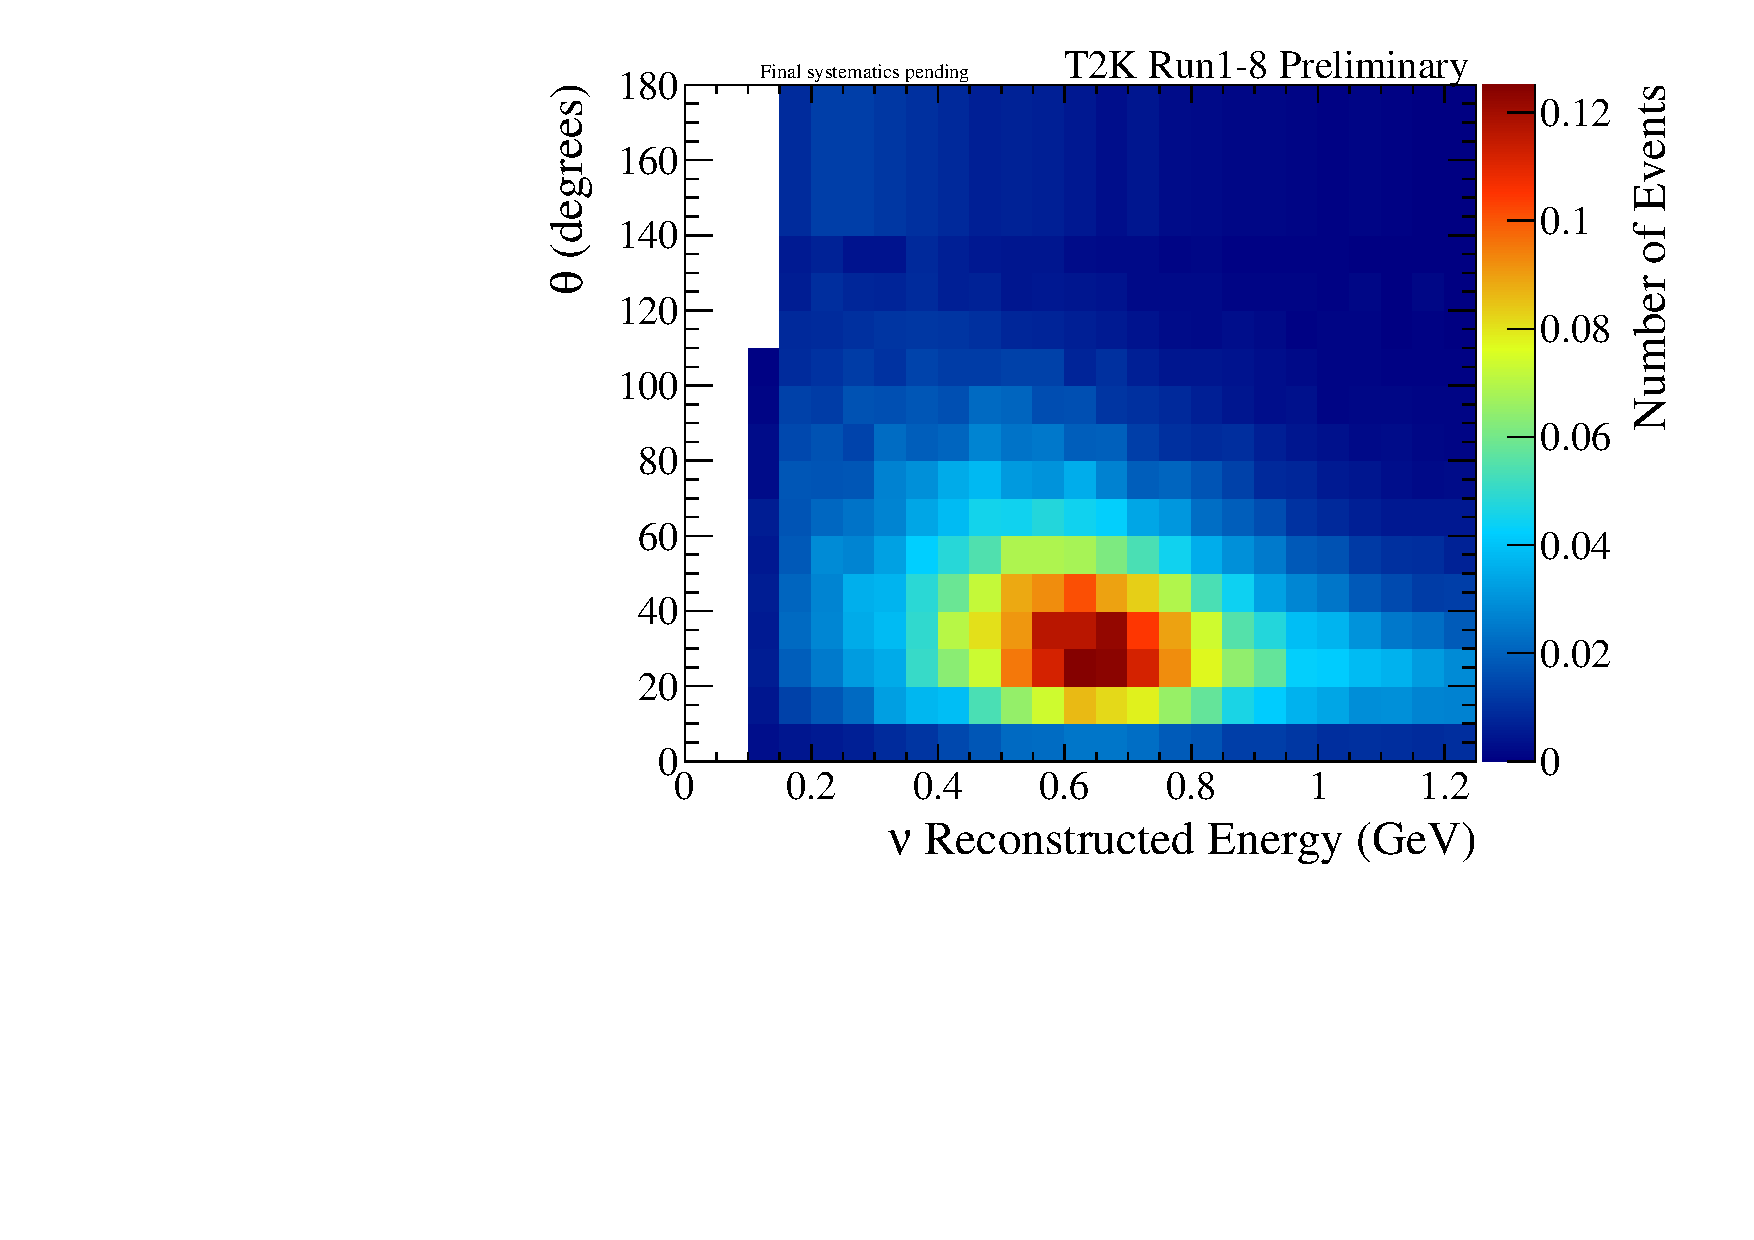
\includegraphics[width=0.9\textwidth]{spectra/spectrum_osc_asimova_RHC1Re}
		\caption{Electron-like antineutrino mode}
	\end{subfigure}
	\begin{subfigure}[b]{0.49\textwidth}
		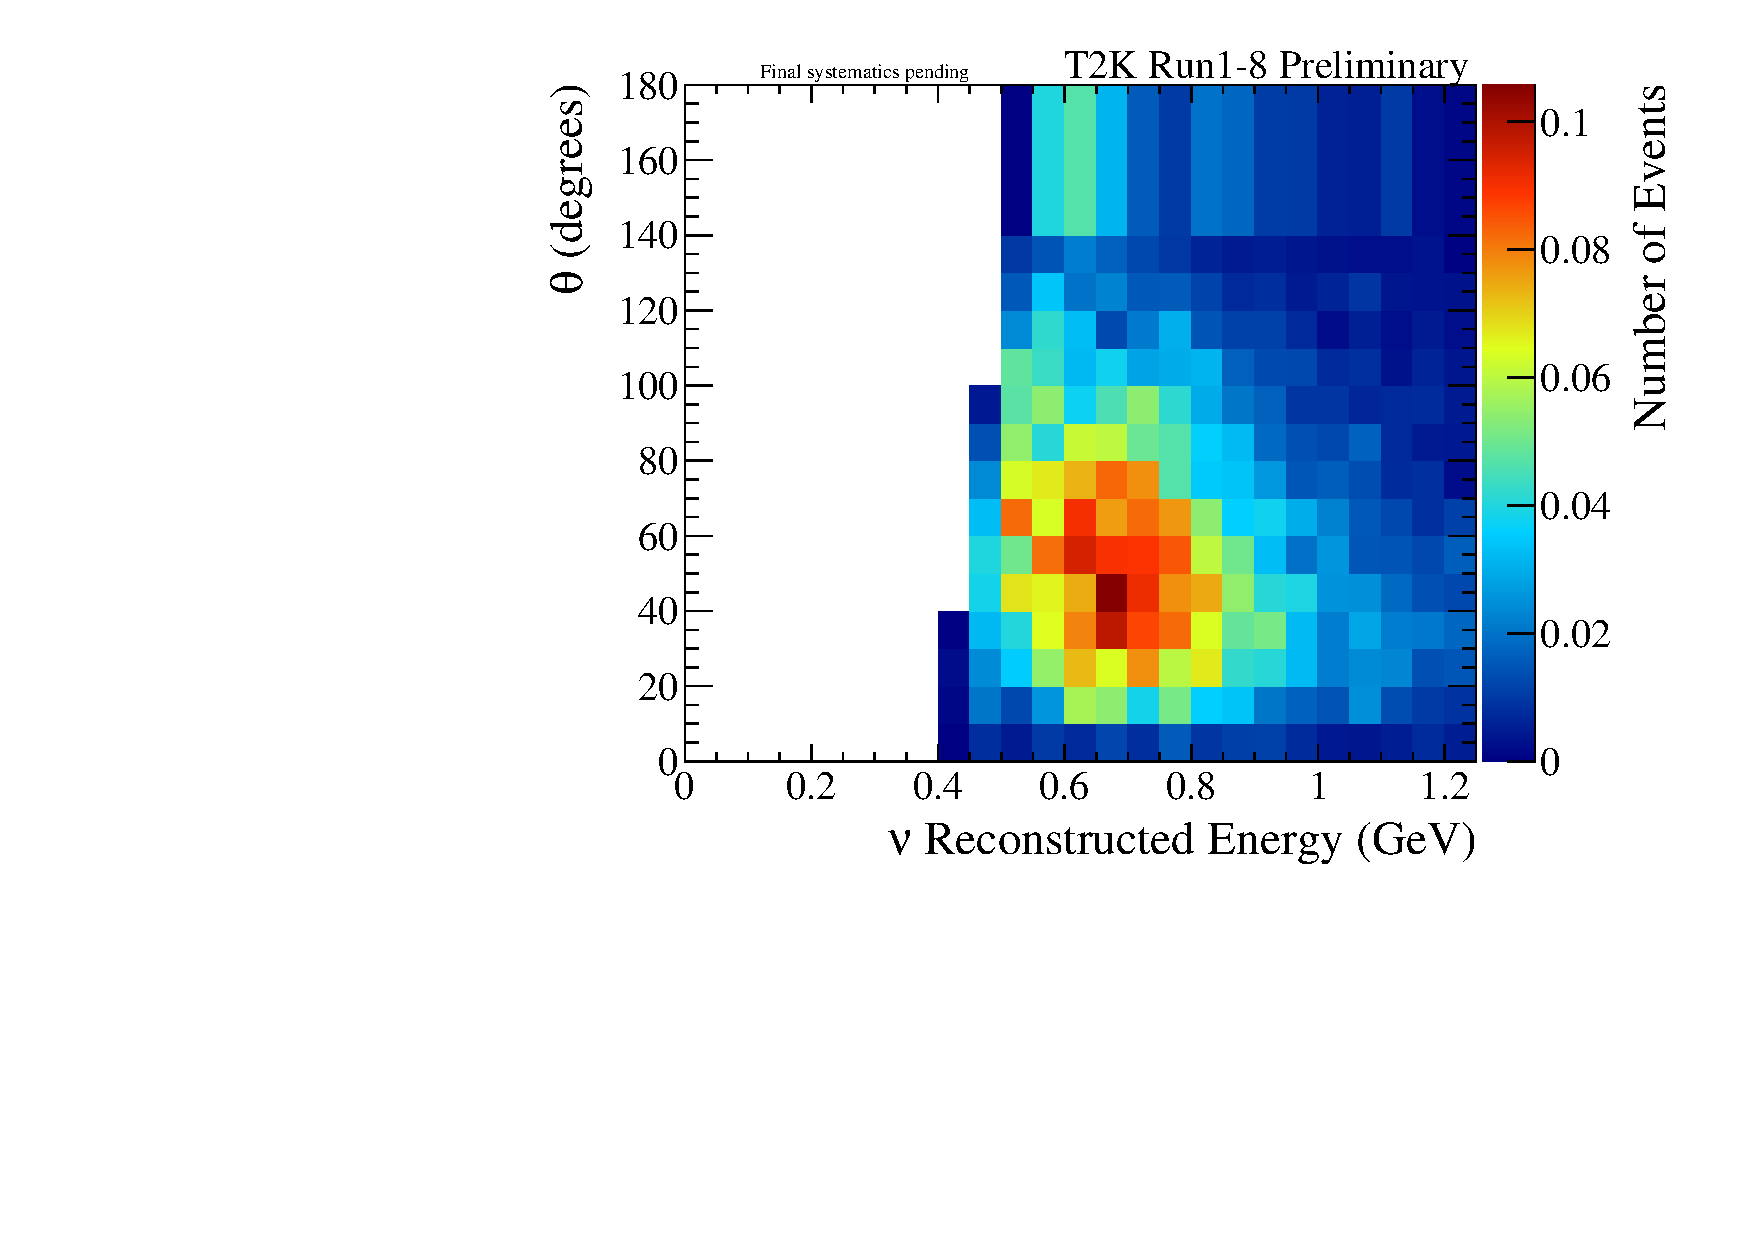
\includegraphics[width=0.9\textwidth]{spectra/spectrum_osc_asimova_MultiRe}
		\caption{\nueCConepi-like, neutrino mode}
	\end{subfigure}
	\caption {
		Predicted Asimov A spectra. $\mu$-like distributions are a function of the reconstructed neutrino energy, while the $e$-like, including \nueCConepi, distributions are functions of both the reconstructed neutrino energy and the reconstructed angle between the outgoing lepton and the neutrino direction. The distributions correspond to the statistics collected in the full \RunPeriod data set. The spectra are generated with the systematic parameters described in \cref{sec:systematics} and the oscillation parameters corresponding to the Asimov data set A shown in \cref{tab:asimov_definition1}.
	}
	\label{fig:asimova_spectra_all}
\end{figure*}
\clearpage

\begin{figure}
	\centering
	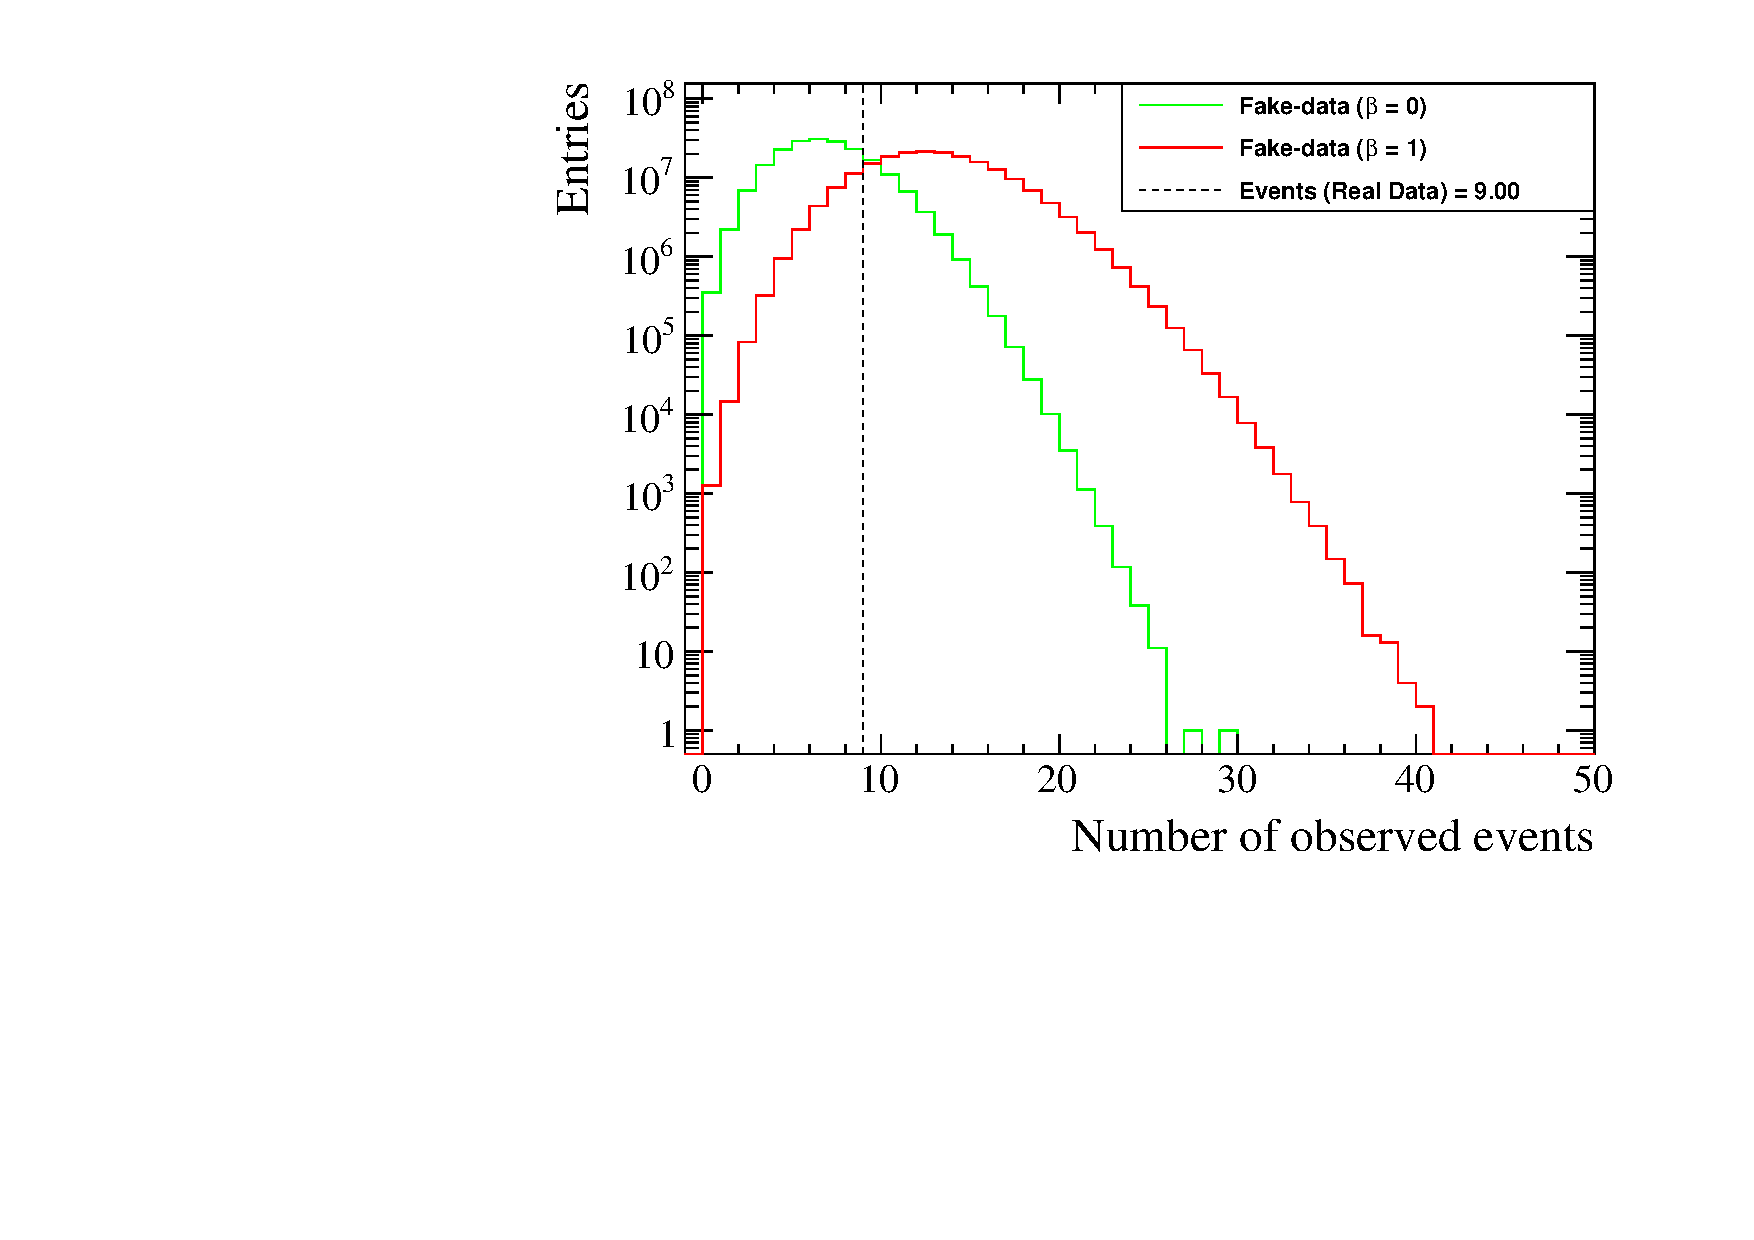
\includegraphics[scale=0.65]{data/nuebarapp_graphs_nmargtoys=200k_nexp=20k_rate-only_posterior-predictive_VALORonly_nevents}
	\caption{The distribution of the total number of events in the antineutrino mode single-ring e-like sample from each of the \NToysFakeDataRateOnly\ toy experiments for both the $\beta = 0$ and $\beta = 1$ hypotheses. The distributions were produced using the method outlined in section \ref{sec:method_rate-only} using the \RunPeriod data spectra to calculate the 4-sample likelihood. The dashed line corresponds to the total number of events given by the \RunPeriod data set.
	}
	\label{fig:data_rate-only}
\end{figure}

\begin{figure}
	\centering
	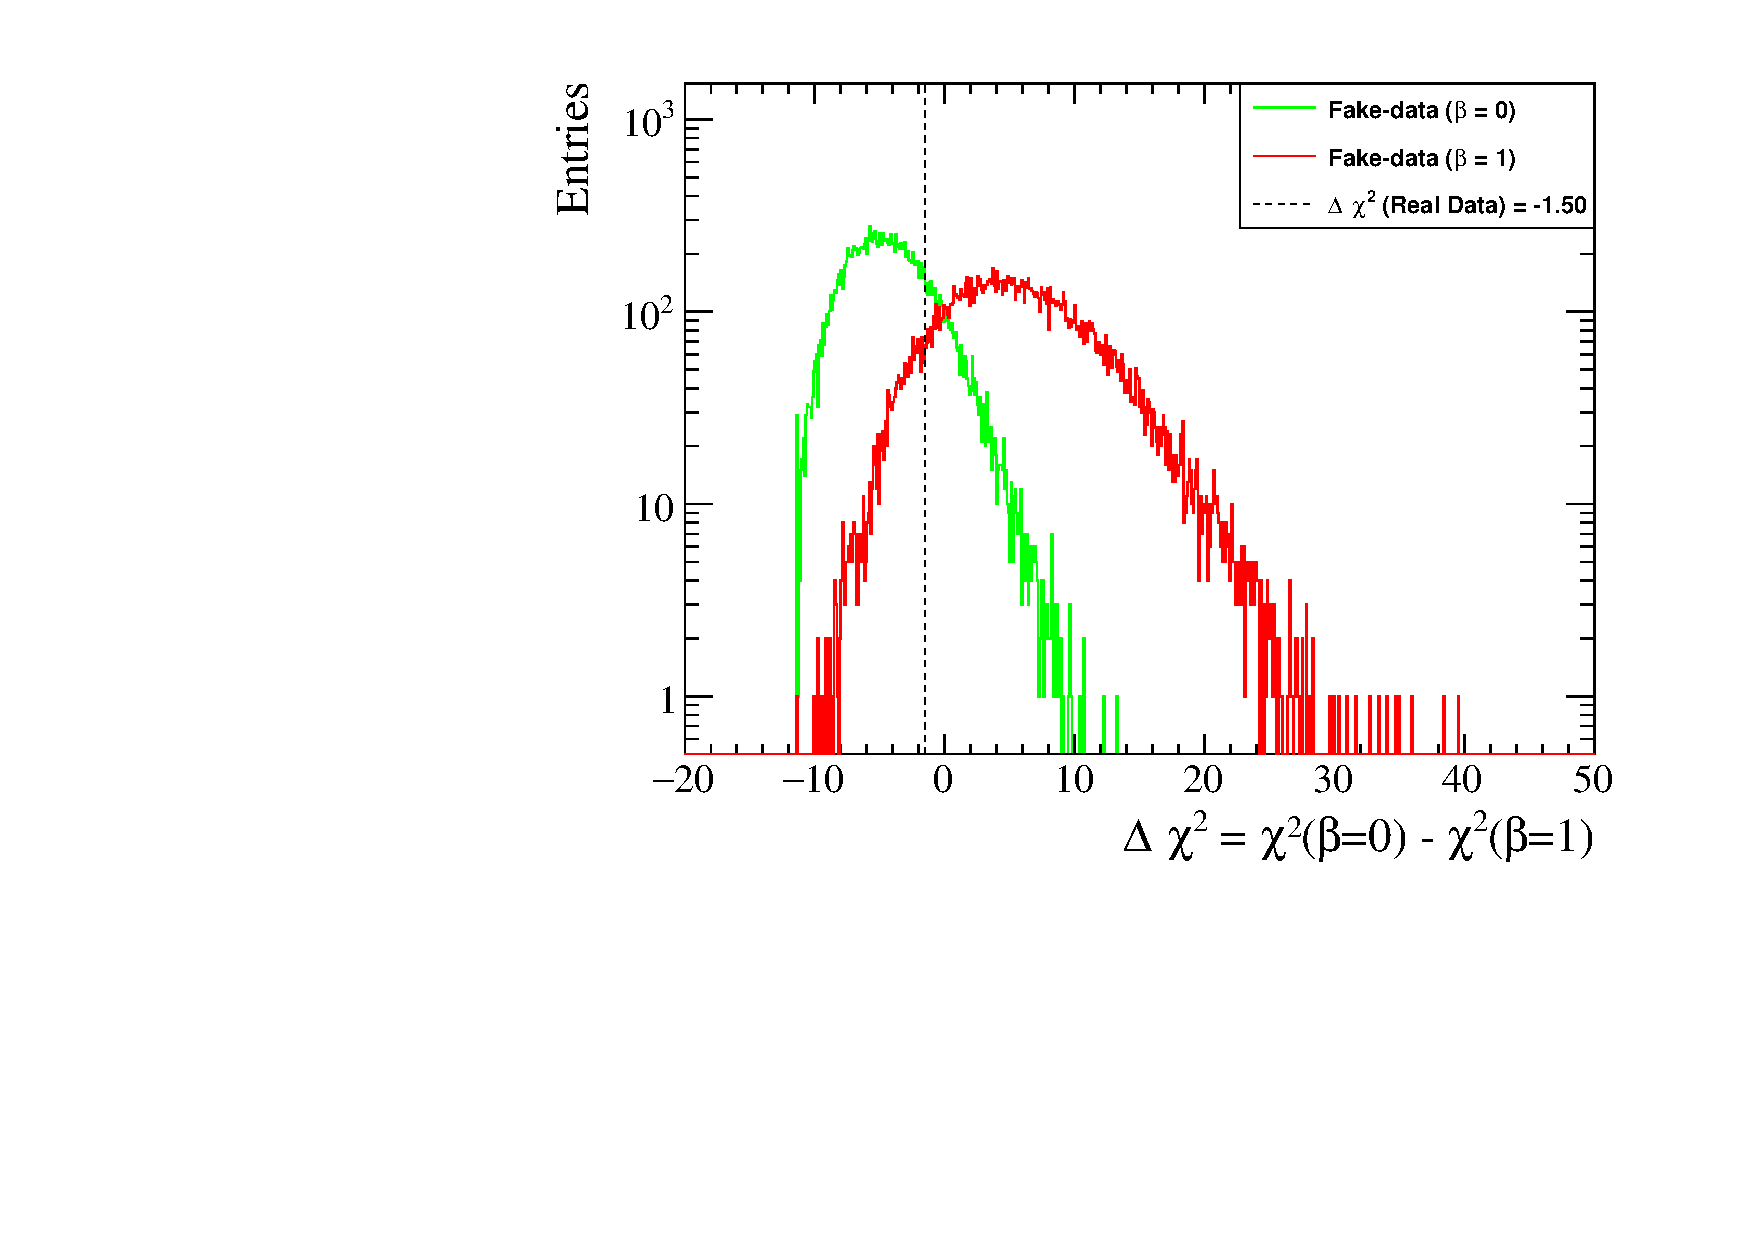
\includegraphics[scale=0.65]{data/nuebarapp_graphs_nmargtoys=200k_nexp=20k_rate+shape_posterior-predictive_VALORonly_Deltachisq_logscale}
	\caption{The distribution of $\Delta \chi^2$ values from each of the \NToysFakeDataRatePlusShape\ toy experiments for both the $\beta = 0$ and $\beta = 1$ hypotheses. The distributions were produced using the method outlined in section \ref{sec:method_rate+shape} using the \RunPeriod data spectra to calculate the 4-sample likelihood. The dashed line corresponds to the $\Delta \chi^2$ value given by the \RunPeriod data set.
	}
	\label{fig:data_rate+shape}
\end{figure}

\FloatBarrier

\begin{table}
	\centering
	\begin{tabular}{|c|c|c|c|c|c|c|c|c|}
		\hline
		\multirow{2}{*}{Run} & \multirow{2}{*}{RHC POT}   & \multicolumn{3}{|c|}{Rate-only Analysis}  			    & \multicolumn{4}{|c|}{Rate+shape Analysis} \\
		\cline{3-9}     				
		     		&                            & $N_{obs}$  					& $\beta = 0$ p-value       & $\beta = 1$ p-value      & $\Delta \chi^2_{\textrm{obs}}$  & $\beta = 0$ p-value        & $\beta = 1$ p-value       & \textbf{$B_{01}$} \\
		\hline
		1-9c  & \TotalPotNuBarRunOneNineC  & \NskObservedNueBarRunOneNineC & \pvalRateOnlyBetaZeroData & \pvalRateOnlyBetaOneData & \DeltachisqData  & \pvalRateShapeBetaZeroData & \pvalRateShapeBetaOneData & \BayesFactorData \\
		\hline
		1-7     & \TotalPotNuBarRunOneSevenC & 4			  					& 0.410						& 0.2155				   & -1.930			  & 0.3742					   & 0.099					  & 2.62 \\
		\hline
	\end{tabular}
	\caption{Summary of observed number of events, $\Delta \chi^2$, rate-only and rate+shape p-values and Bayes factor from the combined \RunPeriod data set compared to the Run 1-7 data set used for the previous iteration of this analysis, in 2016 \cite{OurRun16AntiNueBarAppearanceAnalysis3Flavour}.}
	\label{tab:data_comparison_R19c_R17}
\end{table}

%TODO: POT column as well?


\begin{figure*}[htb]
	\center
	\begin{subfigure}[b]{0.49\textwidth}
		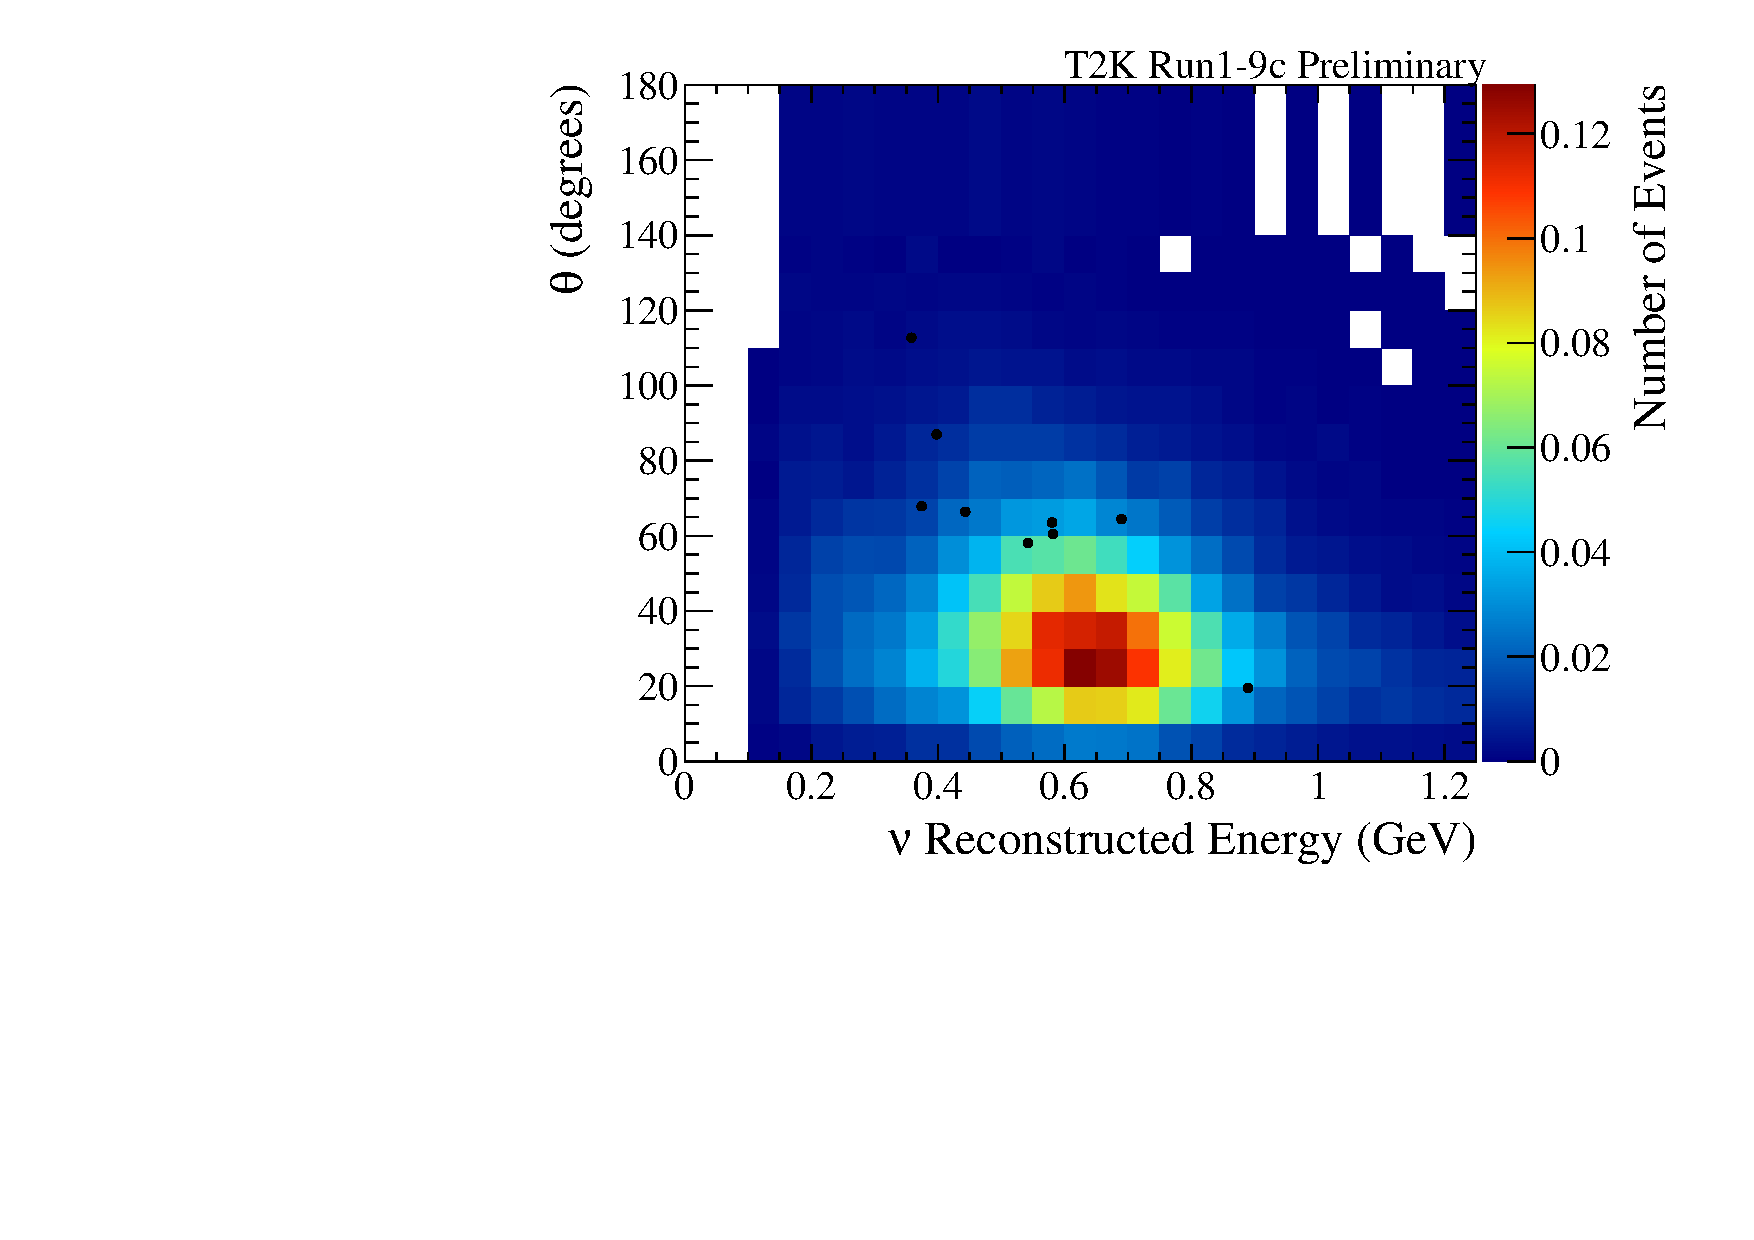
\includegraphics[width=0.9\textwidth]{spectra/components/spectrum_AsmovA_RHC1Re_NumuBarToNueBar}
		\caption{$\numub \rightarrow \nueb$}
	\end{subfigure}
	\begin{subfigure}[b]{0.49\textwidth}
		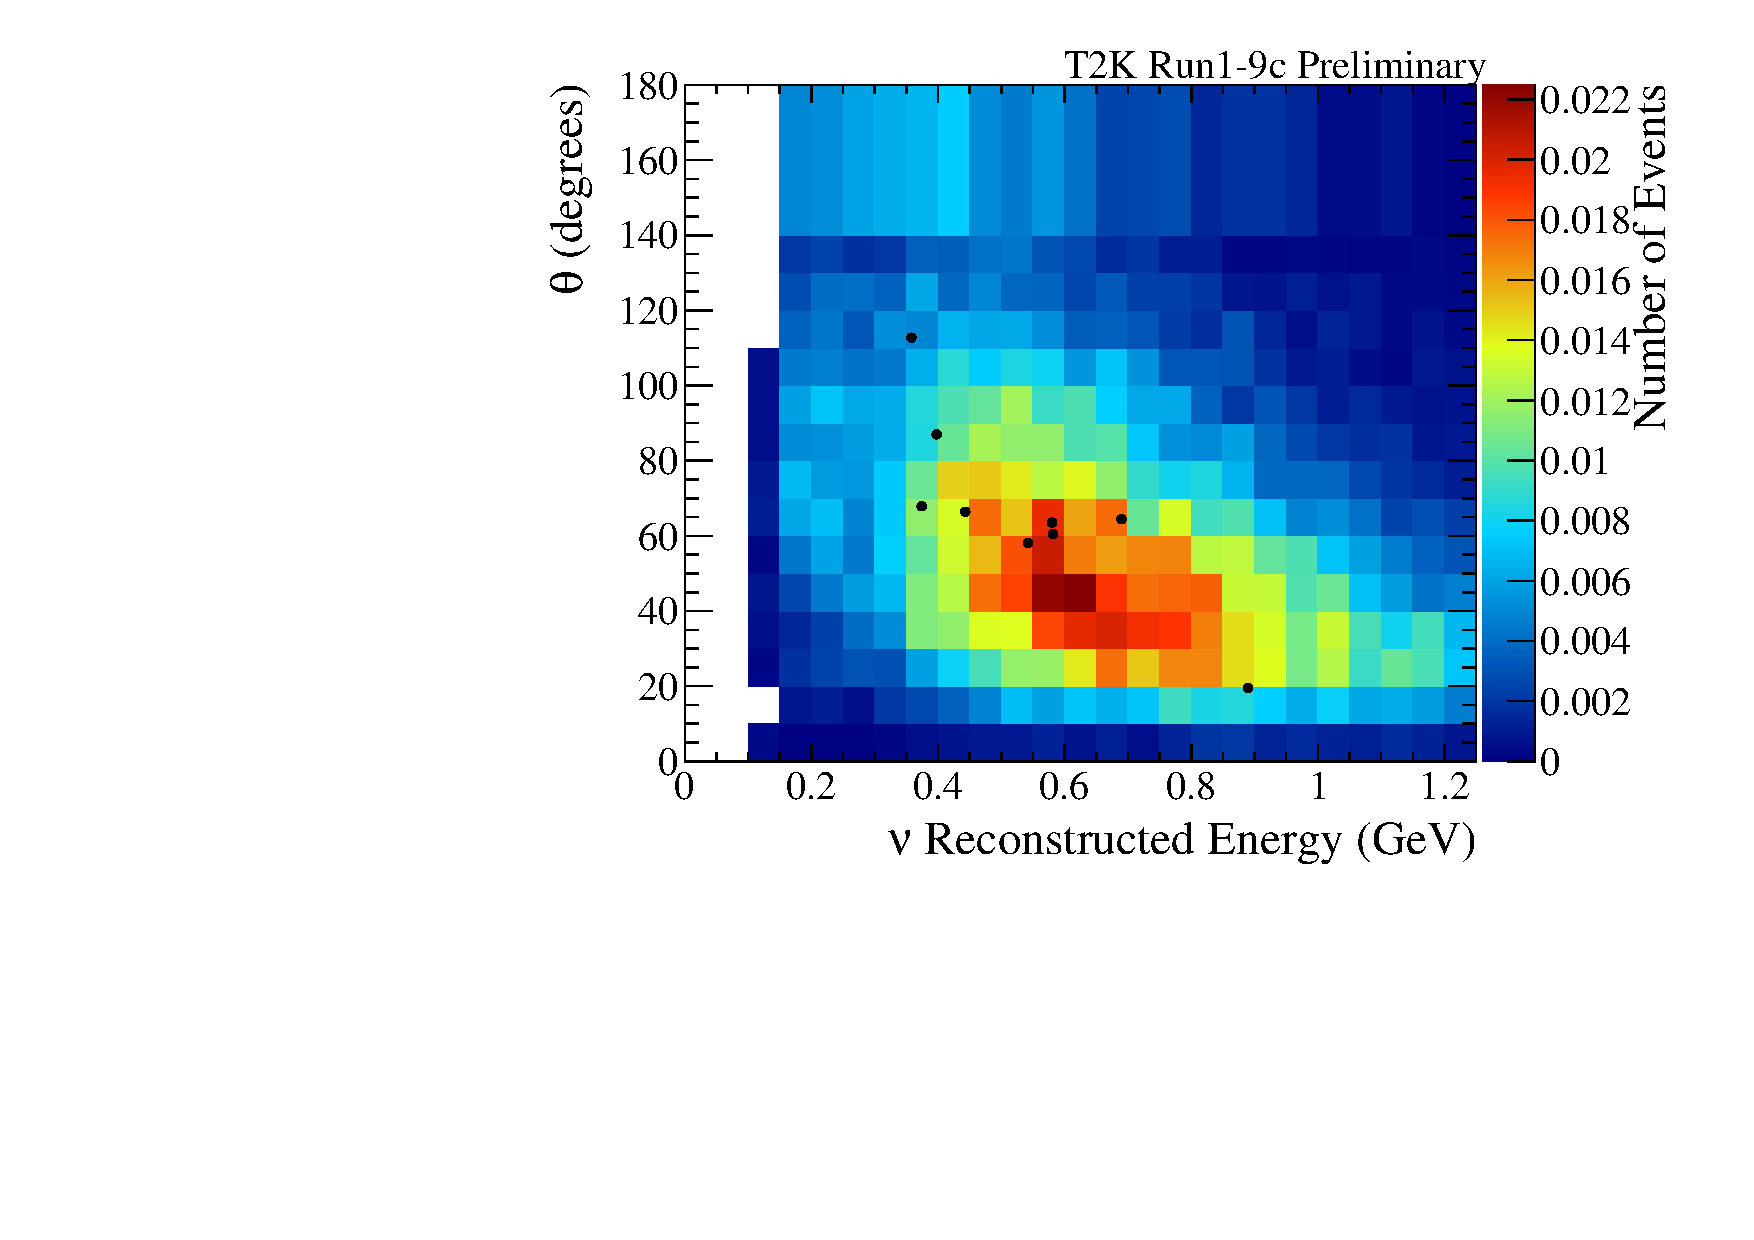
\includegraphics[width=0.9\textwidth]{spectra/components/spectrum_AsmovA_RHC1Re_NumuToNue}
		\caption{$\numu \rightarrow \nue$}
	\end{subfigure}
	\begin{subfigure}[b]{0.49\textwidth}
		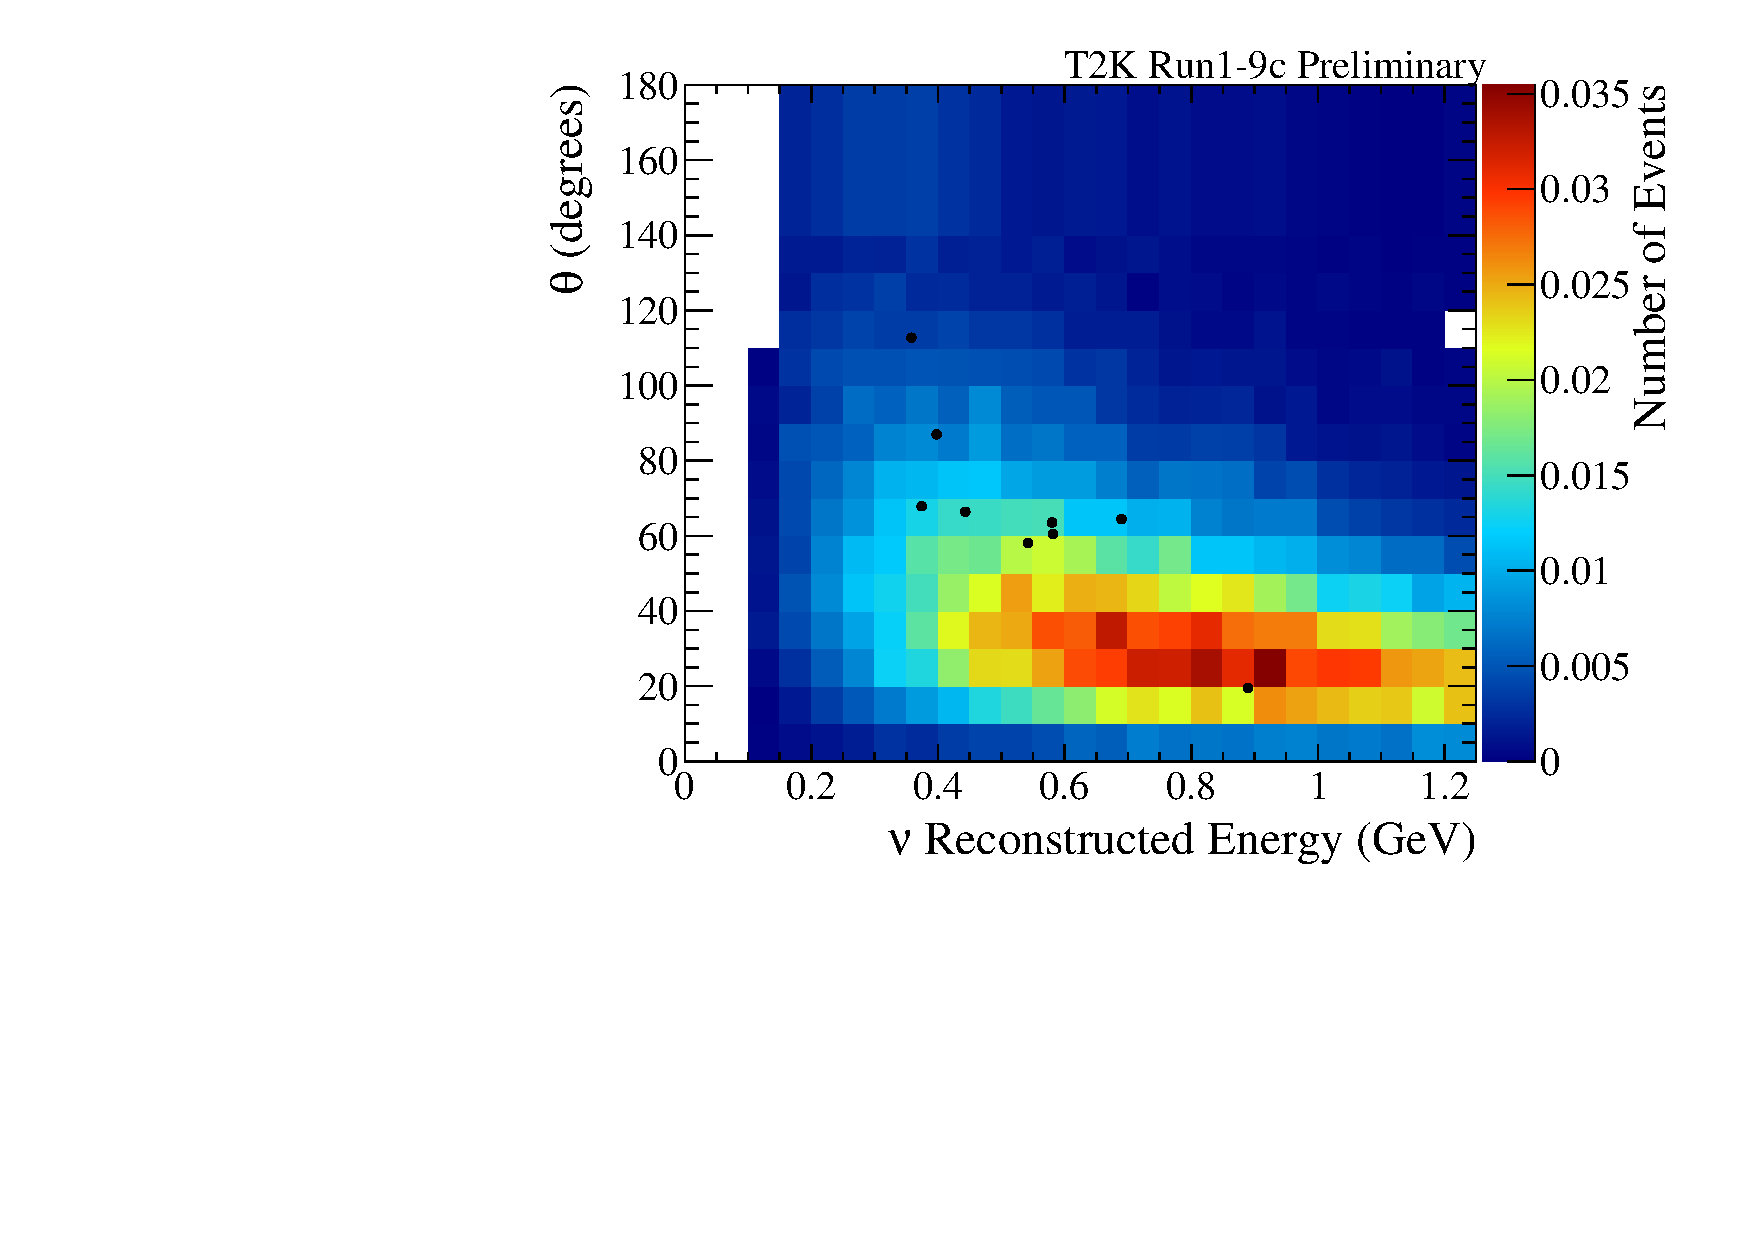
\includegraphics[width=0.9\textwidth]{spectra/components/spectrum_AsmovA_RHC1Re_NueBeam}
		\caption{Intrinsic $\nue$ + Intrinsic $\nueb$}
	\end{subfigure}
	\caption {
		Predicted Asimov A Electron-like antineutrino mode spectra broken down by component. The distributions correspond to the statistics collected in the full \RunPeriod data set. The spectra are generated with the oscillation parameters corresponding to the Asimov data set A shown in \cref{tab:osc_params_joint_asimovA}.
	}
	\label{fig:asimova_spectra_components}
\end{figure*}
\clearpage

\FloatBarrier
\section {Summary}
\label{sec:summary}

In this technical note, we have presented the results of the $\nueb$ appearance analysis using the 3-flavour $\nu$/$\bar{\nu}$ joint analysis framework performed by the VALOR group, on the combined \RunPeriod data set, for an exposure of \TotalPotNuRunOneNineC\ POT in neutrino mode and \TotalPotNuBarRunOneNineC\ POT in antineutrino mode. The goal of the analysis is to search for $\nueb$ appearance in a $\numub$ beam.

This analysis predicts $\NskOscExpectationNumuRunOneNineC \pm \NskOscExpectationNumuErrorRunOneNineC$ (syst) for neutrino $\mu$-like, $\NskOscExpectationNumuBarRunOneNineC \pm \NskOscExpectationNumuBarErrorRunOneNineC$ (syst) for antineutrino $\mu$-like, $\NskOscExpectationNueRunOneNineC \pm \NskOscExpectationNueErrorRunOneNineC$ (syst) for neutrino e-like, $\NskOscExpectationNueBarRunOneNineC \pm \NskOscExpectationNueBarErrorRunOneNineC$ (syst) for antineutrino e-like and $\NskOscExpectationNueCConepiRunOneNineC \pm \NskOscExpectationNueCConepiErrorRunOneNineC$ (syst) for neutrino $\nu_{e}\textrm{CC}1\pi^{+}$-like events in Super K and observes respectively \NskObservedNumuRunOneNineC\ for neutrino $\mu$-like, \NskObservedNumuBarRunOneNineC\ for antineutrino $\mu$-like, \NskObservedNueRunOneNineC\ for neutrino e-like, \NskObservedNueBarRunOneNineC\ for antineutrino e-like and \NskObservedNueCConepiRunOneNineC\ for neutrino $\nu_{e}\textrm{CC}1\pi^{+}$-like events.

Both a rate only and a rate+shape analysis are performed. In both analyses, fits were performed in the joint fit framework, including all samples as data to constraint either background and the hypotheses tested. The number of observed events in the antineutrino mode e-like spectrum is \NskObservedNueBarRunOneNineC\ and the measured rate+shape test statistic, $\Delta \chi^2 = \chi^2\left( \beta = 0 \right) - \chi^2\left( \beta = 1 \right)$ was found to be \DeltachisqData. The significance of the result is shown as a p-value. Taking no $\nueb$ appearance as our null hypothesis we find a p-value of \pvalRateOnlyBetaZeroData\ for the rate-only analysis and a p-value of \pvalRateShapeBetaZeroData\ for the rate+shape analysis. Taking $\nueb$ appearance according to the best knowledge of the PMNS matrix as our null hypothesis we find a p-value of \pvalRateOnlyBetaOneData\ for the rate-only analysis and a p-value of \pvalRateShapeBetaOneData\ for the rate+shape analysis. The Bayes factor, given by the rate+shape analysis was found to be \BayesFactorData\, indicating a poor preference for no $\nueb$ appearance.
\clearpage

{\color{red} 

\section {Updated Analysis Using the Full T2K Run 1-9 Dataset} \label{sec:run1-9d_update}

A statistical update to the Run 1-9c results has been performed with the addition of the Run 9d dataset. The analysis procedure is identical to that of the Run 1-9c analysis, but there has been the following changes to the analysis inputs:

\begin{itemize}
	\item An increase of $\nub$ mode exposure of $\SI{46}{\%}$ from $\TotalPotNuBarRunOneNineC$ POT to $\TotalPotNuBarRunOneNine$ POT
	\item Updated the Gaussian reactor constraint on $\sin^{2} 2 \theta_{13}$ from the 2016 PDG value of $0.0857 \pm 0.0046$ to the 2018 PDG value of $0.0830 \pm 0.0031$, as shown in the updated prior table \ref{tab:osc_param_priors_nuebarapp_Run1-9d}
	\item Updated the Asimov A true value of $\sin^{2} 2 \theta_{13}$ to 0.0830, to match the central value of the above 2018 PDG reactor constraint
	\item An updated flux tuning using an updated version of FLUKA and nuclear interaction model \cite{flux_tuning_Run1-9d}
\end{itemize}

\begin{table}
	\centering
	\begin{tabular}{| c | c | c | c |}
 	\hline
Parameter(s)													& Prior		& Range     												\\
\hline
$\sin^{2}\theta_{23}$											&  Uniform 	& $[0.3; 0.7]$     							 				\\
$\sin^{2} 2 \theta_{13}$ reactors		&  Gaussian & $0.0830 \pm 0.0031$ 										\\
%$\sin^{2} 2 \theta_{13}$ ($\sin^{2} \theta_{13}$) T2K only	   	&  uniform	& $[0; 0.4]$ 	\\
$\sin^{2} 2 \theta_{12}$  										&  Gaussian & $0.846 \pm 0.021$ 										\\
$|\Delta m^{2}_{32}|$ (NH) / $|\Delta m^{2}_{13}|$ (IH)      	&  Uniform	& $ [2.3; 2.7] \times 10^{-3}~\mbox{eV}^2/\mbox{c}^4$	    \\
$\Delta m^{2}_{21}$      										&  Gaussian & $(7.53 \pm 0.18) \times 10^{-5}~\mbox{eV}^2/\mbox{c}^4$	\\
$\delta_{CP}$                                               	&  Uniform 	& $[-\pi; +\pi]$ 											\\
Mass Hierarchy													&  Bernoulli& 0.5 normal, 0.5 inverted 									\\  
\hline
\end{tabular}
\caption{
Treatment of the oscillation parameters in the $\nueb$ appearance analysis. All the gaussian priors are from \cite{pdg_2018}. The parameter $\sin^{2} 2 \theta_{13}$ is constrained with the measurement of reactor experiments using the gaussian prior. The nominal values of $\sin^2 2 \theta_{13}$, $\sin^2 2 \theta_{12}$ and $\Delta m^2_{21}$ are from \cite{pdg_2018}, while all the other oscillation parameter values corresponds to the most probable values obtained by the Bayesian analysis on the T2K run 1-4 neutrino mode data \cite{T2KLongPaper}.
}
\label{tab:osc_param_priors_nuebarapp_Run1-9d}
\end{table}


As part of the validation process two additional studies have been performed: An updated test of the p-value stability (see appendix \ref{app:pval_stability_Run1-9d}), and a comparison of the toy generation methods used by the VALOR and P-theta groups (see appendix \ref{app:sampling_vs_reweighting}).



\subsection{Sensitivity to $\nueb$ Appearance} \label{sec:run1-9d_sensitivity}

The sensitivity study is performed as described for the Run 1-9c analysis (see sec \ref{sec:sensitivity}). The expected event rates for all five Super-K event samples using the updated Asimov A parameters are shown in \Crefrange{tab:event_rates_exp_1Rmu_R1-9d}{tab:event_rates_exp_MultiRe_Run1-9d}. Although there has been no change in the neutrino mode exposure, the event rates in the neutrino mode samples have changed slightly compared to the Run 1-9c values due to the updated flux tuning.

%\documentclass[10pt,a4paper]{article}
%\usepackage[utf8]{inputenc}
%\usepackage{amsmath}
%\usepackage{amsfonts}
%\usepackage{amssymb}
%\usepackage{fullpage}
%\begin{document}
%
%\section*{Job details}
%
%
%\begin{minipage}[t]{0.5\textwidth}
%\begin{itemize}
%\item[] $\sin^2(\theta_{12})$ = 0.304
%\item[] $\sin^2(\theta_{13})$ = 0.0212
%\item[] $\sin^2(\theta_{23})$ = 0.528
%\item[] $\Delta m^2_{21}$ = 7.53e-05
%\item[] $|\Delta m^2_{32}|$ = 0.002509
%\item[] $\delta_{CP}$ = -1.601
%\end{itemize}
%\end{minipage}
%\\
%
%
%
%BANFF tunings: Enabled
%
%Hierarchy: Normal
%
%
%\section*{1Rmu}
\begin{table}
	\centering
	\begin{tabular} { | l ||r | r | r | r | r | r | | r | }
	\hline
	              & $\nu_\mu$            & $\nu_e$              & $\bar{\nu}_{\mu}$    & $\bar{\nu}_{e}$      & Osc. $\nu_e$         & Osc. $\bar{\nu}_{e}$ & Total                \\ \hline\hline
	 CCQE         & 178.45275            & 0.00420              & 11.18602             & 0.00019              & 0.02219              & 0.00014              & 189.66550            \\ \hline
	 CC1pi        & 28.23407             & 0.00203              & 2.65612              & 0.00009              & 0.02380              & 0.00007              & 30.91619             \\ \hline
	 CCcoherent   & 0.29228              & 0.00000              & 0.09292              & 0.00000              & 0.00000              & 0.00000              & 0.38520              \\ \hline
	 2p2h         & 35.80423             & 0.00153              & 1.44684              & 0.00008              & 0.02483              & 0.00004              & 37.27755             \\ \hline
	 CCother      & 5.52439              & 0.00086              & 0.40845              & 0.00008              & 0.00011              & 0.00001              & 5.93389              \\ \hline
	 NC1pi0       & 0.62495              & 0.01869              & 0.02138              & 0.00143              & N/A                  & N/A                  & 0.66646              \\ \hline
	 NC1piPM      & 4.99423              & 0.09960              & 0.17726              & 0.00980              & N/A                  & N/A                  & 5.28090              \\ \hline
	 NCcoherent   & 0.00000              & 0.00000              & 0.00044              & 0.00003              & N/A                  & N/A                  & 0.00048              \\ \hline
	 NCother      & 2.10279              & 0.07529              & 0.13268              & 0.00923              & N/A                  & N/A                  & 2.31998              \\ \hline
	\hline
	 Total        & 256.02970            & 0.20221              & 16.12211             & 0.02094              & 0.07094              & 0.00026              & 272.44616            \\ \hline
	\end{tabular}
	\caption{Predicted number of events in the neutrino mode single-ring $\mu$-like sample obtained after applying the BANFF weight for a total exposure of \TotalPotNuRunOneNine\ FHC POT. The Asimov data set A in Tab \ref{tab:osc_params_joint_asimovA} is used. The total of 272.44616 events consists of 256.02970 signal events and 16.41647 background events.}
\label{tab:event_rates_exp_1Rmu_R1-9d}
\end{table}

%Total: 272.44616    (272.44616)
%
%
%Total signal: 256.02970
%
%
%Total background: 16.41647
%
%POT: 14.93798E20
%
%
%\section*{1Re}
\begin{table}
	\centering
	\begin{tabular} { | l ||r | r | r | r | r | r | | r | }
	\hline
	              & $\nu_\mu$            & $\nu_e$              & $\bar{\nu}_{\mu}$    & $\bar{\nu}_{e}$      & Osc. $\nu_e$         & Osc. $\bar{\nu}_{e}$ & Total                \\ \hline\hline
	 CCQE         & 0.16374              & 6.41338              & 0.00641              & 0.25515              & 45.62597             & 0.27069              & 52.73533             \\ \hline
	 CC1pi        & 0.04802              & 0.95057              & 0.00284              & 0.06769              & 4.44444              & 0.04635              & 5.55993              \\ \hline
	 CCcoherent   & 0.00012              & 0.00842              & 0.00018              & 0.00394              & 0.03387              & 0.00317              & 0.04970              \\ \hline
	 2p2h         & 0.03051              & 1.60651              & 0.00120              & 0.04313              & 8.46160              & 0.03827              & 10.18123             \\ \hline
	 CCother      & 0.01340              & 0.12849              & 0.00034              & 0.00930              & 0.08589              & 0.00313              & 0.24056              \\ \hline
	 NC1pi0       & 1.72930              & 0.03761              & 0.06069              & 0.00357              & N/A                  & N/A                  & 1.83117              \\ \hline
	 NC1piPM      & 0.17178              & 0.00480              & 0.01033              & 0.00057              & N/A                  & N/A                  & 0.18749              \\ \hline
	 NCcoherent   & 0.53883              & 0.00729              & 0.04868              & 0.00296              & N/A                  & N/A                  & 0.59776              \\ \hline
	 NCother      & 0.32454              & 0.01730              & 0.02153              & 0.00129              & N/A                  & N/A                  & 0.36467              \\ \hline
	 NC1gamma     & 0.96236              & 0.01722              & 0.05061              & 0.00235              & N/A                  & N/A                  & 1.03254              \\ \hline
	\hline
	 Total        & 3.98261              & 9.19160              & 0.20281              & 0.38996              & 58.65176             & 0.36161              & 72.78036             \\ \hline
	
	\end{tabular}
	\caption{Predicted number of events in the neutrino mode single-ring e-like sample obtained after applying the BANFF weight for a total exposure of \TotalPotNuRunOneNine\ FHC POT. The Asimov data set A in Tab \ref{tab:osc_params_joint_asimovA} is used. The total of 72.78036 events consists of 58.65176 signal events and 14.12860 background events.}
	\label{tab:event_rates_exp_1Re_Run1-9d}
\end{table}
%
%Total: 72.78036    (72.78036)
%
%
%Total signal: 58.65176
%
%
%Total background: 14.12860
%
%POT: 14.93798E20
%
%
%
%\clearpage
%
%
%\section*{RHC1Rmu}

\begin{table}
	\centering
	\begin{tabular} { | l ||r | r | r | r | r | r | | r | }
	\hline
	              & $\nu_\mu$            & $\nu_e$              & $\bar{\nu}_{\mu}$    & $\bar{\nu}_{e}$      & Osc. $\nu_e$         & Osc. $\bar{\nu}_{e}$ & Total                \\ \hline\hline
	 CCQE         & 33.23334             & 0.00183              & 64.88124             & 0.00199              & 0.00198              & 0.00287              & 98.12326             \\ \hline
	 CC1pi        & 8.61735              & 0.00072              & 9.82622              & 0.00054              & 0.00126              & 0.00129              & 18.44737             \\ \hline
	 CCcoherent   & 0.10172              & 0.00000              & 0.37877              & 0.00010              & 0.00000              & 0.00013              & 0.48073              \\ \hline
	 2p2h         & 9.62489              & 0.00056              & 6.23791              & 0.00058              & 0.00091              & 0.00044              & 15.86529             \\ \hline
	 CCother      & 2.03601              & 0.00025              & 1.28783              & 0.00000              & 0.00000              & 0.00000              & 3.32409              \\ \hline
	 NC1pi0       & 0.13032              & 0.00479              & 0.13243              & 0.00358              & N/A                  & N/A                  & 0.27112              \\ \hline
	 NC1piPM      & 0.78284              & 0.03295              & 0.99469              & 0.02624              & N/A                  & N/A                  & 1.83671              \\ \hline
	 NCcoherent   & 0.00000              & 0.00000              & 0.00439              & 0.00000              & N/A                  & N/A                  & 0.00439              \\ \hline
	 NCother      & 0.69330              & 0.03560              & 0.43187              & 0.01681              & N/A                  & N/A                  & 1.17759              \\ \hline
	\hline
	 Total        & 55.21978             & 0.07670              & 84.17534             & 0.04984              & 0.00416              & 0.00472              & 139.53053            \\ \hline
	
	\end{tabular}
	\caption{Predicted number of events in the antineutrino mode single-ring $\mu$-like sample obtained after applying the BANFF weight for a total exposure of \TotalPotNuBarRunOneNine\ RHC POT. The Asimov data set A in Tab \ref{tab:osc_params_joint_asimovA} is used. The total of 139.53053 events consists of 84.17534 signal events and 55.35520 background events.}
	\label{tab:event_rates_exp_RHC1Rmu_Run1-9d}
\end{table}

%Total: 139.53053    (139.53053)
%
%
%Total signal: 84.17534
%
%
%Total background: 55.35520
%
%POT: 16.34556E20
%
%
%\section*{RHC1Re}

\begin{table}
	\centering
	\begin{tabular} { | l ||r | r | r | r | r | r | | r | }
	\hline
	              & $\nu_\mu$            & $\nu_e$              & $\bar{\nu}_{\mu}$    & $\bar{\nu}_{e}$      & Osc. $\nu_e$         & Osc. $\bar{\nu}_{e}$ & Total                \\ \hline\hline
	 CCQE         & 0.02796              & 1.10898              & 0.05220              & 1.82304              & 2.15856              & 5.96183              & 11.13258             \\ \hline
	 CC1pi        & 0.01660              & 0.21958              & 0.01604              & 0.30984              & 0.30251              & 0.70366              & 1.56823              \\ \hline
	 CCcoherent   & 0.00005              & 0.00214              & 0.00091              & 0.02278              & 0.00240              & 0.06516              & 0.09344              \\ \hline
	 2p2h         & 0.00633              & 0.30850              & 0.00484              & 0.24505              & 0.48467              & 0.69725              & 1.74663              \\ \hline
	 CCother      & 0.00835              & 0.04508              & 0.00253              & 0.02421              & 0.02166              & 0.01383              & 0.11566              \\ \hline
	 NC1pi0       & 0.30059              & 0.01164              & 0.38057              & 0.00988              & N/A                  & N/A                  & 0.70269              \\ \hline
	 NC1piPM      & 0.05384              & 0.00275              & 0.04314              & 0.00171              & N/A                  & N/A                  & 0.10143              \\ \hline
	 NCcoherent   & 0.10435              & 0.00481              & 0.44089              & 0.00678              & N/A                  & N/A                  & 0.55682              \\ \hline
	 NCother      & 0.12374              & 0.00477              & 0.05756              & 0.00212              & N/A                  & N/A                  & 0.18819              \\ \hline
	 NC1gamma     & 0.17384              & 0.00959              & 0.38085              & 0.00822              & N/A                  & N/A                  & 0.57250              \\ \hline
	\hline
	 Total        & 0.81566              & 1.71784              & 1.37954              & 2.45362              & 2.96980              & 7.44172              & 16.77817             \\ \hline
	
	\end{tabular}
	\caption{Predicted number of events in the antineutrino mode single-ring e-like sample obtained after applying the BANFF weight for a total exposure of \TotalPotNuBarRunOneNine\ RHC POT. The Asimov data set A in Tab \ref{tab:osc_params_joint_asimovA} is used. The total of 16.77817 events consists of 7.44172 signal events and 9.33646 background events.}
	\label{tab:event_rates_exp_RHC1Re_Run1-9d}
\end{table}

%Total: 16.77817    (16.77817)
%
%
%Total signal: 7.44172
%
%
%Total background: 9.33646
%
%POT: 16.34556E20
%
%
%
%\clearpage
%
%
%\section*{MultiRe}

\begin{table}
	\centering
	\begin{tabular} { | l ||r | r | r | r | r | r | | r | }
	\hline
	              & $\nu_\mu$            & $\nu_e$              & $\bar{\nu}_{\mu}$    & $\bar{\nu}_{e}$      & Osc. $\nu_e$         & Osc. $\bar{\nu}_{e}$ & Total                \\ \hline\hline
	 CCQE         & 0.02898              & 0.02486              & 0.00118              & 0.00173              & 0.20835              & 0.00258              & 0.26767              \\ \hline
	 CC1pi        & 0.07743              & 0.77592              & 0.00261              & 0.00385              & 4.79666              & 0.00222              & 5.65868              \\ \hline
	 CCcoherent   & 0.00027              & 0.01791              & 0.00008              & 0.00007              & 0.10930              & 0.00010              & 0.12773              \\ \hline
	 2p2h         & 0.01020              & 0.02210              & 0.00050              & 0.00096              & 0.15575              & 0.00103              & 0.19054              \\ \hline
	 CCother      & 0.03776              & 0.11255              & 0.00115              & 0.00275              & 0.11687              & 0.00144              & 0.27253              \\ \hline
	 NC1pi0       & 0.02080              & 0.00077              & 0.00084              & 0.00008              & N/A                  & N/A                  & 0.02249              \\ \hline
	 NC1piPM      & 0.06592              & 0.00167              & 0.00387              & 0.00033              & N/A                  & N/A                  & 0.07179              \\ \hline
	 NCother      & 0.21033              & 0.00847              & 0.01326              & 0.00090              & N/A                  & N/A                  & 0.23296              \\ \hline
	 NC1gamma     & 0.02908              & 0.00000              & 0.00068              & 0.00007              & N/A                  & N/A                  & 0.02983              \\ \hline
	\hline
	 Total        & 0.48077              & 0.96425              & 0.02418              & 0.01074              & 5.38692              & 0.00737              & 6.87423              \\ \hline
	
	\end{tabular}
	\caption{Predicted number of events in the neutrino mode $\nue \textrm{CC}1\pi^{+}$-like sample obtained after applying the BANFF weight for a total exposure of \TotalPotNuRunOneNine\ FHC POT. The Asimov data set A in Tab \ref{tab:osc_params_joint_asimovA} is used. The total of 6.87423 events consists of 5.38692 signal events and 1.48730 background events.}
	\label{tab:event_rates_exp_MultiRe_Run1-9d}
\end{table}

%Total: 6.87423    (6.87423)
%
%
%Total signal: 5.38692
%
%
%Total background: 1.48730
%
%POT: 14.93798E20
%
%\end{document}


The distributions of the event-rate in the antineutrino mode single-ring e-like sample for both hypotheses are shown in Fig \ref{fig:sensitivity_rate-only_Run1-9d} and the $\Delta \chi^2$ distributions for both hypotheses are shown in Fig \ref{fig:sensitivity_rate+shape_Run1-9d}. The corresponding Asimov A p-values are shown in Tab \ref{tab:sensitivity_AsimovA_R1-9d}. A comparison to the sensitivity study produced by the P-theta group is shown in appendix \ref{app:compare_sensitivity_valor_ptheta}.

\begin{table}
	\centering
	\begin{tabular}{|c|c|c|c|c|}
		\hline
		$\beta$				& Analysis		& p-value                		& $\sigma$ 						    & Asimov A Test Statistic\\
		\hline
		\multirow{ 2}{*}{0} & rate-only		& \pvalRateOnlyBetaZeroAsimovARunOneNineD  & \sigmaRateOnlyBetaZeroAsimovARunOneNineD    & \multirow{ 2}{*}{N.A.}    \\
		\cline{2-4}
			   				& rate+shape	& \pvalRateShapeBetaZeroAsimovARunOneNineD & \sigmaRateShapeBetaZeroAsimovARunOneNineD   &    \\
		\hline
		\multirow{ 2}{*}{1} & rate-only		& \pvalRateOnlyBetaOneAsimovARunOneNineD   & \sigmaRateOnlyBetaOneAsimovARunOneNineD     & $N_{events} = \NskOscExpectationNueBarRunOneNineD \pm \NskOscExpectationNueBarErrorRunOneNineD$ (syst) \\
		\cline{2-5}
			   				& rate+shape	& \pvalRateShapeBetaOneAsimovARunOneNineD  & \sigmaRateShapeBetaOneAsimovARunOneNineD    & $\Delta \chi^2 = \DeltachisqAsimovARunOneNineD$ \\
		\hline
	\end{tabular}
	\caption{Asimov A p-values and event-rates for the $\beta = 0$ and $\beta = 1$ hypotheses using both the rate-only and rate+shape analyses and the full Run 1 - 9 dataset. There are no Asimov A expectations for the $\beta = 0$ hypothesis, as the Asimov A dataset assumes that $\beta = 1$ is true.}
	\label{tab:sensitivity_AsimovA_R1-9d}
\end{table}


For both rate-only and rate+shape analyses, the Asimov A sensitivity using the full Run 1-9 dataset gives a $\sim \SI{0.3}{\sigma}$ stronger exclusion of the $\beta=0$ hypothesis compared to the sensitivity using the Run 1-9c dataset. There is approximately no change in the exclusion of the $\beta=1$ hypothesis. A more detailed comparison of the full Run 1-9 results to the Run 1-9c results can be found in appendix \ref{app:compare_R1-9d_R1-9c}.


\begin{figure}
	\centering
	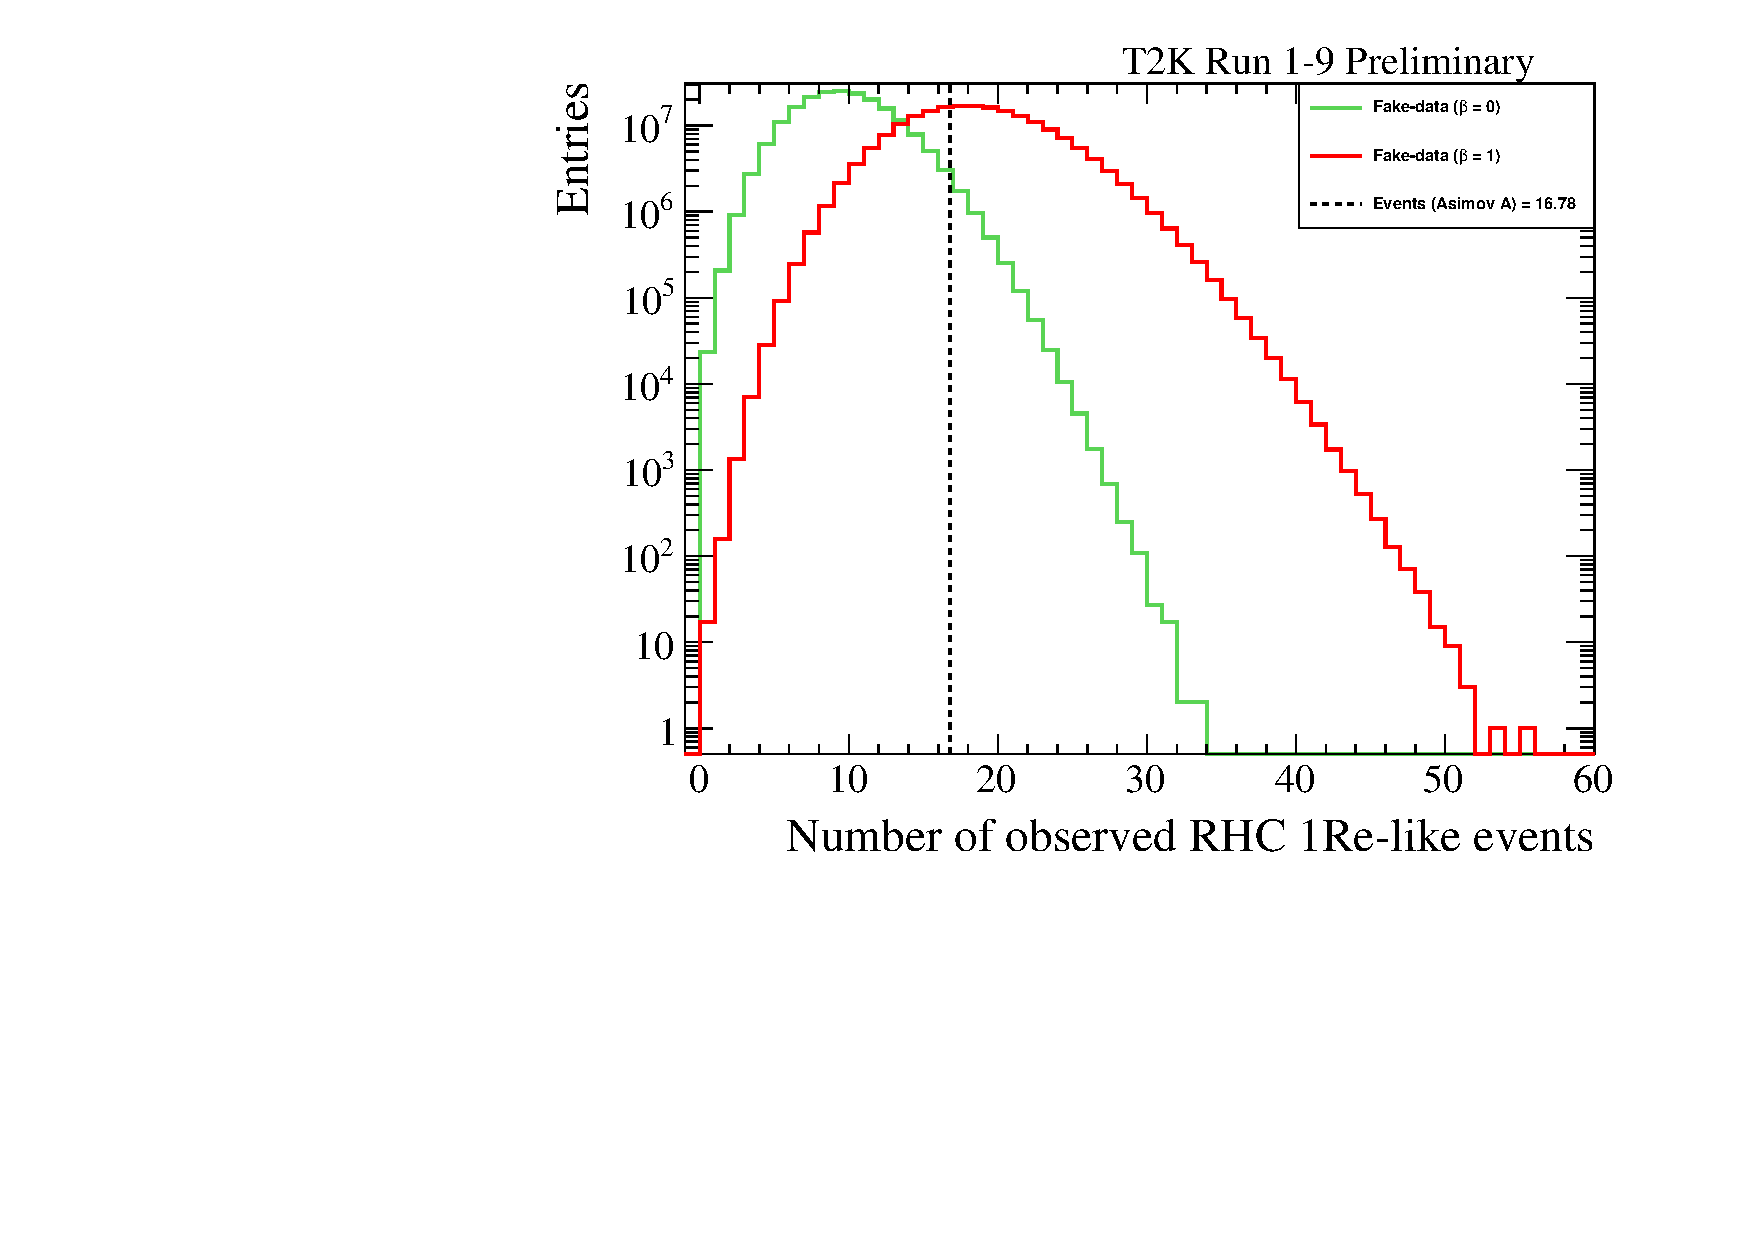
\includegraphics[scale=0.65]{sensitivity/plots_Run1-9d/sensitivity_weighted_2019-01-18/nuebarapp_graphs_nmargtoys_200k_nexp_20k_rate-only_MCsampling_PDG2018_VALOR_Nevents_logscale}
	\caption{The distribution of the total number of events in the antineutrino mode single-ring e-like sample from each of the \NToysFakeDataRateOnly\ toy experiments for both the $\beta = 0$ and $\beta = 1$ hypotheses using full Run 1 - 9 statistics. The distributions were produced using the method outlined in section \ref{sec:method_rate-only} using the Asimov A spectra to calculate the 4-sample likelihood. The dashed line corresponds to the total number of events given by the Asimov A data set.}
	\label{fig:sensitivity_rate-only_Run1-9d}
\end{figure}

\begin{figure}
	\centering
	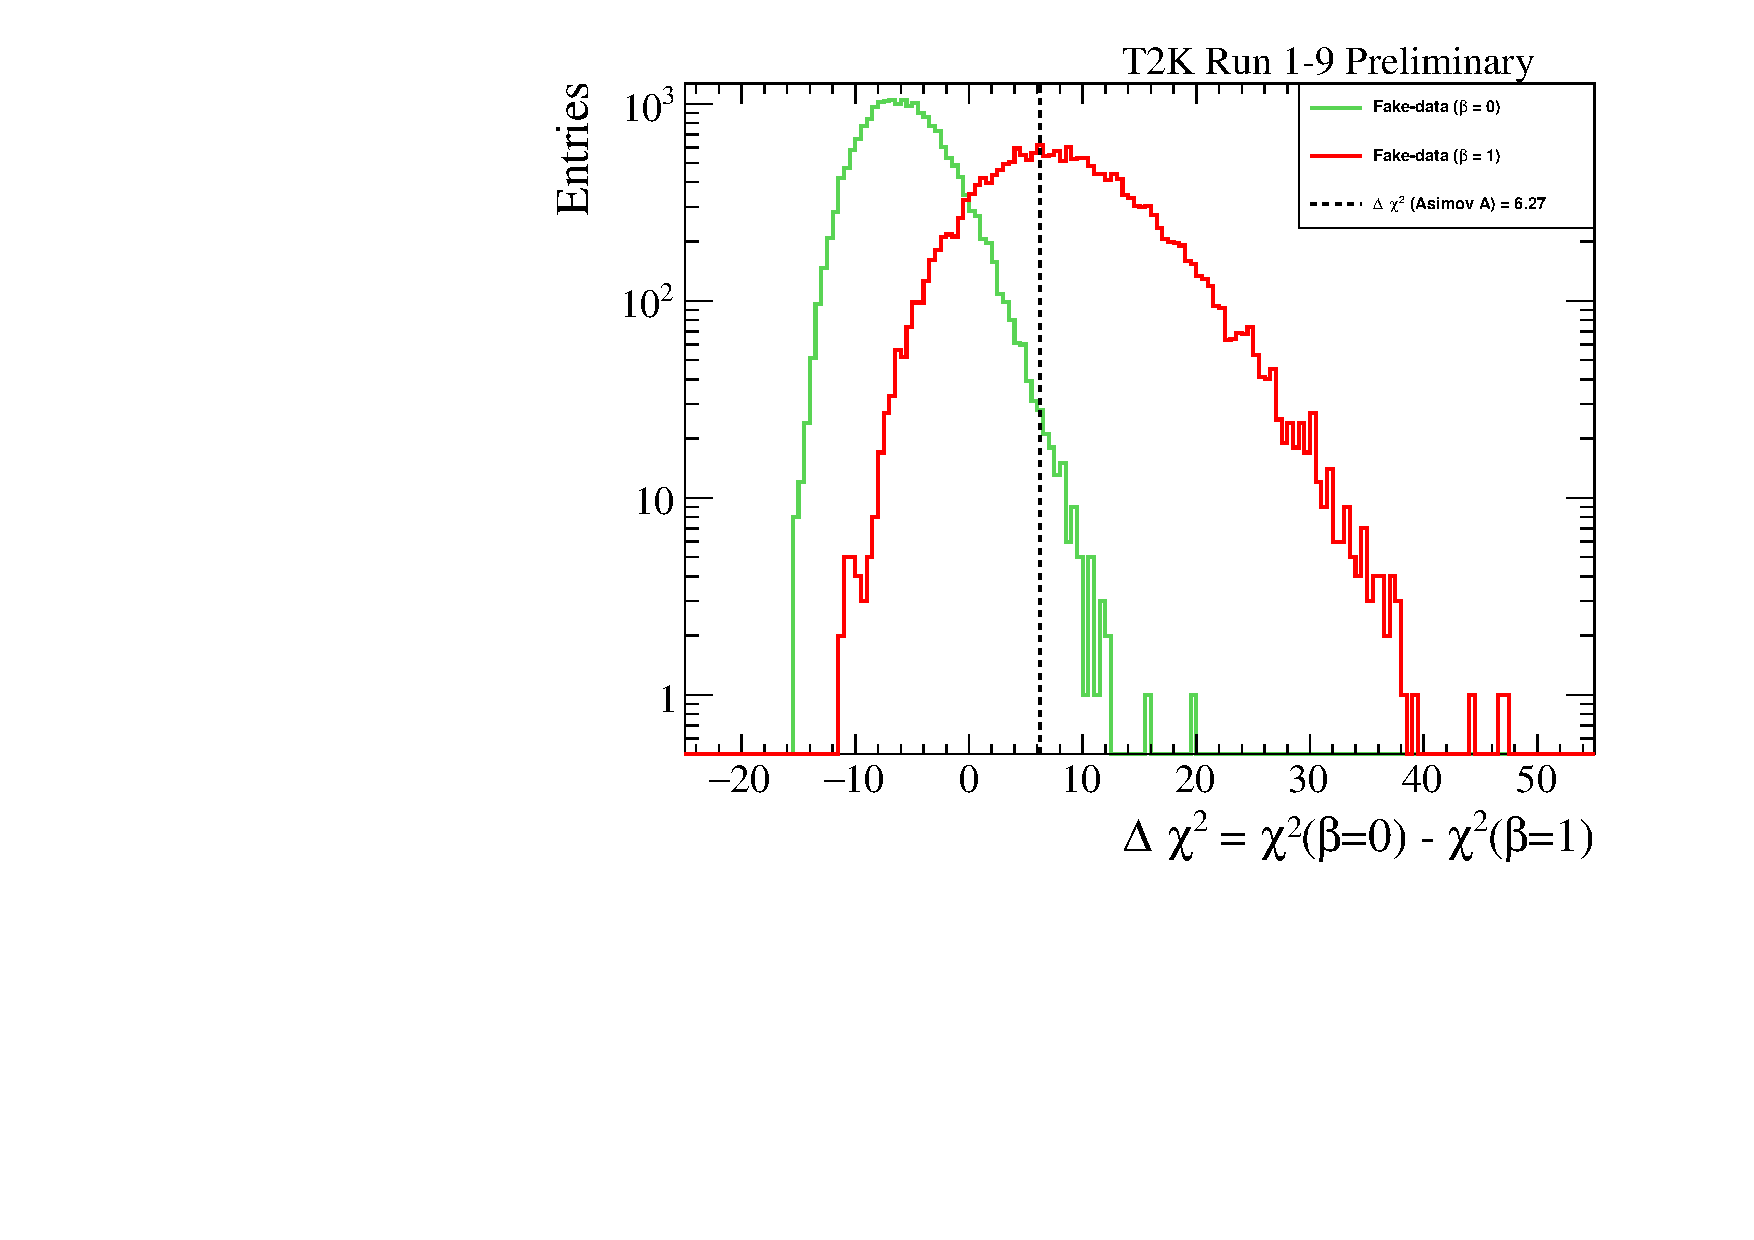
\includegraphics[scale=0.65]{sensitivity/plots_Run1-9d/sensitivity_weighted_2019-01-18/nuebarapp_graphs_nmargtoys_200k_nexp_20k_rate+shape_MCsampling_PDG2018_VALOR_Deltachisq_logscale}
	\caption{The distribution of $\Delta \chi^2$ values from each of the \NToysFakeDataRatePlusShape\ toy experiments for both the $\beta = 0$ and $\beta = 1$ hypotheses using full Run 1 - 9 statistics. The distributions were produced using the method outlined in section \ref{sec:method_rate+shape} using the Asimov A spectra to calculate the 4-sample likelihood. The dashed line corresponds to the $\Delta \chi^2$ value given by the Asimov A data set.}
	\label{fig:sensitivity_rate+shape_Run1-9d}
\end{figure}



\FloatBarrier

\subsection{Results of the $\nueb$ Appearance Analysis} \label{sec:run1-9d_results}

The rate-only and rate+shape p-values for $\nueb$ appearance are performed on the full Run 1-9 data set following the same procedure as in Sec \ref{sec:method}. 1-sided p-values are computed on the right tail of the test statistic expected distribution to exclude $\beta = 0$ and the left tail to exclude $\beta = 1$. Fig \ref{fig:asimova_spectra_all_Run1-9d} shows the data in the 5 Super-K event samples overlaid with the expected event rates for Asimov data set A. In Figs \ref{fig:data_rate-only_Run1-9d} and \ref{fig:data_rate+shape_Run1-9d} the distributions of the test statistic, for rate-only and rate+shape analyses, are shown and compared with the data. The  observed number of events in the antineutrino mode single-ring e-like sample in Super-K was \NskObservedNueBarRunOneNineD. The observed $\Delta \chi^2$ value was \DeltachisqDataRunOneNineD. The p-values resulting from these distributions and test statistic values are shown in Tab \ref{tab:data_pvals_R1-9d}. A comparison to observed p-values produced by the P-theta group is shown in appendix \ref{app:compare_data_valor_ptheta}..

As shown in Tab \ref{tab:data_pvals_R1-9d}, both the rate-only and rate+shape analyses disfavour the $\beta = 0$ hypothesis more than the $\beta = 1$ hypothesis. The Jeffreys scale indicates that the Bayes factor (see eq. \ref{eq:bayes_factor}) of \BayesFactorDataRunOneNineD\ corresponds to a substantial preference for the $\beta = 1$ hypothesis over $\beta = 0$. This preference is in contrast to the earlier Run 1-9c and Run 1-7 analyses, which both had a poor preference for the $\beta = 0$ hypothesis over $\beta = 1$. The comparison between the full Run 1-9 and Run 1-9c analyses is discussed in more detail in Appendix \ref{app:compare_R1-9d_R1-9c}.

\begin{figure}
	\centering
	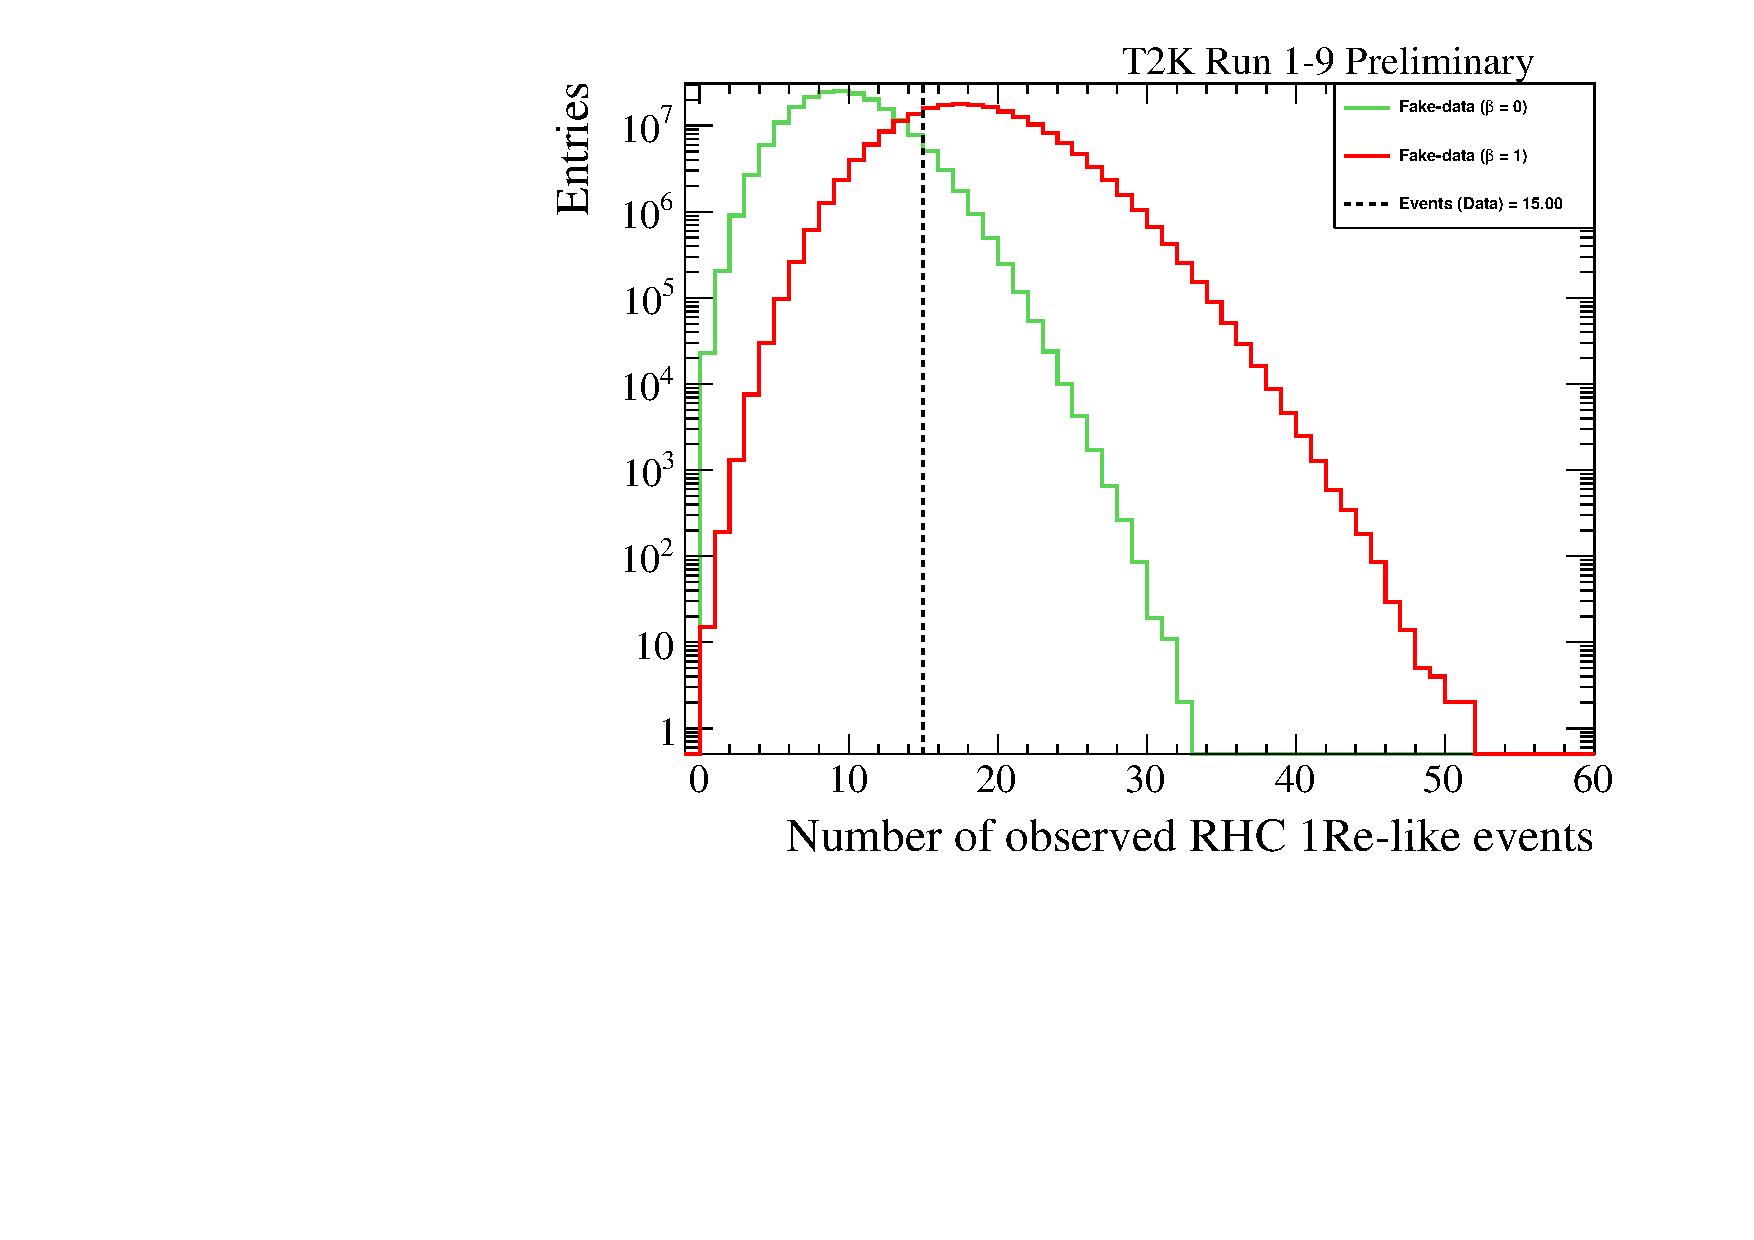
\includegraphics[scale=0.65]{data/Run1-9d/nuebarapp_graphs_nmargtoys=200k_nexp=20k_data_rate-only_MCsampling_VALOR_Nevents_logscale}
	\caption{The distribution of the total number of events in the antineutrino mode single-ring e-like sample from each of the \NToysFakeDataRateOnly\ toy experiments for both the $\beta = 0$ and $\beta = 1$ hypotheses. The distributions were produced using the method outlined in section \ref{sec:method_rate-only} using the Run 1-9d data spectra to calculate the likelihood. The dashed line corresponds to the total number of events given by the Run 1-9d data set.
	}
	\label{fig:data_rate-only_Run1-9d}
\end{figure}

\begin{figure}
	\centering
	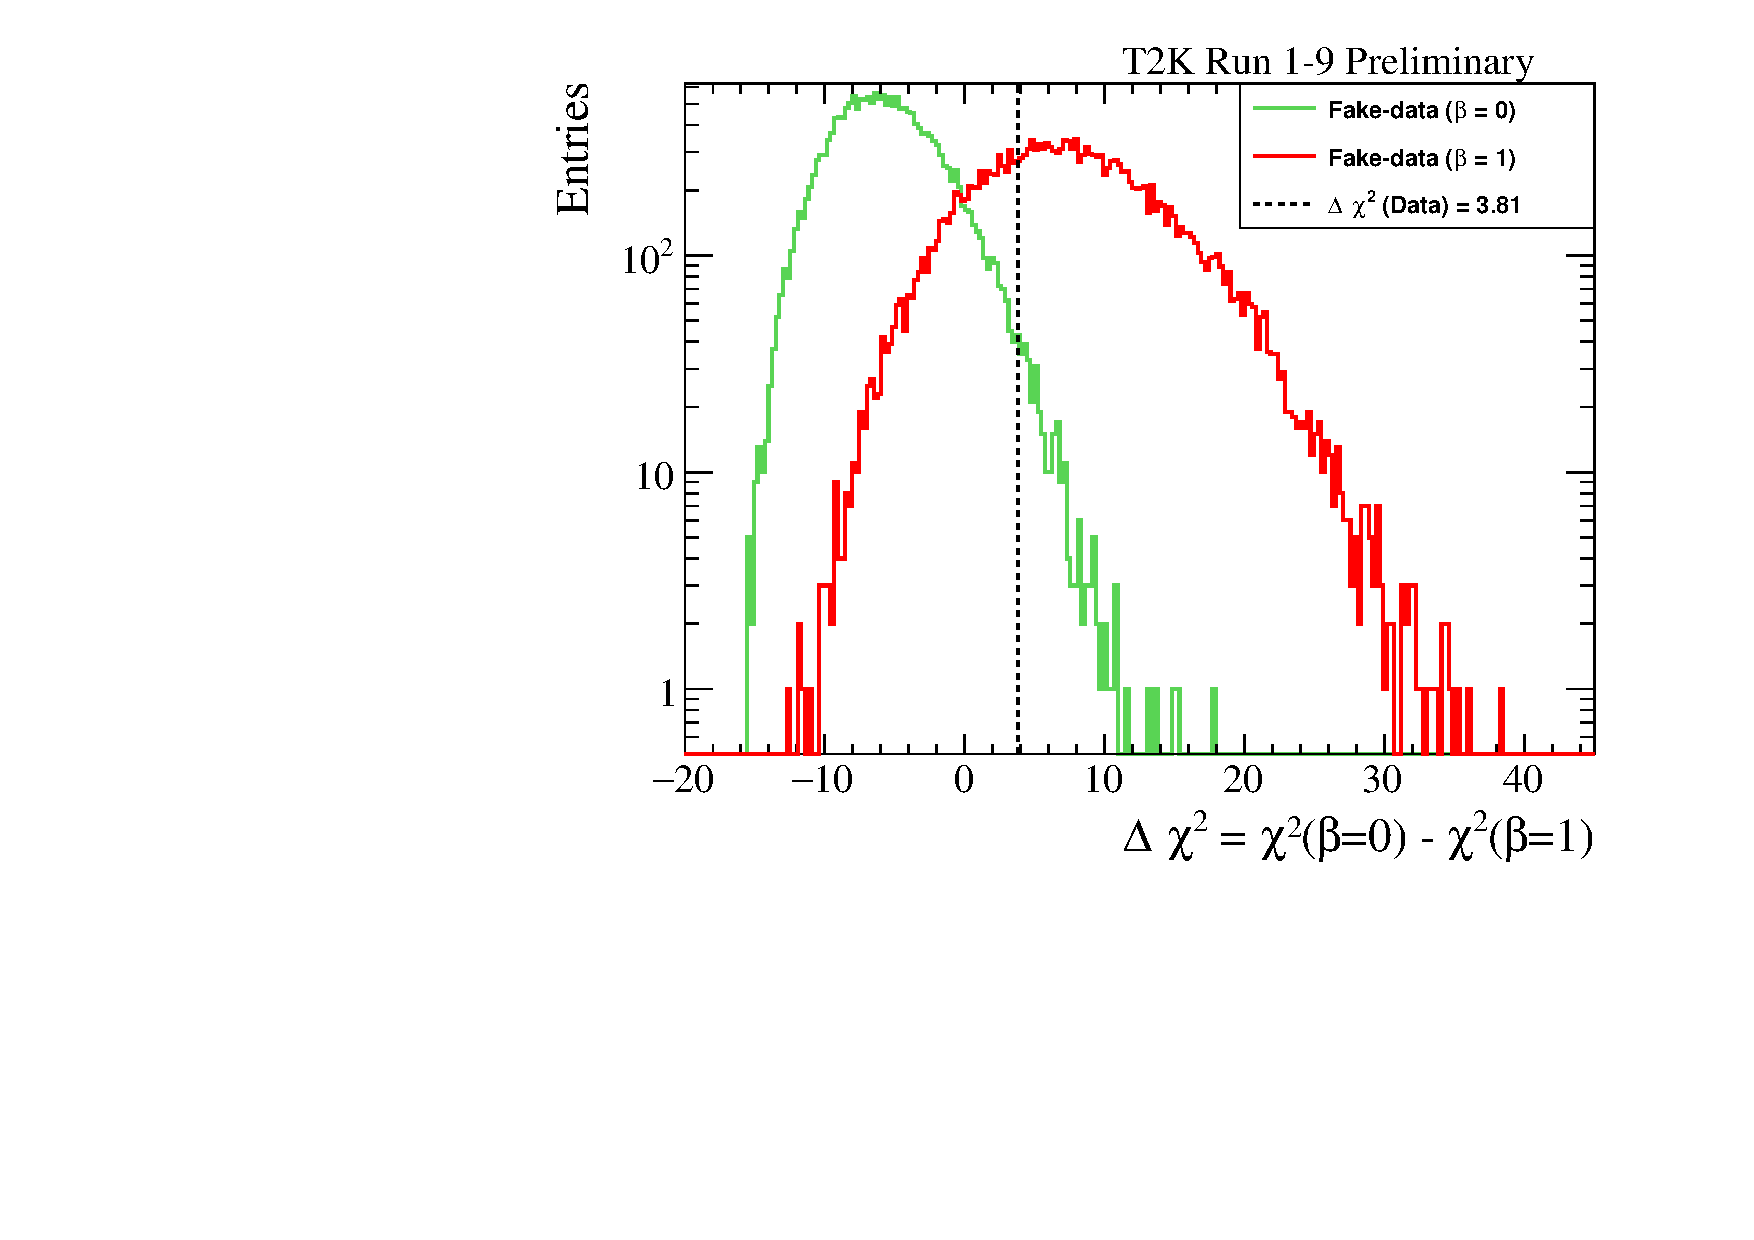
\includegraphics[scale=0.65]{data/Run1-9d/nuebarapp_graphs_nmargtoys=200k_nexp=20k_data_rate+shape_MCsampling_VALOR_Deltachisq_logscale}
	\caption{The distribution of $\Delta \chi^2$ values from each of the \NToysFakeDataRatePlusShape\ toy experiments for both the $\beta = 0$ and $\beta = 1$ hypotheses. The distributions were produced using the method outlined in section \ref{sec:method_rate+shape} using the Run 1-9d data spectra to calculate the likelihood. The dashed line corresponds to the $\Delta \chi^2$ value given by the Run 1-9d data set.
	}
	\label{fig:data_rate+shape_Run1-9d}
\end{figure}

\begin{table}
	\centering
	\begin{tabular}{|c|c|c|c|}
		\hline
		$\beta$				& Analysis		& p-value                		        & $\sigma$ 						           \\
		\hline
		\multirow{ 2}{*}{0} & rate-only		& \pvalRateOnlyBetaZeroDataRunOneNineD  & \sigmaRateOnlyBetaZeroDataRunOneNineD    \\
		\cline{2-4}
			   				& rate+shape	& \pvalRateShapeBetaZeroDataRunOneNineD & \sigmaRateShapeBetaZeroDataRunOneNineD   \\
		\hline
		\multirow{ 2}{*}{1} & rate-only		& \pvalRateOnlyBetaOneDataRunOneNineD   & \sigmaRateOnlyBetaOneDataRunOneNineD     \\
		\cline{2-4}
			   				& rate+shape	& \pvalRateShapeBetaOneDataRunOneNineD  & \sigmaRateShapeBetaOneDataRunOneNineD    \\
		\hline
	\end{tabular}
	\caption{Data p-values and event-rates for the $\beta = 0$ and $\beta = 1$ hypotheses using both the rate-only and rate+shape analyses and the full Run 1-9 dataset}
	\label{tab:data_pvals_R1-9d}
\end{table}


\begin{figure*}[htb]
	\center
	\begin{subfigure}[b]{0.49\textwidth}
		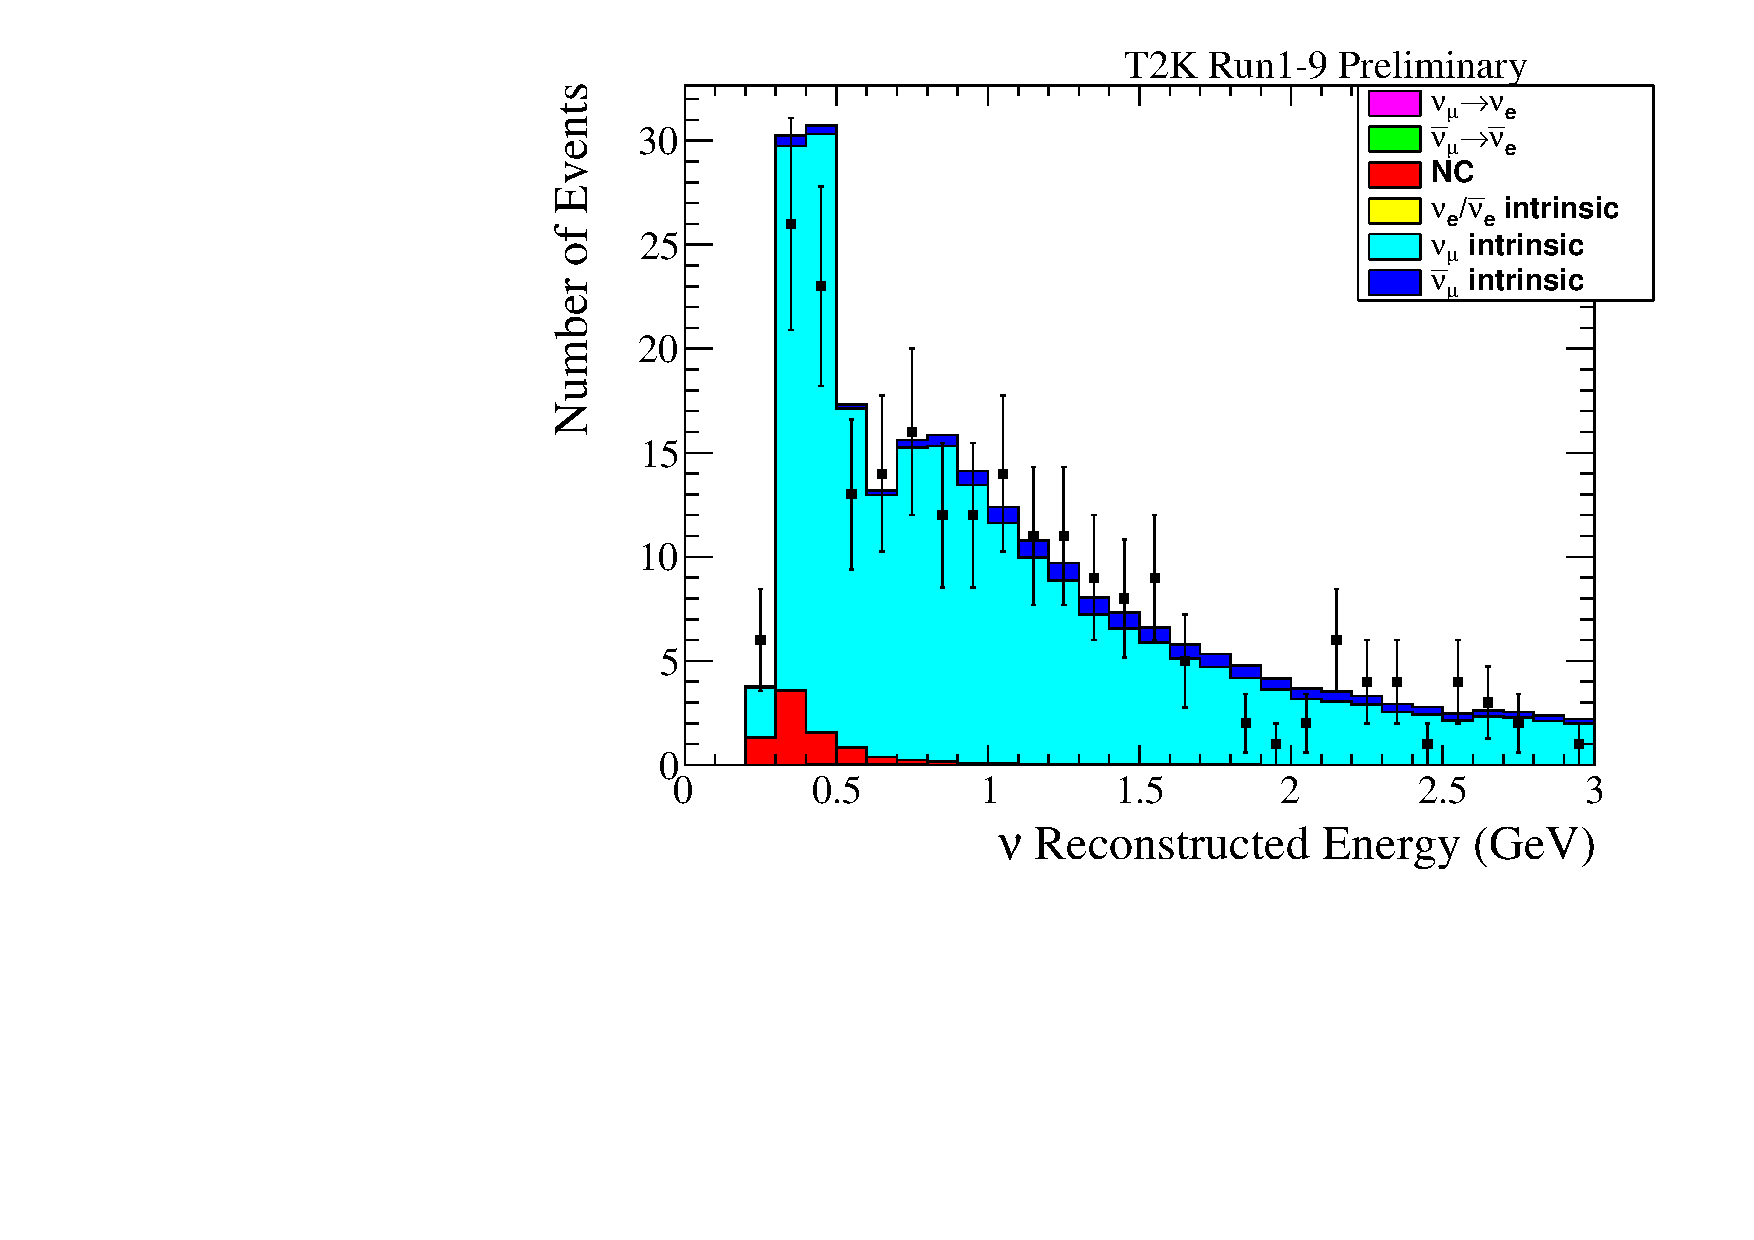
\includegraphics[width=0.9\textwidth]{spectra/Run1-9d/spectrum_AsimovA_1Rmu}
		\caption{Muon-like, neutrino mode}
	\end{subfigure}
	\begin{subfigure}[b]{0.49\textwidth}
		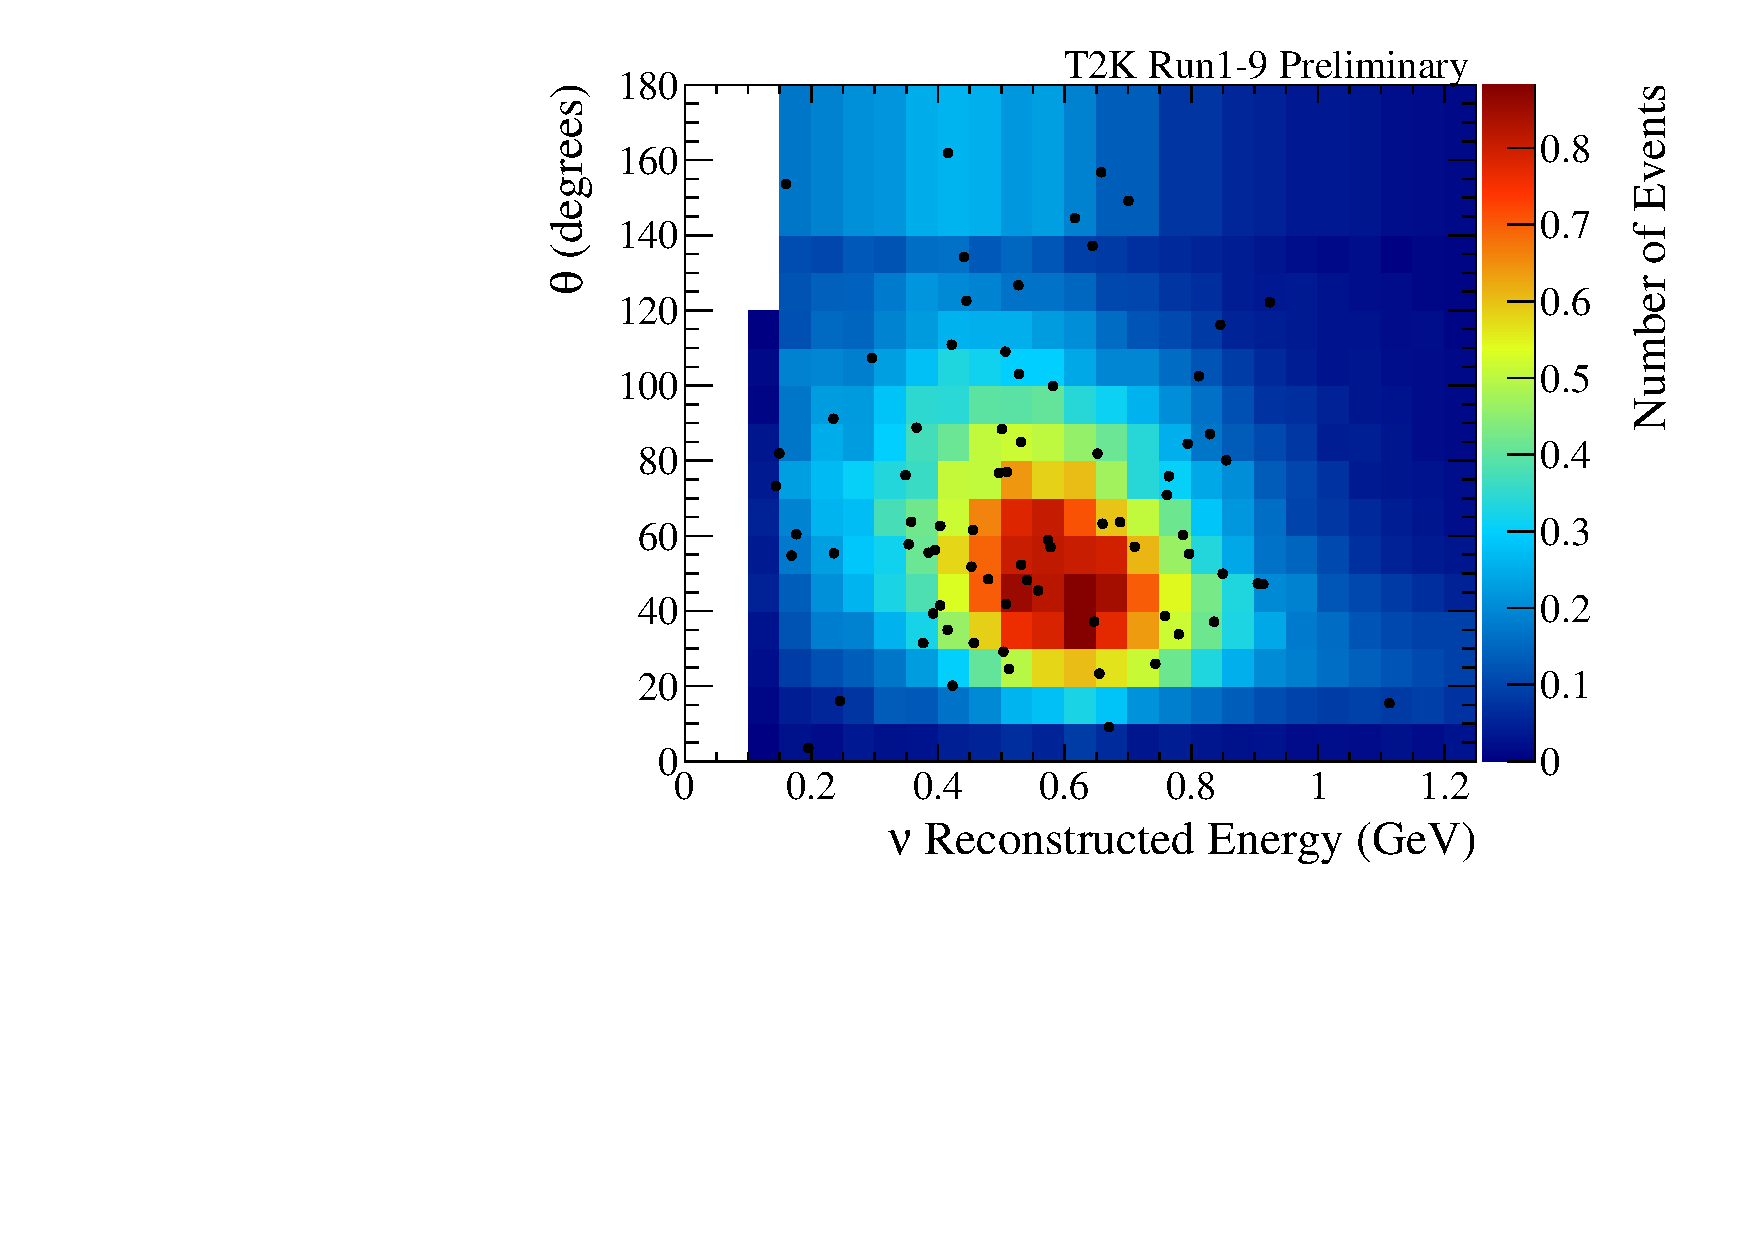
\includegraphics[width=0.9\textwidth]{spectra/Run1-9d/spectrum_AsimovA_1Re}
		\caption{Electron-like, neutrino mode}
	\end{subfigure}
	\begin{subfigure}[b]{0.49\textwidth}
		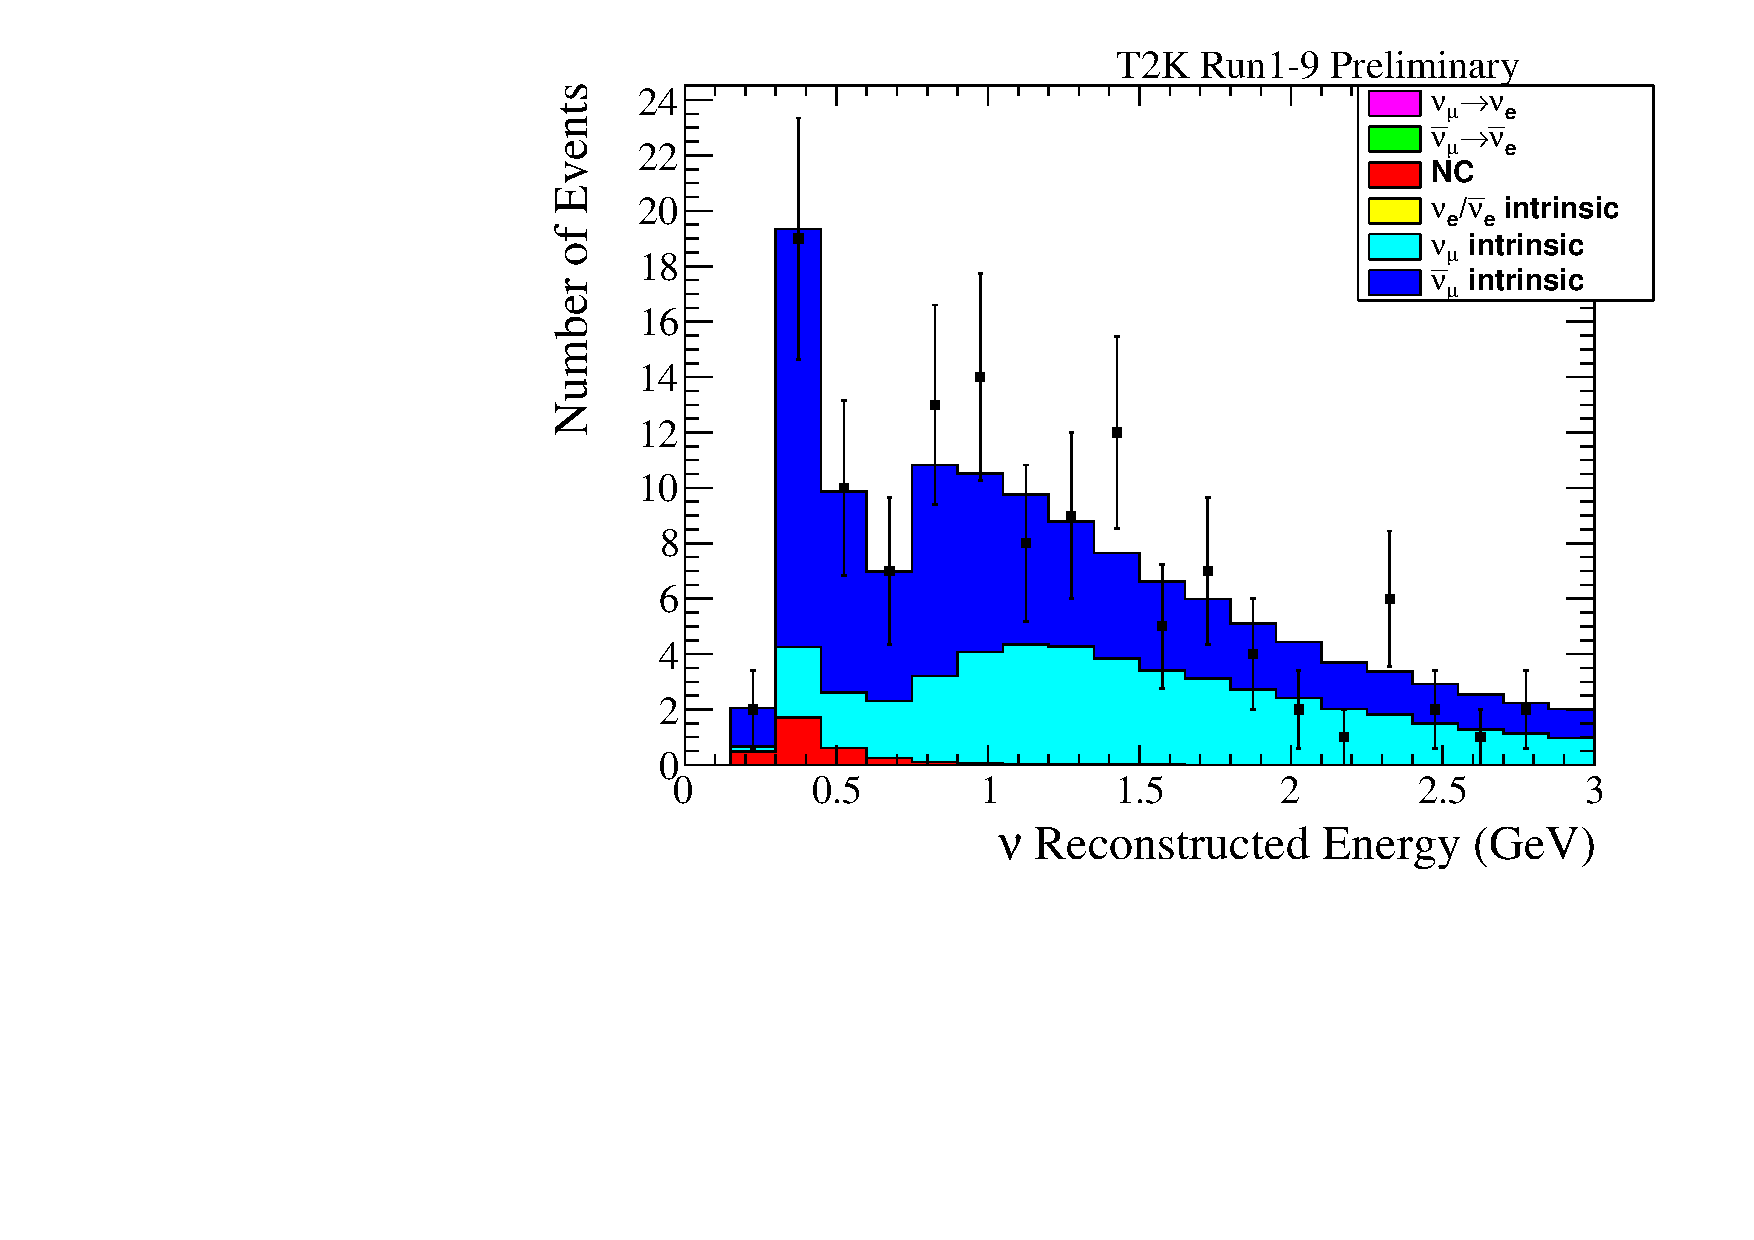
\includegraphics[width=0.9\textwidth]{spectra/Run1-9d/spectrum_AsimovA_RHC1Rmu}
		\caption{Muon-like, antineutrino mode}
	\end{subfigure}
	\begin{subfigure}[b]{0.49\textwidth}
		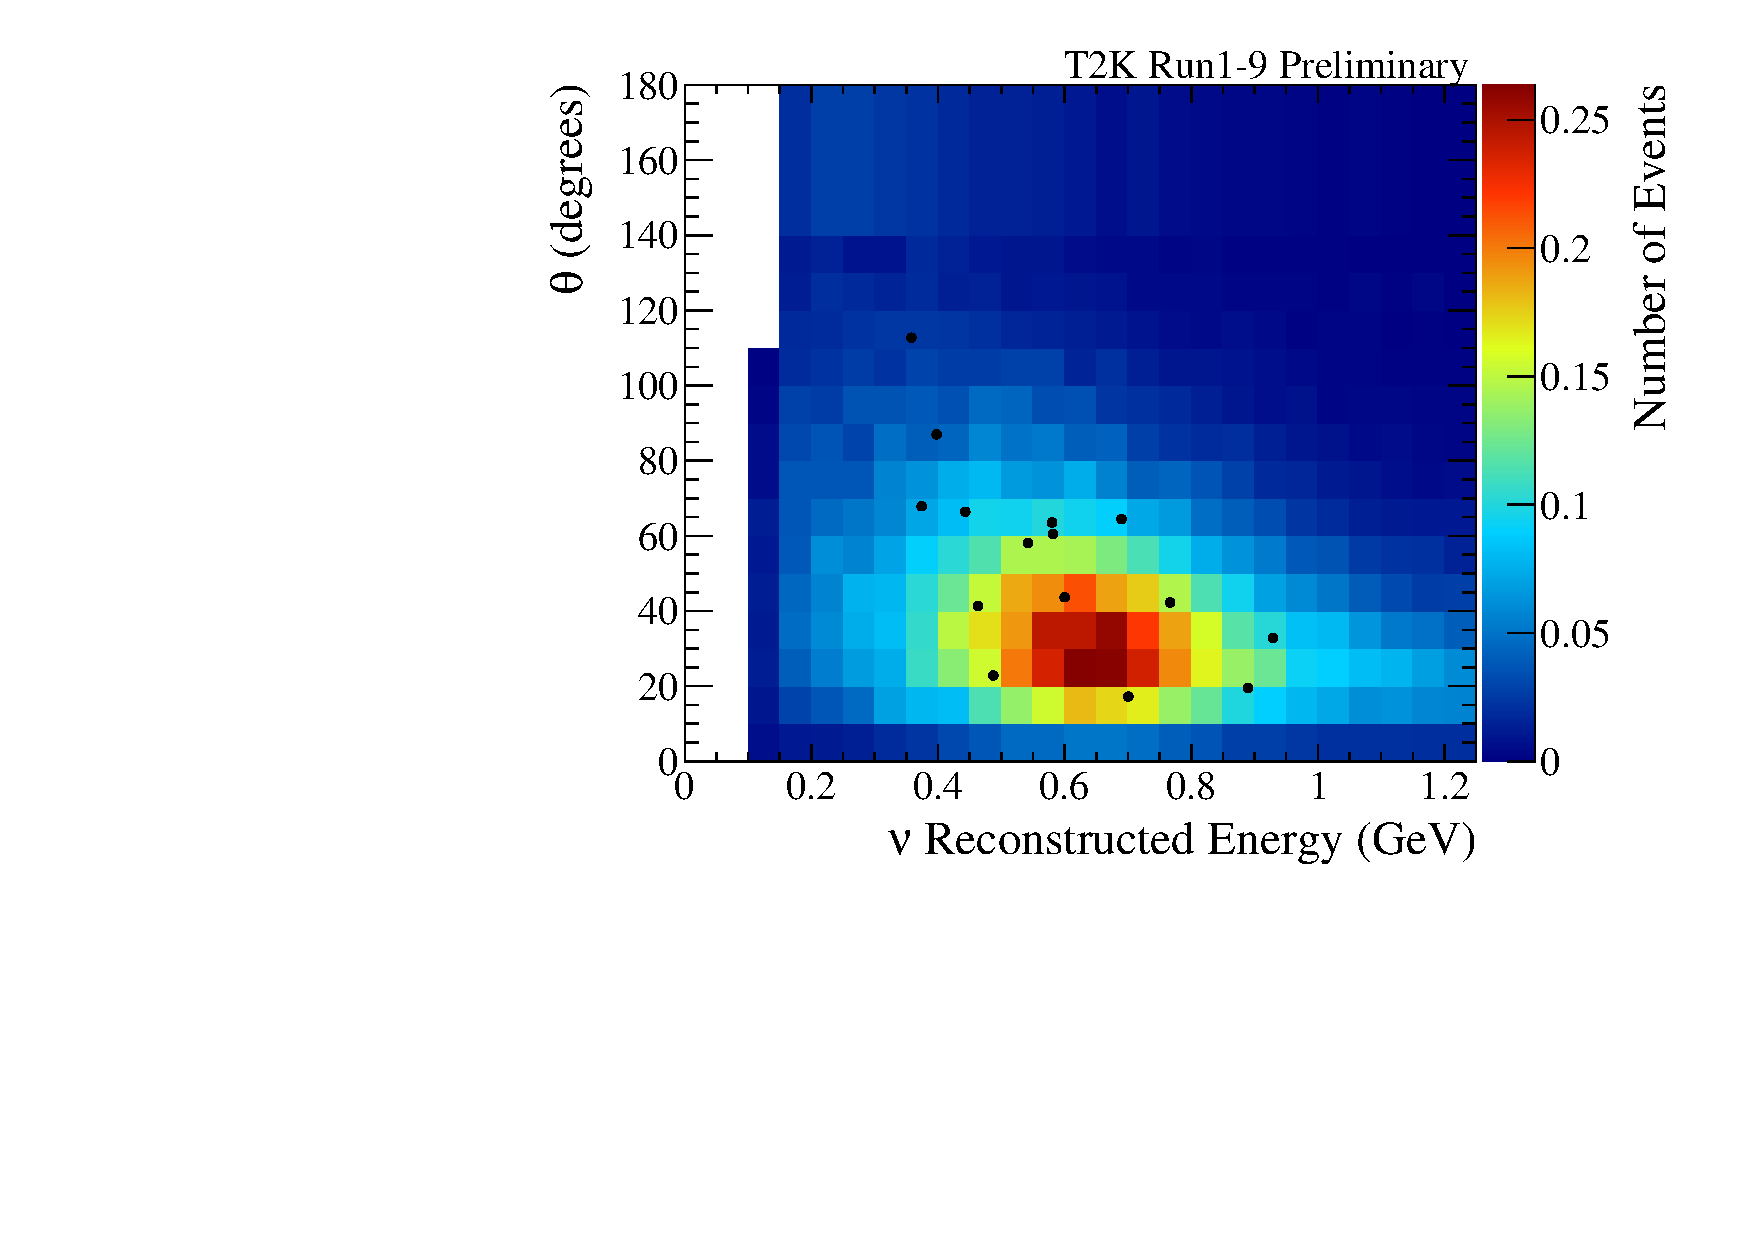
\includegraphics[width=0.9\textwidth]{spectra/Run1-9d/spectrum_AsimovA_RHC1Re}
		\caption{Electron-like antineutrino mode \label{fig:nuebar_tot_spectra_Run1-9d}}
		\label{fig:asimova_spectra_Run1-9d_RHC1Re}
	\end{subfigure}
	\begin{subfigure}[b]{0.49\textwidth}
		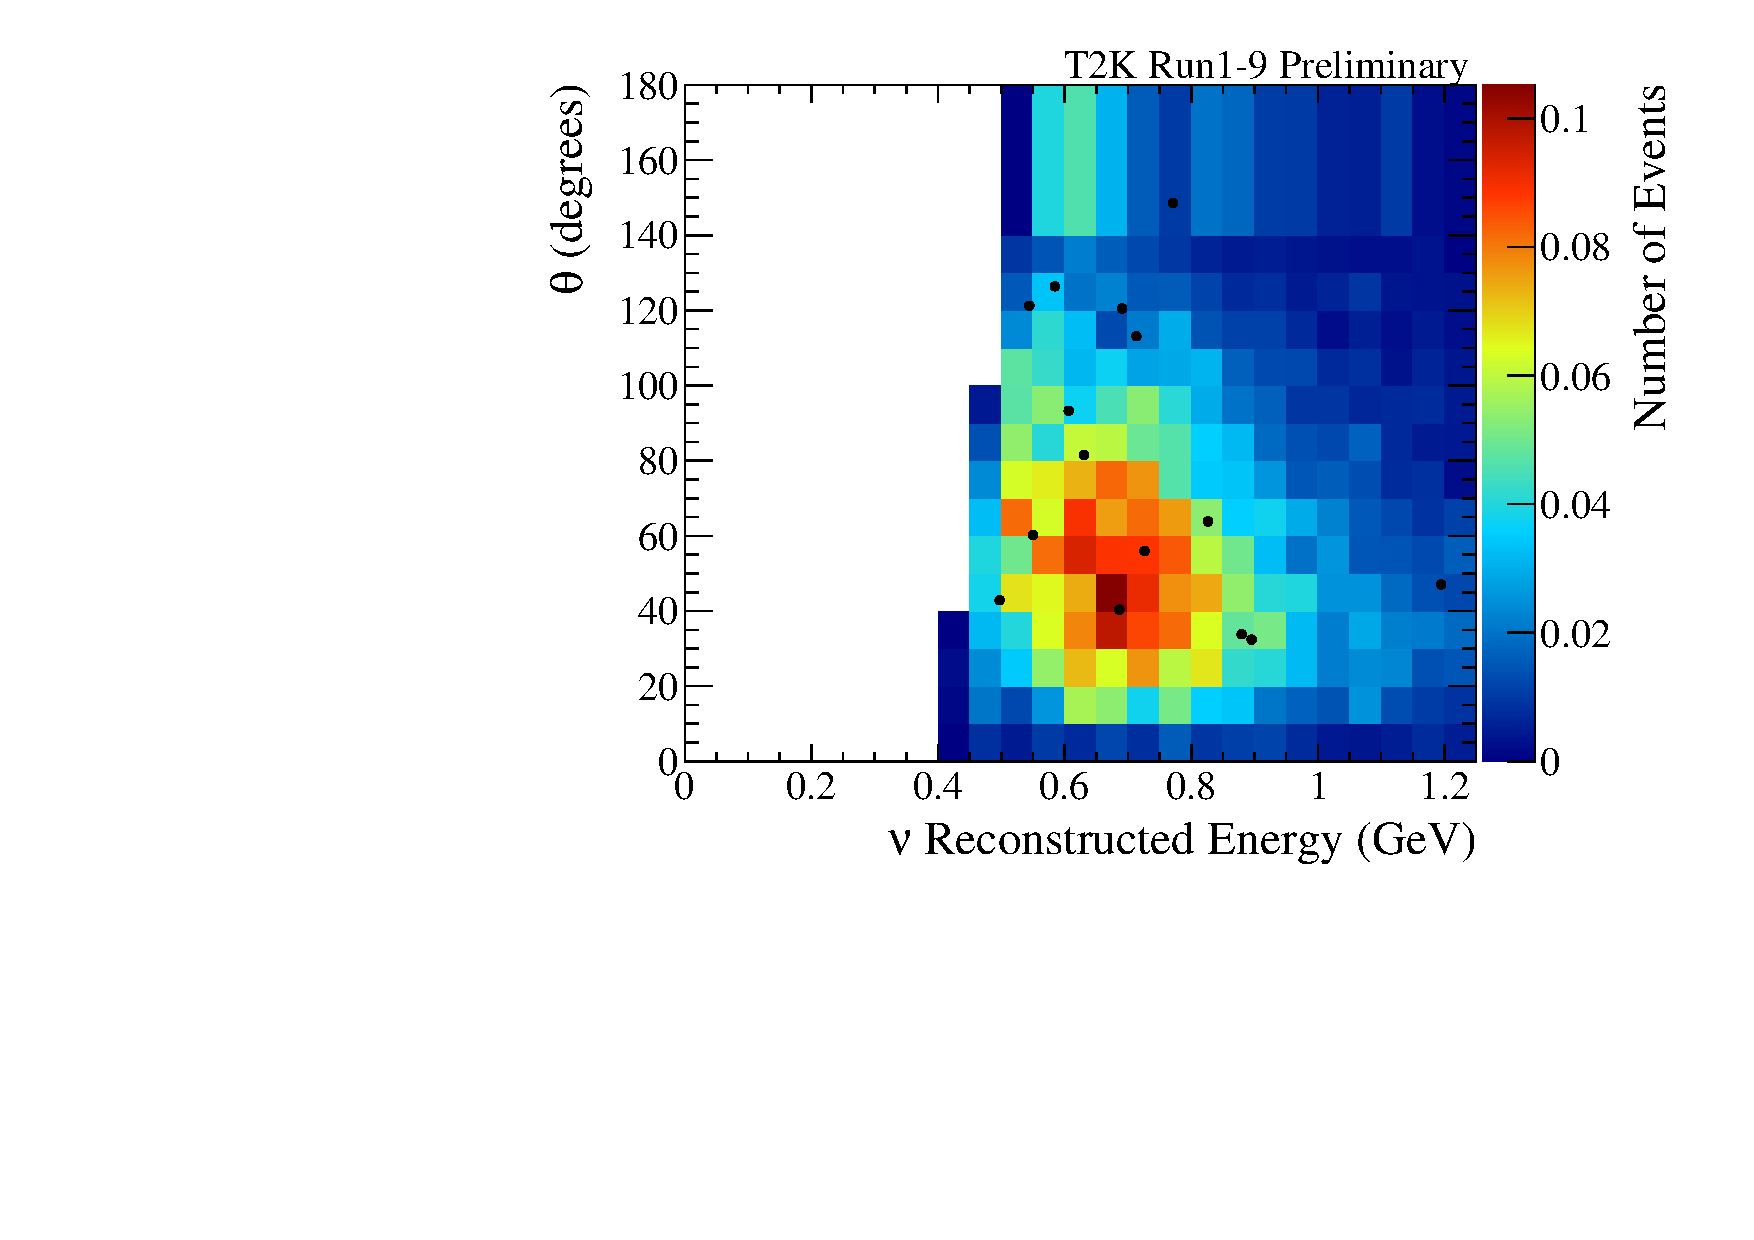
\includegraphics[width=0.9\textwidth]{spectra/Run1-9d/spectrum_AsimovA_MultiRe}
		\caption{\nueCConepi-like, neutrino mode}
	\end{subfigure}
	\caption {
		Predicted Asimov A spectra with Run 1-9 data superimposed. $\mu$-like distributions are a function of the reconstructed neutrino energy, while the $e$-like, including \nueCConepi, distributions are functions of both the reconstructed neutrino energy and the reconstructed angle between the outgoing lepton and the neutrino direction. The distributions correspond to the statistics collected in the full Run 1-9 data set. The spectra are generated with the oscillation parameters corresponding to the Asimov data set A shown in \cref{tab:osc_params_joint_asimovA}.
		%The spectra are generated with the systematic parameters described in \cref{sec:systematics} and the oscillation parameters corresponding to the Asimov data set A shown in \cref{tab:asimov_definition1}.
	}
	\label{fig:asimova_spectra_all_Run1-9d}
\end{figure*}
\clearpage

} % \colour{red}



% References
\clearpage
%
% References
%

% TODO: Find out how to automatically not display unused references

\begin{thebibliography}{9}

\bibitem{OurRun16AntiNueBarAppearanceAnalysis3Flavour}
C.Andreopoulos et al.,
$\nueb$ Appearance Analysis with the 3-Flavour Joint Fit Framework for T2K \TotalPotNuRunOneSix-POT Neutrino \TotalPotNuBarRunOneSix-POT Anti-Neutrino
T2K-TN-296,\\
http://www.t2k.org/docs/technotes/296

\bibitem{OurRun18CC1piJointAnalysis3Flavour}
C.Andreopoulos et al.,
T2K Neutrino and Anti-Neutrino 3-Flavour Joint Analysis of Run 1-9c (\TotalPotNuRunOneNineC-POT $\nu$ \TotalPotNuBarRunOneNineC-POT $\bar{\nu}$) data sets
T2K-TN-327,\\
http://www.t2k.org/docs/technotes/327	

\bibitem{OurRun19JointAnalysis3Flavour}
C.Andreopoulos et al.,
T2K Neutrino and Anti-Neutrino 3-Flavour Joint Analysis of Run 1-9c (\TotalPotNuRunOneNine-POT $\nu$ \TotalPotNuBarRunOneNine-POT $\bar{\nu}$) data sets - Statistical Update
T2K-TN-360,\\
https://t2k.org/docs/technotes/360/run19d/statistical-update

\bibitem{pdg_2014}
K.A. Olive et al. (Particle Data Group 2014 with 2015 update), 
Chin. Phys. C, 38, 090001

\bibitem{pdg_2018}
M. Tanabashi et al. (Particle Data Group), 
Phys. Rev. D 98, 030001 (2018)

t2k neutrino\bibitem{T2KLongPaper}
T2K Collaboration (K.Abe et al.),
Measurement of neutrino oscillation in appearance and disappearance channels by the T2K experiment with 
6.6$\times$10$^{20}$ protons on target 
http://www.t2k.org/comm/pubboard/JournalPapers/oa2014prd/draft3

\bibitem{fiTQunAlgo}
S. Berkman, P. de Perio, A. Konaka, A. Missert, H. Tanaka, S. Tobayama, M. J. Wilking, E. D. Zimmerman
fiTQun: A New Reconstruction Algorithm for Super-K
http://www.t2k.org/docs/technotes/146

\bibitem{PthetaR19cNuebarAppearance}
T.Koga, S.Bienstock, C.Bronner and B.Quilain,
Updated p-theta $\nueb$ appearance search using the T2K RUN1-9 data set,\\
http://www.t2k.org/docs/technotes/353

\bibitem{JeffreysScale}
H. Jeffreys
The Theory of Probability
OUP Oxford
1998

\bibitem{MaCH3NuebarAppearance2015}
A. Kaboth, K. Duffy, R Calland, and D Payne
Analysis of $\nueb$ Appearance using MCMC
T2K-TN-247
http://www.t2k.org/docs/technotes/247 

\bibitem{Asimov} 
G.Cowan, K.Cranmer, E.Gross, O.Vitells,
"Asymptotic formulae for likelihood-based tests of new physics"
arXiv:1007.1727v2

\bibitem{WilksTheorem}
S. Wilks,
The Large-Sample Distribution of the Likelihood Ratio for Testing Composite Hypotheses,
Ann. Math. Statist., 03, 1, 60-62,
https://doi.org/10.1214/aoms/1177732360

\bibitem{Grubbs}
F. Grubbs,
Sample Criteria for Testing Outlying Observations,
Ann. Math. Statist., 03, 1, 27-58,
https://doi.org/10.1214/aoms/1177729885

\bibitem{flux_tuning_Run1-9d}
T. Vladisavljevic,
Full Run 9 T2K Flux Release of  Run 9d (2018/3/9 – 2018/5/31),
https://t2k.org/beam/NuFlux/FluxRelease/13arelease/13av3-tuned-fluxes-for-runs-1-9d-slides

\bibitem{nuebarapp_valor_plenary_run1-9c}
F. Bench,
$\nueb$ Appearance Analysis,
https://t2k.org/meet/collab/201805/talks/fripm/nuebar

\end{thebibliography}



%%% Local Variables:
%%% mode: latex
%%% TeX-master: "../TN327"
%%% End:


%Appendices
\clearpage
\begin{appendices}
	\crefalias{section}{appsec}
	\section{Optimisation of Oscillation Parameter Priors}\label{app:priors}
When generating fake-data toys that are {\color{red} constrained} by the \RunPeriod real-data (see section \ref{sec:method}), it was found that the amount of CPU time required to generate these toys was $\sim 80\times$ the CPU time required to generate toys {\color{red} constrained} by Asimov A fake-data.

The reason for this is that the constraints on the oscillation parameters given by the \RunPeriod data are substantially stronger than the Asimov A constraints \cite{OurRun18CC1piJointAnalysis3Flavour}. This results in a larger fraction of the oscillation parameters being generated at more unlikely values and therefore the mean probability of accepting each fake-data toy decreased by a factor of 138. 

The large increase in CPU time meant that the toy generation process would require an unreasonably large amount of time and the majority of fake-data toys generated would be immediately rejected. In order to increase the efficiency of the fake-data toy generation process, the oscillation parameter priors ranges were reduced from the ranges used to generate marginalization and fake-data toys in the \RunPeriod joint analysis \cite{OurRun18CC1piJointAnalysis3Flavour}, these ranges will be referred to as the \emph{nominal priors} and are shown in the \emph{Range for marginalisation toys} column of Tab \ref{tab:osc_param_priors_nuebarapp_optimised}.

By restricting the range of the each oscillation parameter prior to the region close to the \RunPeriod best-fit point \cite{OurRun18CC1piJointAnalysis3Flavour}, a larger fraction of fake-data toys generated will have a higher likelihood compared to toys generated using the nominal prior ranges (referred to as the \emph{nominal set}), resulting in a reduction in the required CPU time. However, there is a danger that by reducing the prior range, a toy that would have been accepted from the nominal set would no longer be generated and so would be excluded from the new set of accepted toys. This could cause a change in the measured p-values, which would be undesirable.

To quantify this effect on the p-values, the maximum possible change in p-value is calculated as follows. Equations \ref{eq:pval_right} and \ref{eq:pval_left} for the calculation of the p-value can be re-written as

\begin{equation} \label{eq:pval_ntoys}
\textrm{p-value} = p = \frac{n}{N}
%\frac{\textrm{number of toys in tail of interest}}{\textrm{total accepted toys}}
\end{equation}

Where $n$ is the number of accepted toys in the tail of interest and $N$ is the total number of accepted toys in the test-statistic distribution. At worst, all toys that were excluded from the nominal set could have been in the tail of interest, but when using the reduced prior, these excluded toys would have been re-thrown (to keep the total number of accepted toys constant). At worst, all of these re-thrown toys would be outside of the tail of interest (or vice-versa). Using equation \ref{eq:pval_ntoys}, this gives a maximum possible p-value change, $|\Delta p|_{\textrm{max}}$ of

\begin{equation} \label{eq:dpmax}
|\Delta p|_{\textrm{max}} 
= \left| p_{\textrm{nominal}} - p \right|
= \left| \frac{n_{\textrm{nominal}}}{N} - \frac{n_{\textrm{nominal}} \pm n_{\textrm{excluded}}}{N} \right|
= \frac{n_{\textrm{excluded}}}{N}
\end{equation}

Therefore, by reducing the prior ranges successively for a number of oscillation parameters and calculating $|\Delta p|_{\textrm{max}}$ for various potential prior ranges, the CPU time required can be minimised whilst keeping $|\Delta p|_{\textrm{max}}$ smaller than the minimum error on the p-values observed in the Asimov A sensitivity study (see section \ref{sec:sensitivity}), which was \minPvalErrorAsimovA. This is demonstrated for a number of different $\sin^2 \theta_{23}$ prior ranges in Tab \ref{tab:vary_prior_mixing23}, from which a new prior of $[0.42, 0.62]$ is chosen. Using the same method with this new prior range, $\Delta m^2_{23}$ and subsequently $\delta_{CP}$ have their prior ranges optimised, the results of which are shown in Tab \ref{tab:vary_prior_all}.

\begin{table}[H]
\centering
\begin{tabular}{| c | c | c | c |}
	\hline
	$\sin^2 \theta_{23}$          & Toys excluded from the nominal  & Maximum possible    & CPU time \\
	Prior range                   & set (of 20,000 accepted toys)   & p-value change      & (current / nominal) \\
	\hline
	$[ 0.300 , 0.700 ]$ (nominal) & 0                                   & 0               & 1       \\
	$[ 0.355 , 0.680 ]$           & \SI{1.32e-08}{}                     & \SI{6.64e-13}{} & 0.85\\%0.64 \\
	$[ 0.375 , 0.660 ]$           & \SI{2.40e-5}{}                      & \SI{1.20e-9}{}  & 0.71\\%0.58\\
	$[ 0.390 , 0.650 ]$           & \SI{7.34e-4}{}                      & \SI{3.97e-8}{}  & 0.66\\%0.54     \\
	$[ 0.410 , 0.625 ]$           & 1.25                                & \SI{6.24e-5}{}  & 0.55\\%0.50     \\
	$[ 0.420 , 0.620 ]$           & 5.04                                & \SI{2.52e-4}{}  & 0.52\\%0.47   \\
	$[ 0.430 , 0.610 ]$           & 52.5                                & \SI{2.62e-3}{}  & no data  \\
	$[ 0.440 , 0.605 ]$           & 134                                 & \SI{6.74e-3}{}  & no data  \\
	\hline
\end{tabular}
\caption{
Maximum possible effect on the p-values obtained by varying the $\sin^2 2 \theta_{23}$ prior range used to generate toys to fill the test-statistic distributions. \emph{Toys excluded from the nominal set} are the number of toys that would have been accepted (using the MC sampling method) if the nominal prior range had been used but lie outside of the range of the tighter prior under consideration. These are calculated assuming 20,000 accepted toys will be generated.
%toys generated using oscillation parameter priors set to their nominal ranges.
}
\label{tab:vary_prior_mixing23}
\end{table}
\begin{table}[H]
\centering
\begin{tabular}{| c | c | c | c | c |}
	\hline
	Parameter            & Nominal Prior  & Optimised Prior               & Maximum possible           & CPU time \\
	                     &                &                               & p-value change $(10^{-4})$ & (Optimised / Nominal) \\
	\hline
	$\sin^2 \theta_{23}$ & $[0.30, 0.70]$ & $[0.42, 0.62]$                & $2.5$                      & 0.52 \\
	$\Delta m^2_{23}$    & $[2.30, 2.70]$ & $[2.30, 2.65]$                & $4.6$                      & 0.45 \\
	$\delta_{CP}$        & $[-\pi, \pi]$  & $[-\pi, 1.1]$ \& $[1.8, \pi]$ & $7.8$                      & 0.39 \\
	\hline
\end{tabular}
\caption{
	Optimised priors for the oscillation parameters that are randomised according to flat prior probability distributions. The maximum possible effect on the p-values and the expected reduction on CPU time are shown. These are calculated assuming 20,000 accepted toys will be generated.
}
\label{tab:vary_prior_all}
\end{table}

% with Dmsq23 optimisation, cpu time / nominal = 0.4375
% with deltaCP optimisation, cpu time / nominal = awaiting data

% expected CPU time / nominal for:
% mixing23 = 0.52 %0.34
% dm23sq = 0.45 %0.31
% dcp = 0.39 %0.28

% Observed CPU time / nominal (with 90k total toys, so low statistics on the accepted toys) for:
% mixing23 = 0.47
% dm23sq = 0.44
% dcp = 0.27

% Observed acceptance rate (from 6490719 total toys with 1776 accepted toys) = 0.0002736214585780096. So for 20,000 accepted toys, need 73093682.43243243 total toys
% Expected number of nominal toys required is 180106303.473, so actual optimised CPU time / expected nominal CPU time is 0.41, which is close to the predicted 0.39, so my calculations are justified

{\color{red} 

\subsection{Updated Priors for the Full Run 1-9 Analysis}\label{app:priors_Run1-9d}
As shown by the full Run 1-9 sensitivity study (see Tab \ref{tab:sensitivity_AsimovA_R1-9d}), the smallest p-value error has reduced from \minPvalErrorAsimovA\ to \minPvalErrorAsimovABetaZeroRunOneNineD\ so the prior ranges must be changed accordingly. The $\Delta m^2_{23}$ prior was changed from $[2.30, 2.70]$ to $[2.30, 2.67]$ to decrease the maximum possible change in p-value to $\SI{5.30e-4}{}$, which is equal to the min. p-value error. This increases the required CPU time to $41\%$ of the nominal time. The other to priors were not changed from the values in Tab \ref{tab:vary_prior_all}.

} % \colour{red}

% Run 1-9d priors: --prior-mixing12 gaus,0.846,0.021,sinsq2th --prior-mixing23 flat,0.42,0.62,sinsqth --prior-mixing13 gaus,0.0830,0.0031,sinsq2th --prior-dmsq12 gaus,7.53E-5,0.18E-5 --prior-dmsq23 flat,2.3E-3,2.67E-3 --prior-deltacp flat,-4.4831853072,1.1
%For beta = 0, the combined prior changes for all parameters gives a total maximum change in p-value of 5.30e-4 (contributions: 5.51e-05 from mixing23, 1.16e-4 from deltacp and  3.59e-4 from dmsq)
%For beta = 1, the combined prior changes for all parameters gives a total maximum change in p-value of 5.69e-4 (contributions: 5.70e-05 from mixing23, 1.34e-4 from deltacp and  3.78e-4 from dmsq)


	\section{p-value Stability}\label{app:pval_stability}
In order to assess whether the number of fake-data toys used is sufficient, the stability of the generated p-values is assessed. This is done by generating four independent sets of \NToysFakeDataRatePlusShape\ AsimovA-{\color{red}constrained} toys and calculating their corresponding rate-only and rate+shape p-values, following the method described in section \ref{sec:method}, and shown in Tab \ref{tab:pval_stability}. Qualitatively, these p-values are roughly consistent with each other as the observed variation is not large enough to change the conclusions made; however, as more data is collected it is possible that the variation in p-value could affect the conclusions made on the physics, for example if the p-value was close to the threshold for discovery. Therefore, it is important for future analyses to ensure that enough toys are used to keep the variation in p-value small enough that the p-values are quantitatively consistent with each other.

Additionally, the p-value is dependant on the ensemble of nuisance parameters used. As each of the four sets of fake-data toys correspond to different sets of \NToysFakeDataRatePlusShape\ nuisance parameter throws, the p-values will not be drawn from the same underlying distribution and therefore may not be directly comparable, although the size of this effect is currently unknown. Therefore studies need to be performed during future analyses to characterise this effect.

\begin{table}
\centering
\begin{tabular}{| c | c | c | c | c |}
\hline
\multirow{2}{*}{Set} & \multicolumn{2}{|c|}{Rate-only p-value}  & \multicolumn{2}{|c|}{Rate+shape p-value} \\
\cline{2-5}
   				     & $\beta = 0$          & $\beta = 1$       & $\beta = 0$          & $\beta = 1$       \\
\hline
1                    & $0.0364 \pm 0.001$   & $0.387 \pm 0.003$ & $0.0128 \pm 0.0008$  & $0.426 \pm 0.002$ \\
2                    & $0.0363 \pm 0.001$   & $0.386 \pm 0.003$ & $0.0134 \pm 0.0008$  & $0.420 \pm 0.002$ \\
3                    & $0.0363 \pm 0.001$   & $0.386 \pm 0.003$ & $0.0125 \pm 0.0008$  & $0.425 \pm 0.002$ \\
4                    & $0.0362 \pm 0.001$   & $0.387 \pm 0.003$ & $0.0148 \pm 0.0009$  & $0.421 \pm 0.002$ \\
\hline
\end{tabular}
\caption{
	p-values obtained from four separate sets of \NToysFakeDataRatePlusShape\ AsimovA-{\color{red}constrained} fake-data toys
}
\label{tab:pval_stability}
\end{table}





{\color{red} 

\subsection{Improved p-value Stability Study using the Full Run 1-9 Sensitivity}\label{app:pval_stability_Run1-9d}

To assess the stability of the p-values in a more quantitative manner and with a larger set of p-values, the p-value stability study  was redone during the full Run 1-9 analysis using the earlier true value of $\sin^2(\theta_{13})$ in Tab \ref{tab:osc_params_joint_asimovA}. Now the stability of the p-values for each test statistic and value of $\beta$ are assessed by searching for outliers in sets of 10 independent p-values. Whether a p-value is considered an outlier is determined by applying a two-sided Grubbs' test for outliers, which makes use of Student's t-distribution to search for outliers in an approximately normal data set \cite{Grubbs}:

For each test statistic and value of $\beta$, $N=10$ independent sets of \NToysFakeDataRatePlusShape\ AsimovA-constrained toys are generated and fluctuated (marginalised) to obtain rate-only (rate+shape) p-values, $p$.

Grubbs' test statistic, $G$ is defined as

\begin{equation} \label{eq:Grubbs_statistic}
G = \frac{ ^{ \quad \text{max}}_{i=1,...,N} |p_i - \bar{p}| }{ s }
\end{equation}

Where $\bar{p}$ is the mean p-value and $s$ is the sample standard deviation of the p-values calculated with the tested p-value, $p_i$, removed.

The null hypothesis of Grubbs' test, $\text{H}_{0}$, is that none of the p-values are outliers. The alternative hypothesis, $\text{H}_{\text{a}}$, is that there is exactly one outlier. $\text{H}_{0}$ is then rejected and $p_i$ is considered to be an outlier if the following condition is met:

\begin{equation} \label{eq:Grubbs_condition}
G > \frac{N - 1}{N} \sqrt{\frac{ t^2_{\alpha/(2N), N-2} }{ N - 2 + t^2_{\alpha/(2N), N-2} }}
\end{equation}

Where $t^2_{\alpha/(2N), N-2}$ is the critical value of Student's t-distribution with $N-2$ d.o.f and significance level $\alpha$.

The p-values for each of the 10 toy sets, calculated for both rate-only and rate+shape analyses under both the $\beta = 0$ and $\beta = 1$ hypotheses, are shown in Tab \ref{tab:pval_stability_Run1-9d_values}. The most extreme p-values from this table are assessed in Tab \ref{tab:pval_stability_Run1-9d} and it is shown that, at a significance level of $\alpha = 0.05$, none of the p-values are considered to be outliers. Therefore \NToysFakeDataRatePlusShape\ fake data toy sets is considered to be sufficient at this significance level.

\begin{table}
\centering
\begin{tabular}{| c | c | c | c | c |}
\hline
\multirow{2}{*}{Set} & \multicolumn{2}{|c|}{Rate-only p-value}     & \multicolumn{2}{|c|}{Rate+shape p-value} \\
\cline{2-5}
   				     & $\beta = 0$           & $\beta = 1$         & $\beta = 0$           & $\beta = 1$         \\
\hline
1                    & $ 0.0101 \pm 0.0007 $ & $ 0.463 \pm 0.004 $ & $ 0.0035 \pm 0.0004 $ & $ 0.436 \pm 0.004 $ \\
2                    & $ 0.0102 \pm 0.0007 $ & $ 0.463 \pm 0.004 $ & $ 0.0036 \pm 0.0004 $ & $ 0.438 \pm 0.004 $ \\
3                    & $ 0.0102 \pm 0.0007 $ & $ 0.463 \pm 0.004 $ & $ 0.0038 \pm 0.0004 $ & $ 0.439 \pm 0.004 $ \\
4                    & $ 0.0102 \pm 0.0007 $ & $ 0.464 \pm 0.004 $ & $ 0.0038 \pm 0.0004 $ & $ 0.440 \pm 0.004 $ \\
5                    & $ 0.0102 \pm 0.0007 $ & $ 0.464 \pm 0.004 $ & $ 0.0041 \pm 0.0005 $ & $ 0.440 \pm 0.004 $ \\
6                    & $ 0.0103 \pm 0.0007 $ & $ 0.465 \pm 0.004 $ & $ 0.0041 \pm 0.0005 $ & $ 0.440 \pm 0.004 $ \\
7                    & $ 0.0103 \pm 0.0007 $ & $ 0.465 \pm 0.004 $ & $ 0.0042 \pm 0.0005 $ & $ 0.441 \pm 0.004 $ \\
8                    & $ 0.0103 \pm 0.0007 $ & $ 0.465 \pm 0.004 $ & $ 0.0042 \pm 0.0005 $ & $ 0.441 \pm 0.004 $ \\
9                    & $ 0.0103 \pm 0.0007 $ & $ 0.465 \pm 0.004 $ & $ 0.0044 \pm 0.0005 $ & $ 0.443 \pm 0.004 $ \\
10                   & $ 0.0103 \pm 0.0007 $ & $ 0.467 \pm 0.004 $ & $ 0.0046 \pm 0.0005 $ & $ 0.444 \pm 0.004 $ \\
\hline
\end{tabular}
\caption{
	p-values obtained from 10 independent sets of \NToysFakeDataRatePlusShape\ AsimovA-constrained fake-data toys produced using full Run 1-9 statistics
}
\label{tab:pval_stability_Run1-9d_values}
\end{table}

\begin{table}
\centering
\begin{tabular}{|c|c|c|c|c|c|c|}
	\hline
    Analysis                    & $\beta$ & Most Extreme p-value & $\bar{p}$ & $G$  & $\text{H}_0$ Rejected if $G >$ & Is Outlier? \\
	\hline
	\multirow{2}{*}{rate+shape} & 0       & $0.0046 \pm 0.0005$  & 0.0040    & 2.54 & 4.12             & No \\
	\cline{2-7}
	                            & 1       & $0.436 \pm 0.004$    & 0.441     & 2.49 & 3.95             & No \\
	\hline
	\multirow{2}{*}{rate-only}  & 0       & $0.0101 \pm 0.0007$  & 0.0103    & 2.42 & 3.95             & No \\
	\cline{2-7}
	                            & 1       & $0.467 \pm 0.004$    & 0.464     & 3.25 & 4.12             & No \\
	\hline
\end{tabular}
\caption{
	Assessment of whether the most extreme p-values from Tab \ref{tab:pval_stability_Run1-9d_values} are considered to be outliers at a significance of $\alpha = 0.05$ using Grubbs' test for outliers
}
\label{tab:pval_stability_Run1-9d}
\end{table}



} % \colour{red}
	\FloatBarrier

{\color{red} 

\section{Toy Generation Method Comparison}\label{app:sampling_vs_reweighting}
During the Run 1-9c analysis the Asimov and data p-values (see sections \ref{sec:sensitivity} and \ref{sec:results}, respectively) were compared to those produced by the P-theta group and differences of $<\SI{0.1}{\sigma}$ were found. It was suggested that these differences may have been due to the different toy generation methods used by VALOR and P-theta. The equivalence of the two methods is assessed in this section.

In this analysis, toys are generated according to the procedure detailed in section \ref{sec:method}, where toys are accepted/rejected based on the likelihood of the control sample data given the toy. p-values are then calculated using only the accepted toys. This method will be referred to as `MC sampling'. The analysis performed by the P-theta group does not use this accept/reject method, instead all toys are accepted the likelihood of the control sample data given the toy is stored and used as a weight when calculating p-values. This method will be referred to as `re-weighting'.

The p-values produced using these two methods will be directly compared using a single set of 3.5M AsimovA-constrained toys. To generate toys, steps 1-\ref{item:toy_gen_test} of the method from section \ref{sec:method} are used, and all 3.5M toys are accepted. In addition, the control sample likelihood of the Asimov A dataset given the toy is stored as the weight, $w$, for each toy. 

After generating the toys, they are all fluctuated (marginalised) to calculate their rate-only (rate+shape) test statistics. Then, without discarding any toys, each toy is labelled as accepted or rejected using a probability of $\frac{w}{\lambda_{max}}$. Two different p-values are then calculated:
\begin{itemize}
	\item MC sampling p-value using only accepted toys e.g. 
	$p(\text{right-tail}) = 
	\frac{ N^{\text{R}}_{\text{acc.}} } 
	{ N^{\text{R}}_{\text{acc.}} + N^{\text{L}}_{\text{acc.}} }$\\
	where $N^{\text{R}}_{\text{acc.}}$ denotes the number of accepted toys in the right tail
	
	\item Re-weighting p-value using all toys e.g. 
	$p(\text{right-tail}) = \frac{\sum_{i=1}^{N^{\text{R}}_{\text{all}}} w_i}
	{ \sum_{i=1}^{N^{\text{R}}_{\text{all}}} w_i + \sum_{i=1}^{N^{\text{L}}_{\text{all}}} w_i}$
	
	%\item Re-weighting p-value using only accepted toys e.g. 
	%$p(\text{right-tail}) = \frac{\sum_{i=1}^{N^{\text{R}}_{\text{acc.}}} w_i}
	%{ \sum_{i=1}^{N^{\text{R}}_{\text{acc.}}} w_i + \sum_{i=1}^{N^{\text{L}}_{\text{acc.}}} w_i}$
\end{itemize}
%TODO: Do I need to include the re-weighting p-value using only accepted toys? What do you learn by comparing the reweighting p-val using only accepted toys to the other two p-vals?

By comparing the MC sampling p-value to the re-weighting p-value for each analysis and hypothesis, the assumption that the two generation methods are equivalent is tested. 

The test statistic distributions of sampled and re-weighted toys are shown for the rate-only analysis in Fig \ref{fig:sensitivity_rate-only_Run1-9d_sampling_test} and for the rate+shape analysis in Fig \ref{fig:sensitivity_rate+shape_Run1-9d_sampling_test}. The test statistic distributions are in good agreement, with small differences from the low statistics of the set of accepted toys: Out of the 3.5M toys generated, the rate-only analysis accepted 8675 and 9005 toys for $\beta=0$ and $\beta=1$, respectively, while the rate+shape analysis accepted 8669 and 9005 toys for $\beta=0$ and $\beta=1$, respectively. 

The resulting p-values are shown in Tab \ref{tab:sampling_vs_reweighting_pvals}. As all of the re-weighting p-values are within the error range of the MC sampling p-values, the two toy generation methods are considered to be equivalent. 

\begin{figure}
	\centering
	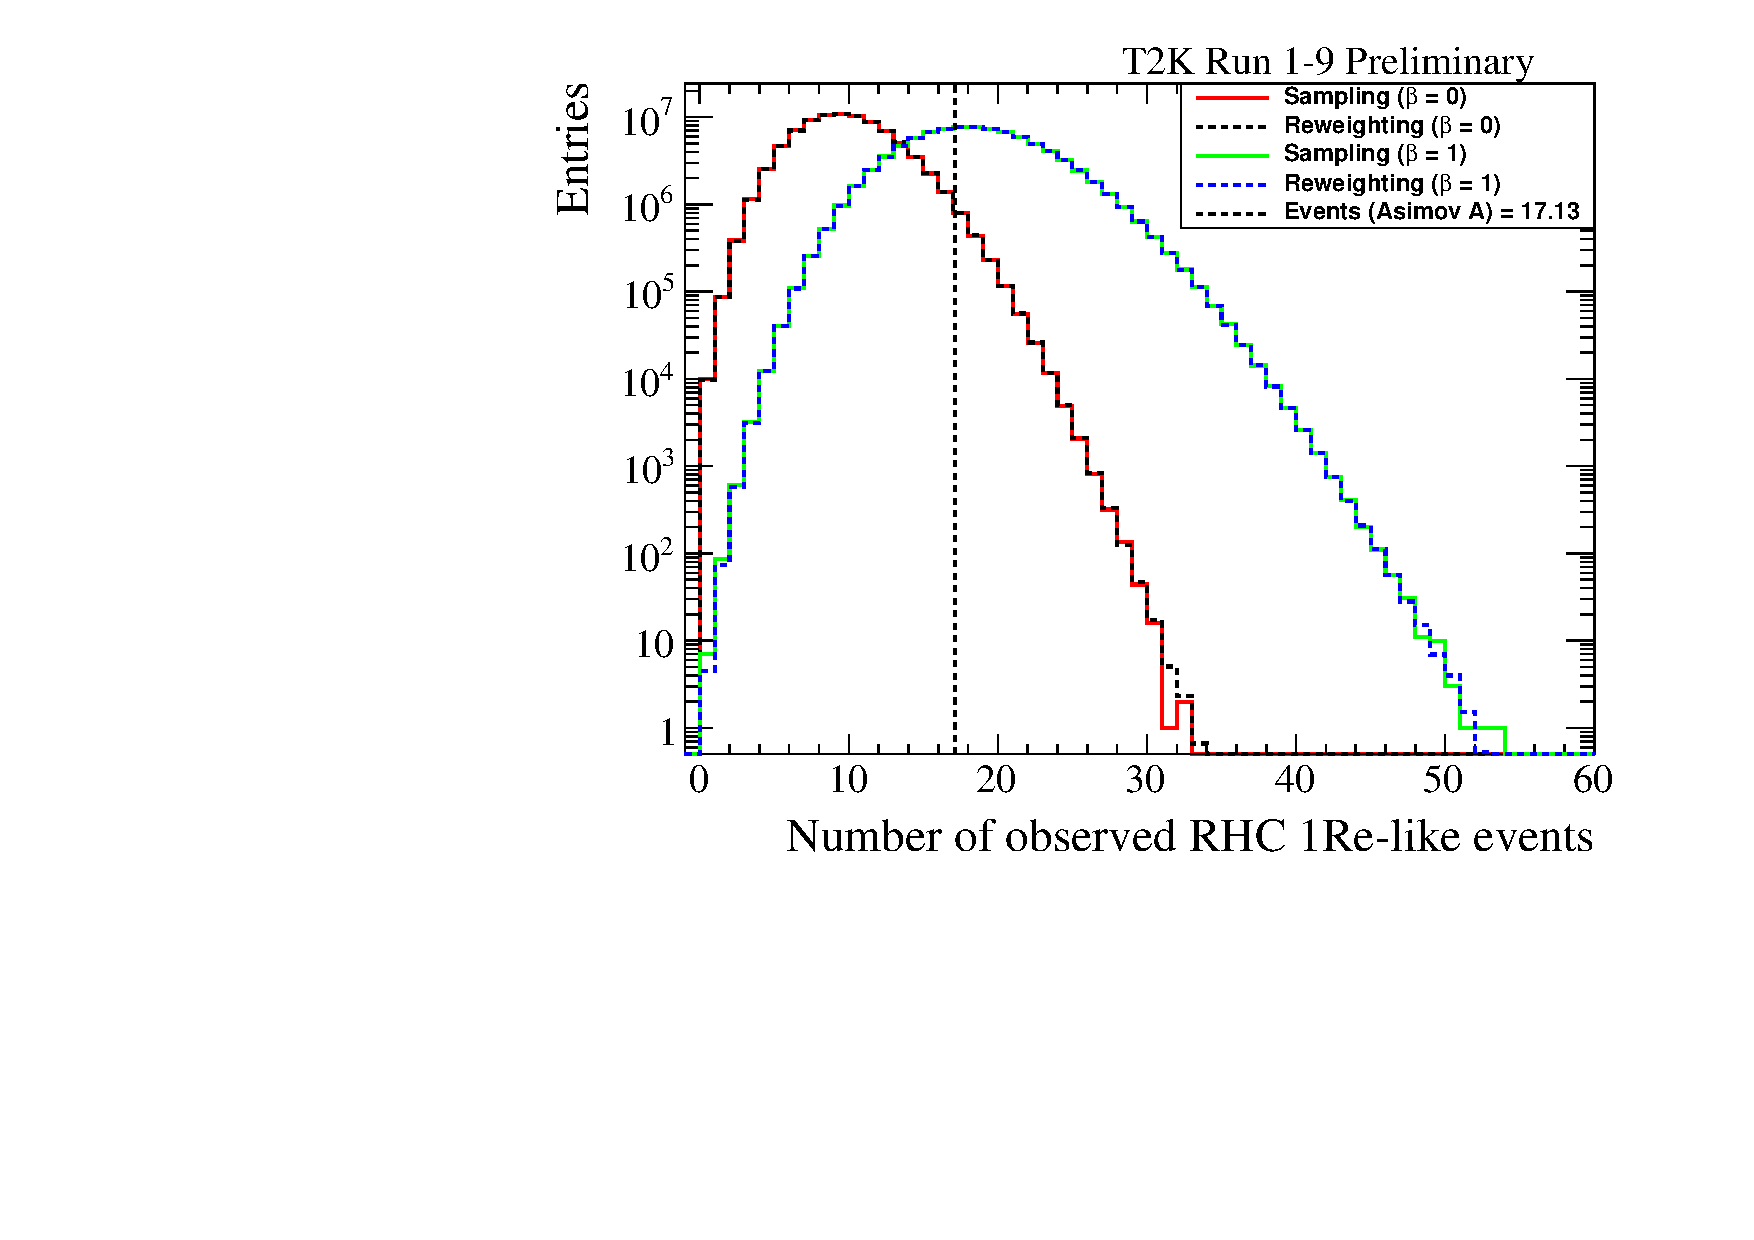
\includegraphics[scale=0.65]{studies/sampling_vs_reweighting/test_sampling_vs_reweighting_rate-only_3500k_Nevents_logscale}
	\caption{Comparison of rate-only test statistic distributions for toy experiments generated by MC sampling and re-weighting. The distribution of the total number of events in the antineutrino mode single-ring e-like sample for both the $\beta = 0$ and $\beta = 1$ hypotheses are produced using full Run 1-9 statistics. The dashed line corresponds to the total number of events given by the Asimov A data set.}
	\label{fig:sensitivity_rate-only_Run1-9d_sampling_test}
\end{figure}

\begin{figure}
	\centering
	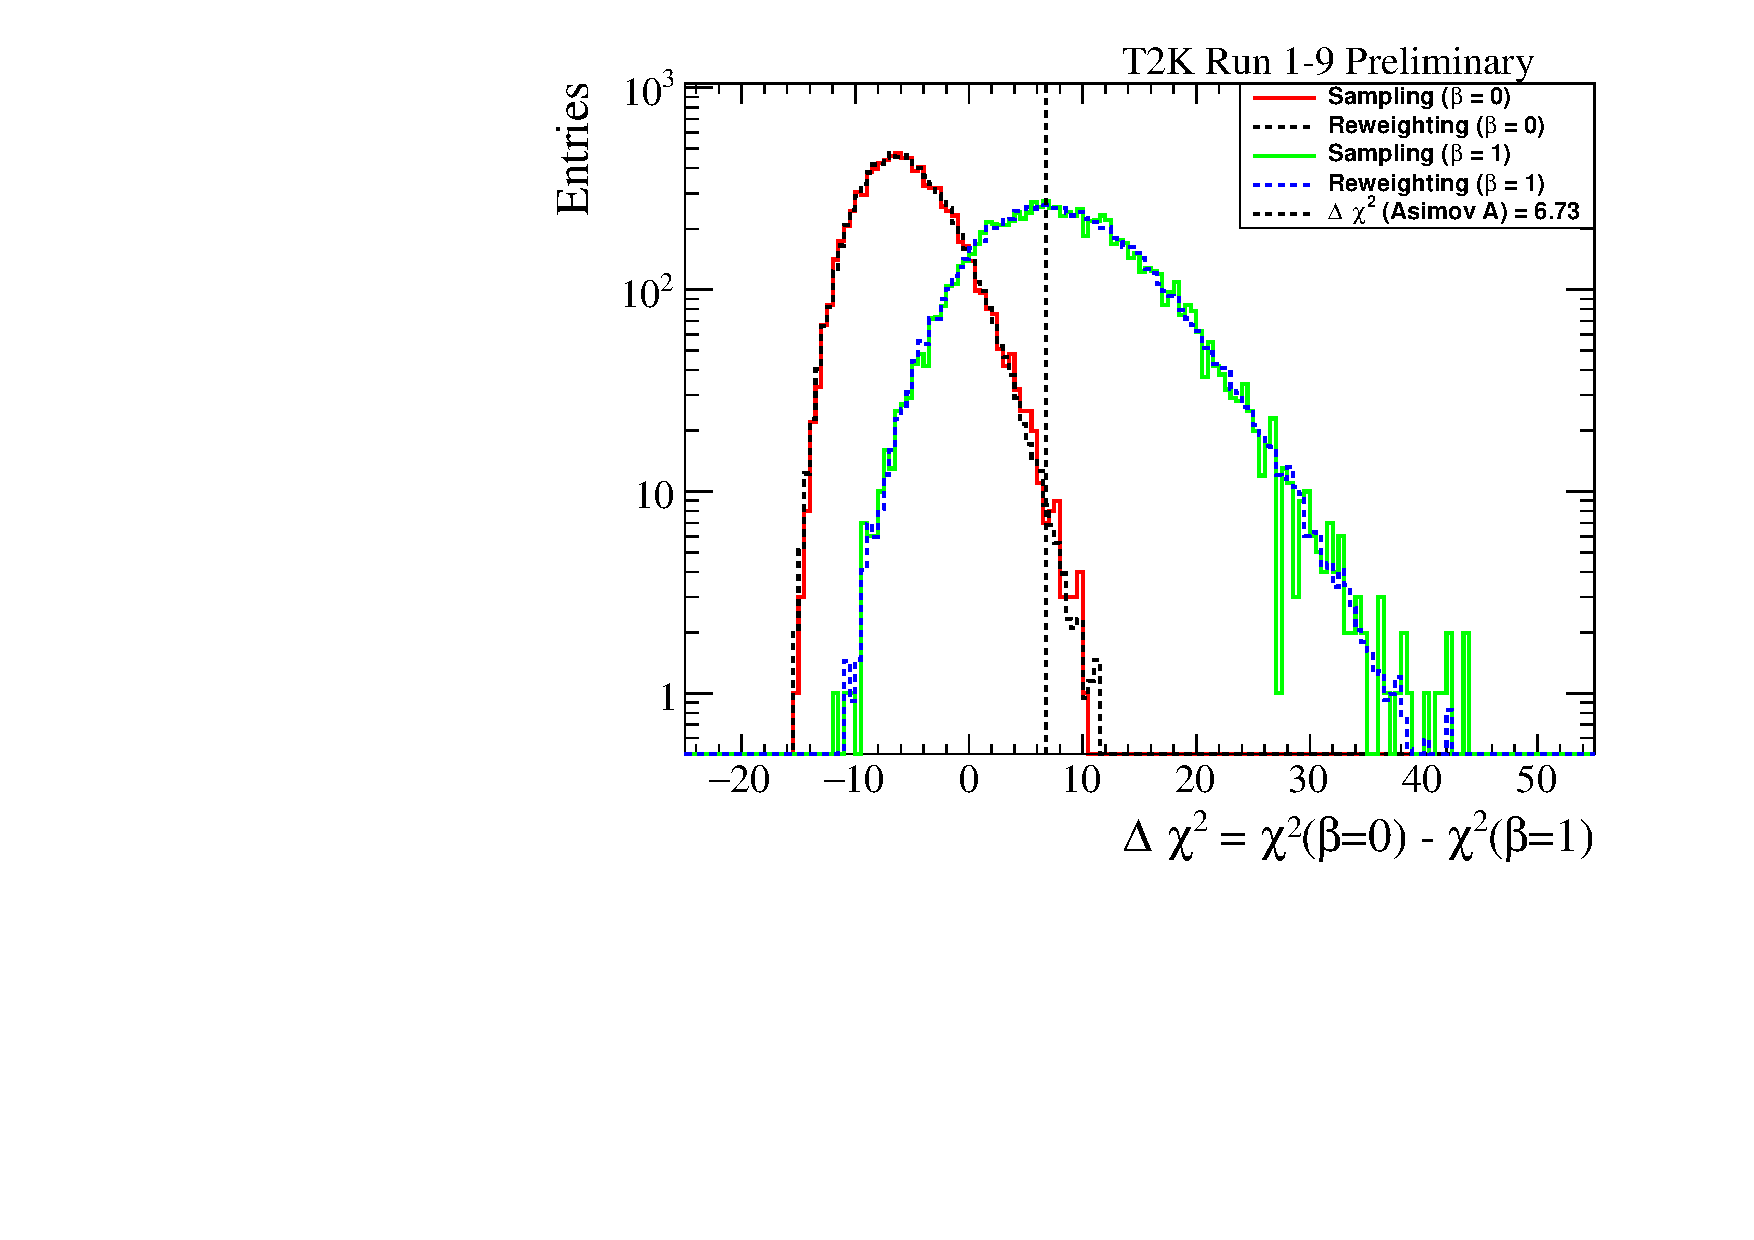
\includegraphics[scale=0.65]{studies/sampling_vs_reweighting/test_sampling_vs_reweighting_rate+shape_3500k_Deltachisq_logscale}
	\caption{Comparison of rate+shape test statistic distributions for toy experiments generated by MC sampling and re-weighting. The distribution of $\Delta \chi^2$ values for both the $\beta = 0$ and $\beta = 1$ hypotheses are produced using full Run 1-9 statistics. The dashed line corresponds to the $\Delta \chi^2$ value given by the Asimov A data set.}
	\label{fig:sensitivity_rate+shape_Run1-9d_sampling_test}
\end{figure}

\begin{table}[H]
\centering
\begin{tabular}{|c|c|c|c|c|}
	\hline
	Analysis                    & Fake data $\beta$   & Toy Gen. Method         & p-value              & $\sigma$               \\
	\hline
	
	
	\multirow{4}{*}{rate-only}  & \multirow{ 2}{*}{0} & MC sampling             & $0.010 \pm 0.001$    & $2.56 \pm 0.04$          \\
	\cline{3-5}
	                            &                     & re-weighting            & $0.01028 \pm 0.00005$& $2.566 \pm 0.002$        \\
	%\cline{3-5}                
	%                           &                     & re-weighting (accepted) & $0.011 \pm 0.001$    & $2.53^{+0.04}_{-0.03}$   \\
	\cline{2-5}
	                            & \multirow{ 2}{*}{1} & MC sampling             & $0.465 \pm 0.005$    & $0.730 \pm 0.009$        \\
	\cline{3-5}
	                            &                     & re-weighting            & $0.4645 \pm 0.0003$  & $0.7315 \pm 0.0004$      \\
	%\cline{3-5}
	%                           &                     & re-weighting (accepted) & $0.482 \pm 0.005$    & $0.703 \pm 0.008$        \\
	\hline
	
	
	\multirow{4}{*}{rate+shape} & \multirow{ 2}{*}{0} & MC sampling             & $0.0040 \pm 0.0007$  & $2.87^{+0.06}_{-0.05}$   \\
	\cline{3-5}
	                            &                     & re-weighting            & $0.0038 \pm 0.0003$  & $2.90 \pm 0.02$          \\
	%\cline{3-5}                
	%                           &                     & re-weighting (accepted) & $0.004 \pm 0.001$    & $2.86^{+0.08}_{-0.07}$   \\
	\cline{2-5}
	                            & \multirow{ 2}{*}{1} & MC sampling             & $0.436 \pm 0.005$    & $0.78 \pm 0.009$         \\
	\cline{3-5}
	                            &                     & re-weighting            & $0.438 \pm 0.002$    & $0.778^{+0.004}_{-0.003}$\\
	%\cline{3-5}
	%                           &                     & re-weighting (accepted) & $0.449 \pm 0.008$    & $0.76 \pm 0.01$          \\
	\hline
	
	
\end{tabular}
\caption{
	Comparison of the p-values obtained using two different toy generation methods, MC sampling and re-weighting.
}
\label{tab:sampling_vs_reweighting_pvals}
\end{table}



} % \colour{red}

\FloatBarrier

	
{\color{red} 

\section{Comparison of Full Run 1-9 vs. Run 1-9c Results}\label{app:compare_R1-9d_R1-9c}

\subsection{Comparison of Expected Sensitivities}\label{app:compare_sensitivity}

Figs \ref{fig:sensitivity_rate-only_Run1-9d_vs_Run1-9c} and \ref{fig:sensitivity_rate+shape_Run1-9d_vs_Run1-9c} show the expected Asimov A sensitivities compared between Run 1-9d and Run 1-9c for the rate-only and rate+shape analyses, respectively. For both analyses, the distributions have broadened and their separation has increased. A comparison of the p-values and test statistics is shown in Tab \ref{tab:sensitivity_comparison_rate_R19d_R17} for the rate-only analysis and for Tab \ref{tab:sensitivity_comparison_shape_R19d_R17} for the rate+shape analysis.

Compared to the Run 1-9c analysis, the Run 1-9d analysis expects a stronger exclusion of the $\beta=0$ hypothesis in both analyses. This is driven by the combination of two factors: 
\begin{enumerate}
	\item The increased statistics further separates the two distributions, as for $\beta=0$ it contains only background events while for $\beta=1$ it contains both signal and background events.
	
	\item The Asimov dataset assumes the $\beta=1$ hypothesis to be true and uses most probable values obtained by the Bayesian analysis on the T2K run 1-4 neutrino mode data \cite{T2KLongPaper}, so its test statistic value is close to the mean value of the $\beta=1$ distribution for each run period.
\end{enumerate}

Both the Run 1-9d and Run 1-9c analyses expect to disfavour the $\beta=1$ hypothesis at an approximately equal level due to the second point above. 


\subsection{Comparison of Data Results} \label{app:compare_data}

Figs \ref{fig:data_rate-only_Run1-9d_vs_Run1-9c} and \ref{fig:data_rate+shape_Run1-9d_vs_Run1-9c} show the observed distributions and test statistics compared between Run 1-9d and Run 1-9c for the rate-only and rate+shape analyses, respectively. A comparison of the p-values and test statistics is shown in Tab \ref{tab:data_comparison_rate_R19d_R17} for the rate-only analysis and for Tab \ref{tab:data_comparison_shape_R19d_R17} for the rate+shape analysis.

For both rate-only and rate+shape analyses, the $\beta=0$ ($\beta=1$) hypothesis is excluded at a greater (lesser) significance in the Run 1-9d analysis than in Run 1-9c. There are two reasons for this change. The first reason is shared by both rate-only and rate+shape analyses - the increased statistics further separates the two distributions (as explained in sec \ref{app:compare_sensitivity}). 

For the rate-only analysis the second reason is that the event rate has increased from $8.01 \frac{\text{events}}{10^{21} \text{POT}}$ in Run 1-9c to $9.18 \frac{\text{events}}{10^{21} \text{POT}}$ in Run 1-9d, shifting the rate-only test statistic closer to the mean value of the $\beta = 1$ distribution and further from the mean of the $\beta = 0$ distribution.

For the rate+shape analysis, the second reason for this change can be seen by comparing Fig \ref{fig:asimova_spectra_Run1-9d_RHC1Re} to Fig \ref{fig:asimova_spectra_RHC1Re}. It  can be seen that of the six newly collected (Run 9d) events in the antineutrino mode single-ring electron-like sample, five events are in the most likely region as predicted by the Asimov A dataset under the assumption of the $\beta = 1$ hypothesis. This is in contrast to the Run 1-9c data, where most of the nine events lay outside this region. This has the effect of changing the data $\Delta \chi^2$ value from the Run 1-9c value of \DeltachisqData\ to the Run 1-9d value of \DeltachisqDataRunOneNineD. This $\Delta \chi^2$ value is now close to the mean of the $\beta=1$ distribution, rather than almost midway between the two distributions, as was the case in Run 1-9c. This change is further demonstrated by the Bayes factor of \BayesFactorDataRunOneNineD\ which corresponds to a substantial preference for the $\beta = 1$ hypothesis over $\beta = 0$, while for the Run 1-9c analysis the Bayes factor was \BayesFactorData\, meaning a poor preference for the $\beta = 0$ hypothesis over $\beta = 1$.

\newpage


\begin{table}
	\centering
	\begin{tabular}{|c|c|c|c|c|c|c|}
		\hline
		\multirow{2}{*}{Run} & \multirow{2}{*}{RHC POT}   & \multirow{2}{*}{$N_{exp}$}    & \multicolumn{2}{|c|}{$\beta=0$} & \multicolumn{2}{|c|}{$\beta=1$} \\
		\cline{4-7}     				
		     		         &                            &   				 	          & p-value        & $\sigma$       & p-value      & $\sigma$         \\
		\hline
		
		
		1-9d                 & \TotalPotNuBarRunOneNine   & \NskOscExpectationNueBarRunOneNineD & \pvalRateOnlyBetaZeroAsimovARunOneNineD & \sigmaRateOnlyBetaZeroAsimovARunOneNineD & \pvalRateOnlyBetaOneAsimovARunOneNineD  & \sigmaRateOnlyBetaOneAsimovARunOneNineD \\
		\hline
		
		
		1-9c                 & \TotalPotNuBarRunOneNineC  & \NskOscExpectationNueBarRunOneNineC & \pvalRateOnlyBetaZeroAsimovA & \sigmaRateOnlyBetaZeroAsimovA & \pvalRateOnlyBetaOneAsimovA & \sigmaRateOnlyBetaOneAsimovA \\
		\hline
		
		
		1-7                  & \TotalPotNuBarRunOneSevenC & 6.008	  & $0.0511 \pm 0.00002$  & $1.9506 \pm 0.0002$		 & $0.5022 \pm 0.00005$   & $0.67103 \pm 0.0008$ \\
		\hline
	\end{tabular}
	\caption{Expected rate-only p-values and the number of events from the full Run 1-9 data set compared to the Run 1-9c and Run 1-7 data set used for previous iterations of this analysis, in Summer 2018 and 2016\cite{OurRun16AntiNueBarAppearanceAnalysis3Flavour}, respectively.}
	\label{tab:sensitivity_comparison_rate_R19d_R17}
\end{table}


\begin{table}
	\centering
	\begin{tabular}{|c|c|c|c|c|c|c|c|}
		\hline
		\multirow{2}{*}{Run} & \multirow{2}{*}{RHC POT} & \multirow{2}{*}{$\Delta \chi^2_{\textrm{exp}}$} & \multicolumn{2}{|c|}{$\beta=0$} & \multicolumn{2}{|c|}{$\beta=1$} & \multirow{2}{*}{$B_{01}$}\\
		\cline{4-7}      				
		                     &   				 	    &                                                 & p-value         & $\sigma$      & p-value         & $\sigma$      &   \\
		\hline
		
		
		1-9d                 & \TotalPotNuBarRunOneNine & \DeltachisqAsimovARunOneNineD                   & \pvalRateShapeBetaZeroAsimovARunOneNineD & \sigmaRateShapeBetaZeroAsimovARunOneNineD & \pvalRateShapeBetaOneAsimovARunOneNineD & \sigmaRateShapeBetaOneAsimovARunOneNineD & \BayesFactorAsimovARunOneNineD \\
		\hline
		
		
		1-9c                 & \TotalPotNuBarRunOneNineC& \DeltachisqAsimovA                              & \pvalRateShapeBetaZeroAsimovA & \sigmaRateShapeBetaZeroAsimovA & \pvalRateShapeBetaOneAsimovA & \sigmaRateShapeBetaOneAsimovA & \BayesFactorAsimovA \\
		\hline
		
		
		1-7                  &\TotalPotNuBarRunOneSevenC& 2.610			                                  & $0.043 \pm 0.002$ & $2.02 \pm 0.02$	  &  $0.444 \pm 0.005$ & $0.765 \pm 0.008$		  & 0.271 \\
		\hline
	\end{tabular}
	\caption{Expected rate+shape p-values, $\Delta \chi^2$ and Bayes factor from the full Run 1-9 data set compared to the Run 1-9c and Run 1-7 data set used for previous iterations of this analysis, in Summer 2018 and 2016\cite{OurRun16AntiNueBarAppearanceAnalysis3Flavour}, respectively.}
	\label{tab:sensitivity_comparison_shape_R19d_R17}
\end{table}

\begin{table}
	\centering
	\begin{tabular}{|c|c|c|c|c|c|c|}
		\hline
		\multirow{2}{*}{Run} & \multirow{2}{*}{RHC POT}   & \multirow{2}{*}{$N_{obs}$}    & \multicolumn{2}{|c|}{$\beta=0$} & \multicolumn{2}{|c|}{$\beta=1$} \\
		\cline{4-7}     				
		     		         &                            &   				 	          & p-value        & $\sigma$       & p-value      & $\sigma$         \\
		\hline
		
		
		1-9d                 & \TotalPotNuBarRunOneNine   & \NskObservedNueBarRunOneNineD & \pvalRateOnlyBetaZeroDataRunOneNineD & \sigmaRateOnlyBetaZeroDataRunOneNineD & \pvalRateOnlyBetaOneDataRunOneNineD  & \sigmaRateOnlyBetaOneDataRunOneNineD \\
		\hline
		
		
		1-9c                 & \TotalPotNuBarRunOneNineC  & \NskObservedNueBarRunOneNineC & \pvalRateOnlyBetaZeroData & \sigmaRateOnlyBetaZeroData & \pvalRateOnlyBetaOneData & \sigmaRateOnlyBetaOneData \\
		\hline
		
		
		1-7                  & \TotalPotNuBarRunOneSevenC & 4			  				  & $0.4100 \pm 0.00005$  & $0.8239 \pm 0.00009$			& $0.2155 \pm 0.00004$       & $1.2486 \pm 0.0001$ \\
		\hline
	\end{tabular}
	\caption{Observed rate-only p-values and number of events from the full Run 1-9 data set compared to the Run 1-9c and Run 1-7 data set used for previous iterations of this analysis, in Summer 2018 and 2016\cite{OurRun16AntiNueBarAppearanceAnalysis3Flavour}, respectively.}
	\label{tab:data_comparison_rate_R19d_R17}
\end{table}


\begin{table}
	\centering
	\begin{tabular}{|c|c|c|c|c|c|c|c|}
		\hline
		\multirow{2}{*}{Run} & \multirow{2}{*}{RHC POT} & \multirow{2}{*}{$\Delta \chi^2_{\textrm{obs}}$} & \multicolumn{2}{|c|}{$\beta=0$} & \multicolumn{2}{|c|}{$\beta=1$} & \multirow{2}{*}{$B_{01}$}\\
		\cline{4-7}      				
		                     &   				 	    &                                                 & p-value         & $\sigma$      & p-value         & $\sigma$      &   \\
		\hline
		
		
		1-9d                 & \TotalPotNuBarRunOneNine & \DeltachisqDataRunOneNineD                      & \pvalRateShapeBetaZeroDataRunOneNineD & \sigmaRateShapeBetaZeroDataRunOneNineD & \pvalRateShapeBetaOneDataRunOneNineD & \sigmaRateShapeBetaOneDataRunOneNineD & \BayesFactorDataRunOneNineD \\
		\hline
		
		
		1-9c                 & \TotalPotNuBarRunOneNineC& \DeltachisqData                                 & \pvalRateShapeBetaZeroData & \sigmaRateShapeBetaZeroData & \pvalRateShapeBetaOneData & \sigmaRateShapeBetaOneData & \BayesFactorData \\
		\hline
		
		
		1-7                  &\TotalPotNuBarRunOneSevenC& -1.930			                              & $0.3742 \pm 0.0048$			& $0.888 \pm 0.009$		    & $0.099 \pm 0.003$		      & $1.65 \pm 0.01$		  & 2.62 \\
		\hline
	\end{tabular}
	\caption{Observed rate+shape p-values, $\Delta \chi^2$ and Bayes factor from the full Run 1-9 data set compared to the Run 1-9c and Run 1-7 data set used for previous iterations of this analysis, in Summer 2018 and 2016\cite{OurRun16AntiNueBarAppearanceAnalysis3Flavour}, respectively.}
	\label{tab:data_comparison_shape_R19d_R17}
\end{table}


\begin{figure}
	\centering
	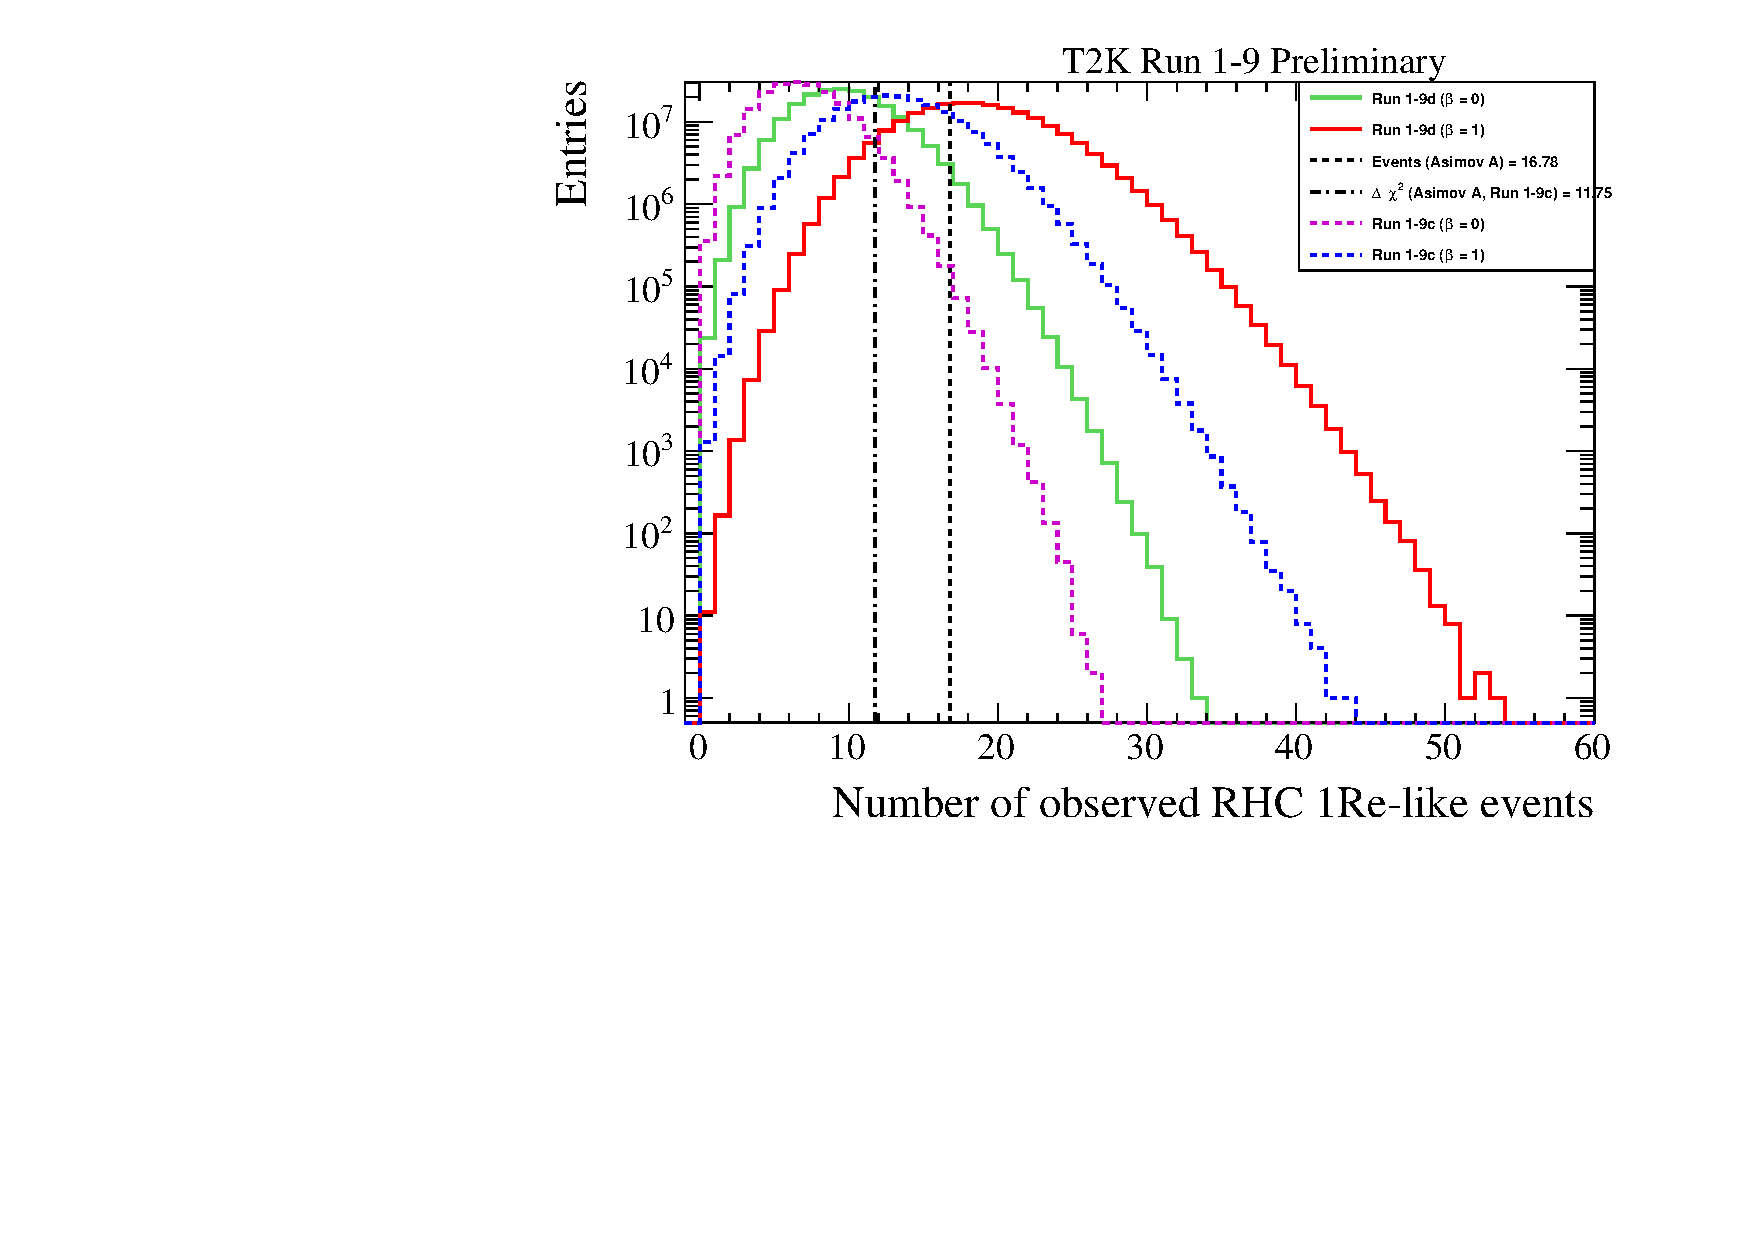
\includegraphics[scale=0.65]{sensitivity/compare_R1-9d_vs_R1-9c/nuebarapp_graphs_nmargtoys=200k_nexp=20k_rate-only_MCsampling_R19d_vs_R19c_comparison_nevents_log}
	\caption{Comparison between the expected Run 1-9d and Run 1-9c distributions of the total number of events in the antineutrino mode single-ring e-like sample. The distributions were produced with \NToysFakeDataRateOnly\ toy experiments for both the $\beta = 0$ and $\beta = 1$ hypotheses using the method outlined in section \ref{sec:method_rate-only} and the Asimov A spectra to calculate the 4-sample likelihood.}
	\label{fig:sensitivity_rate-only_Run1-9d_vs_Run1-9c}
\end{figure}

\begin{figure}
	\centering
	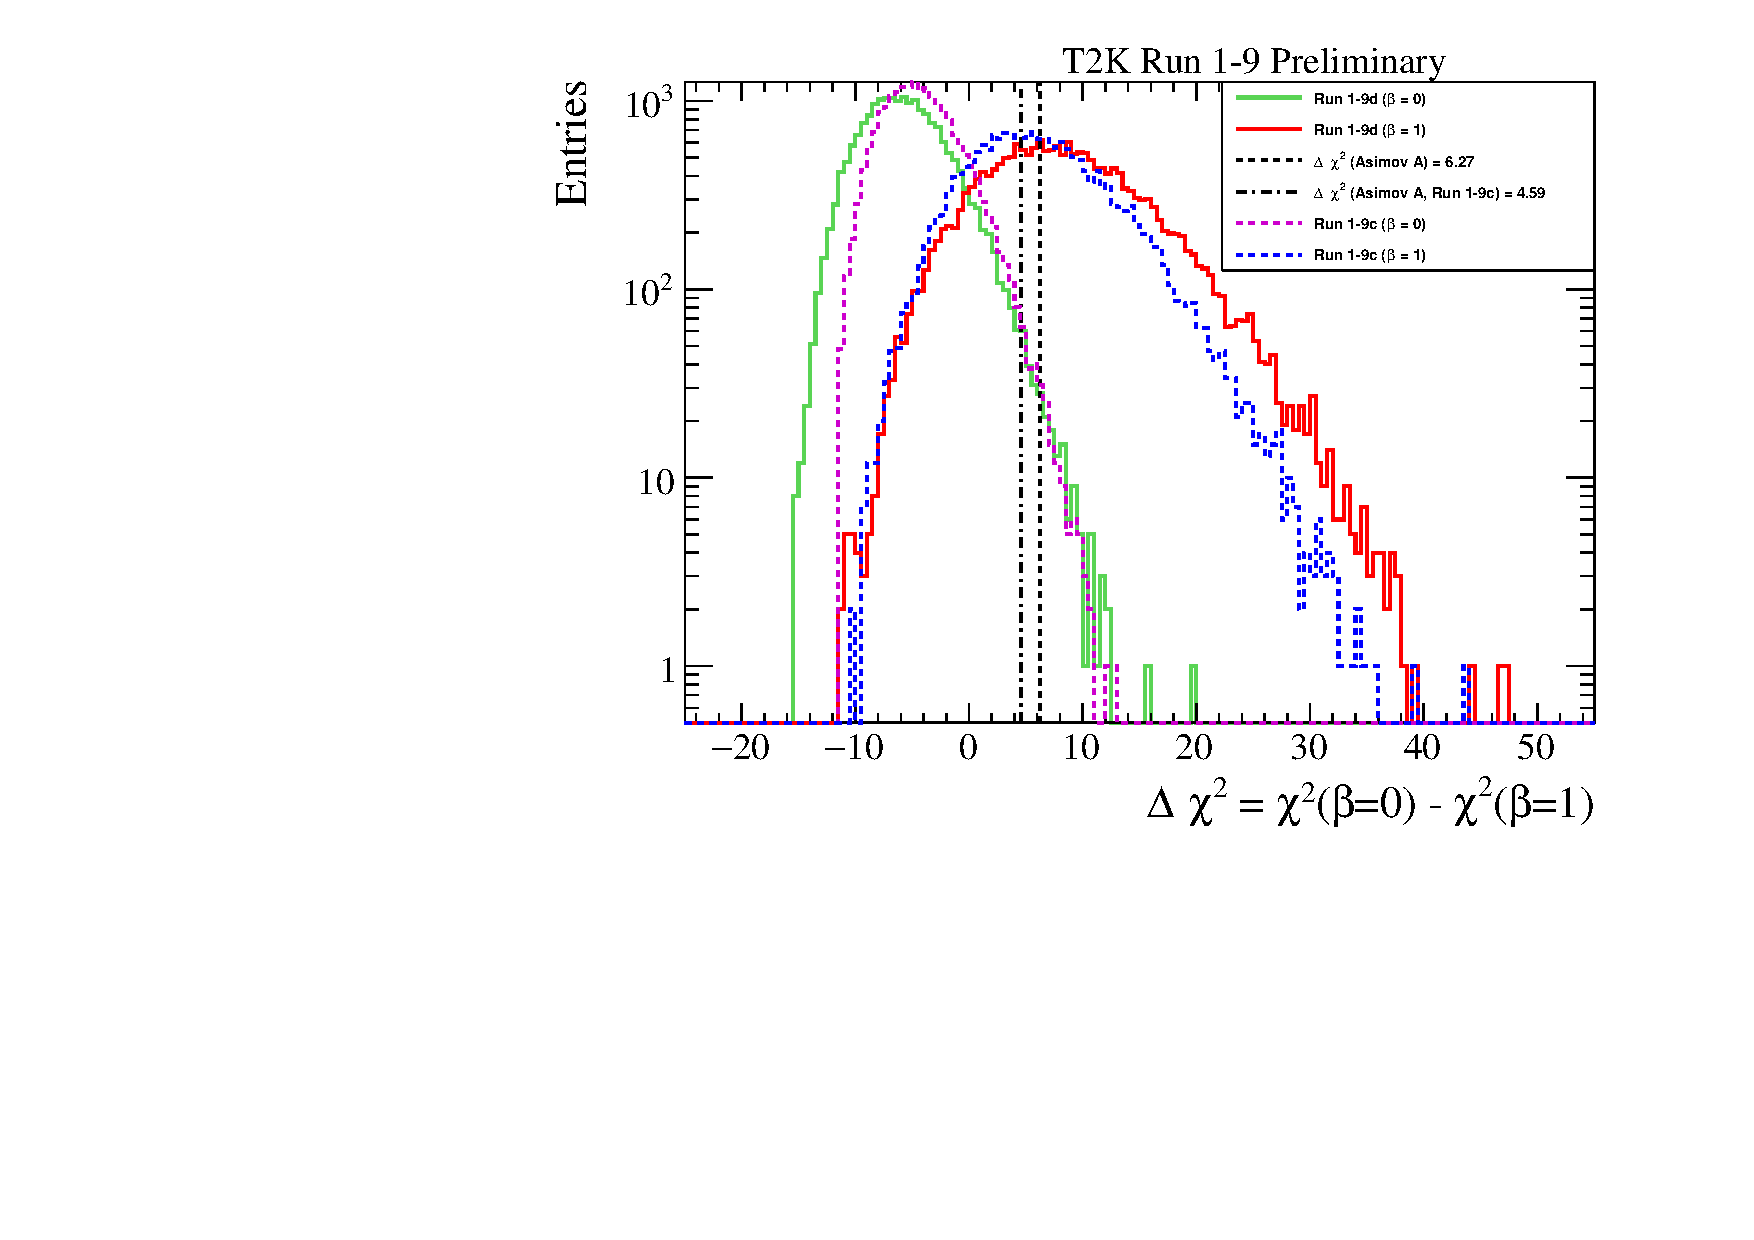
\includegraphics[scale=0.65]{sensitivity/compare_R1-9d_vs_R1-9c/nuebarapp_graphs_nmargtoys=200k_nexp=20k_rate+shape_R19d_vs_R19c_comparison_Deltachisq_log}
	\caption{Comparison between the expected Run 1-9d and Run 1-9c distributions of Asimov-constrained $\Delta \chi^2$ values. The distributions were produced with \NToysFakeDataRatePlusShape\ toy experiments for both the $\beta = 0$ and $\beta = 1$ hypotheses using the method outlined in section \ref{sec:method_rate+shape} with the Asimov A spectra to calculate the 4-sample likelihood.}
	\label{fig:sensitivity_rate+shape_Run1-9d_vs_Run1-9c}
\end{figure}


\begin{figure}
	\centering
	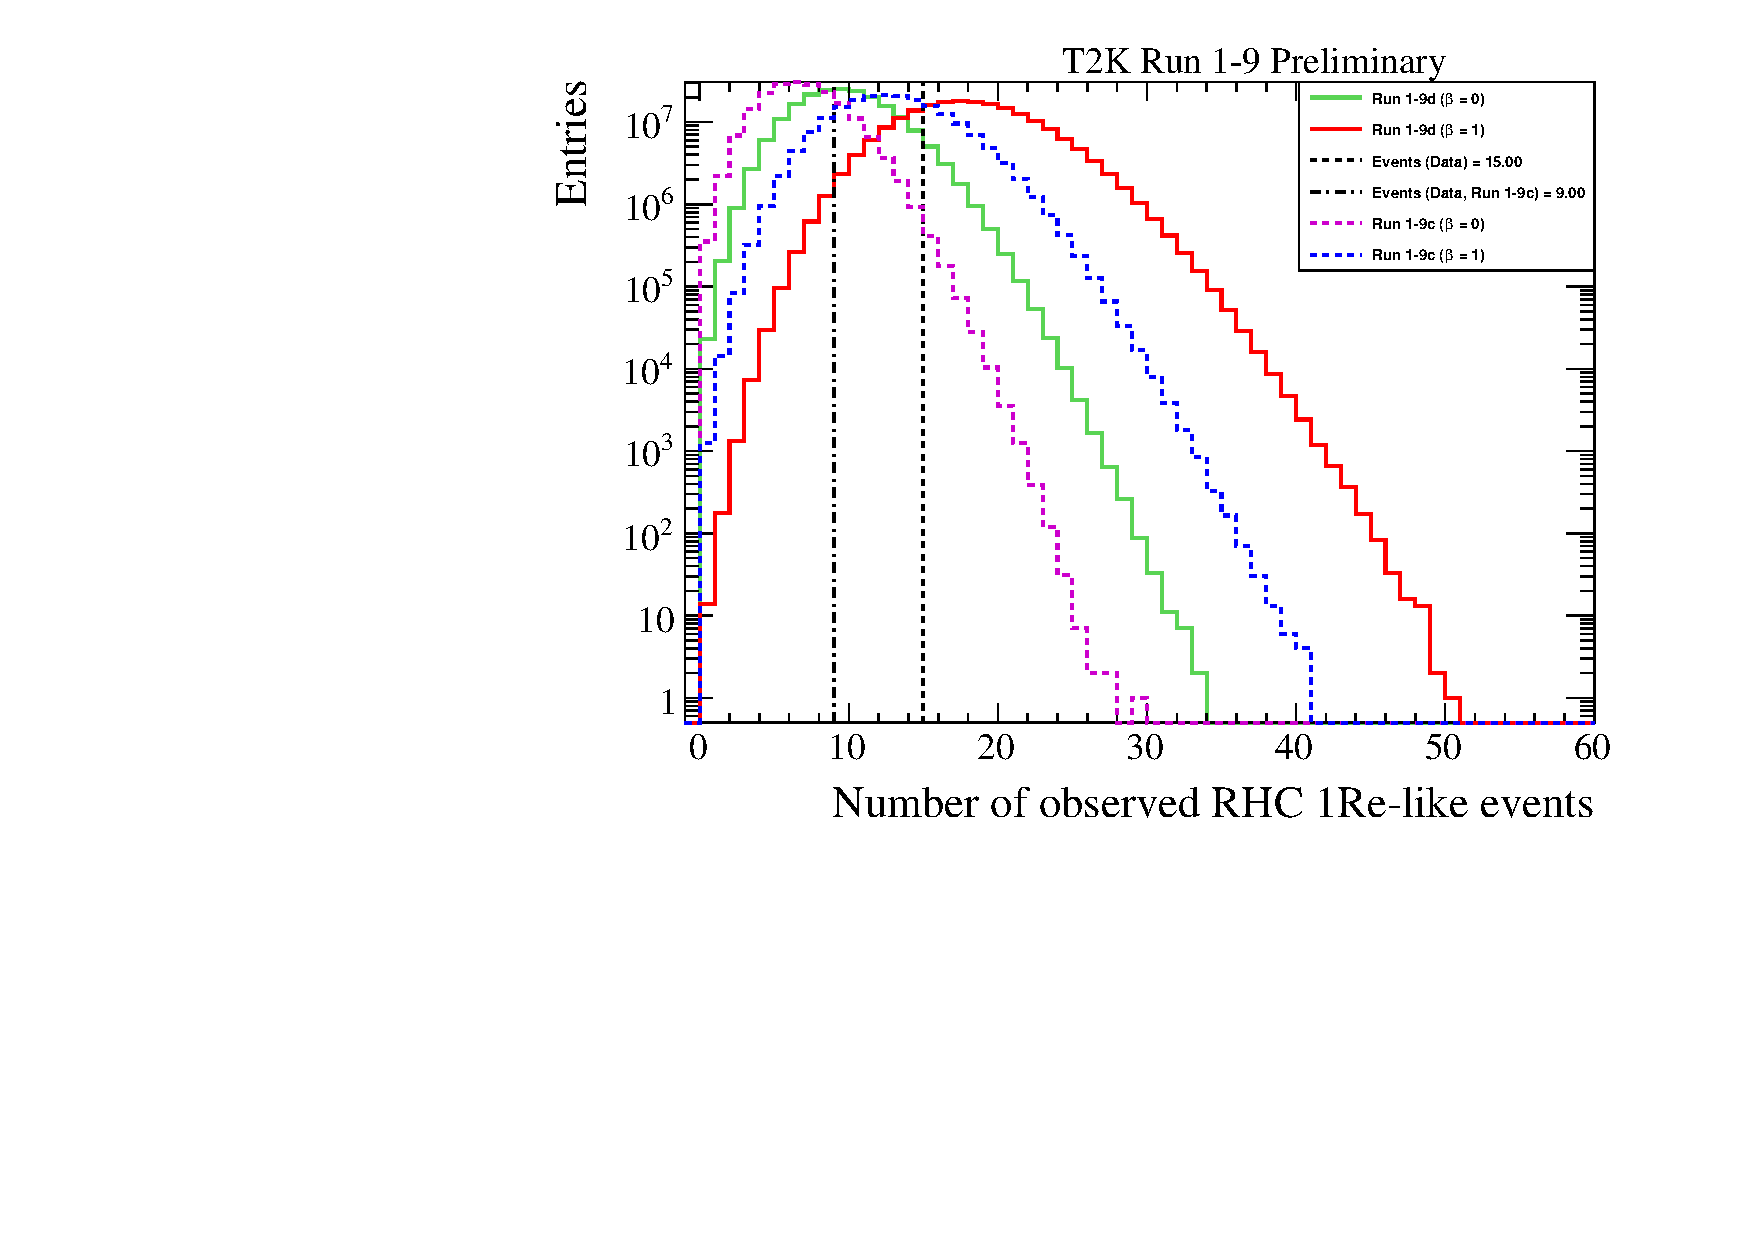
\includegraphics[scale=0.65]{data/compare_R1-9d_vs_R1-9c/nuebarapp_graphs_nmargtoys=200k_nexp=20k_rate-only_Run1-9d_vs_Run1-9c_comparison_nevents_log}
	\caption{Comparison between the observed Run 1-9d and Run 1-9c distributions of the total number of events in the antineutrino mode single-ring e-like sample. The distributions were produced with \NToysFakeDataRateOnly\ toy experiments for both the $\beta = 0$ and $\beta = 1$ hypotheses using the method outlined in section \ref{sec:method_rate-only} and the data spectra to calculate the 4-sample likelihood.}
	\label{fig:data_rate-only_Run1-9d_vs_Run1-9c}
\end{figure}

\begin{figure}
	\centering
	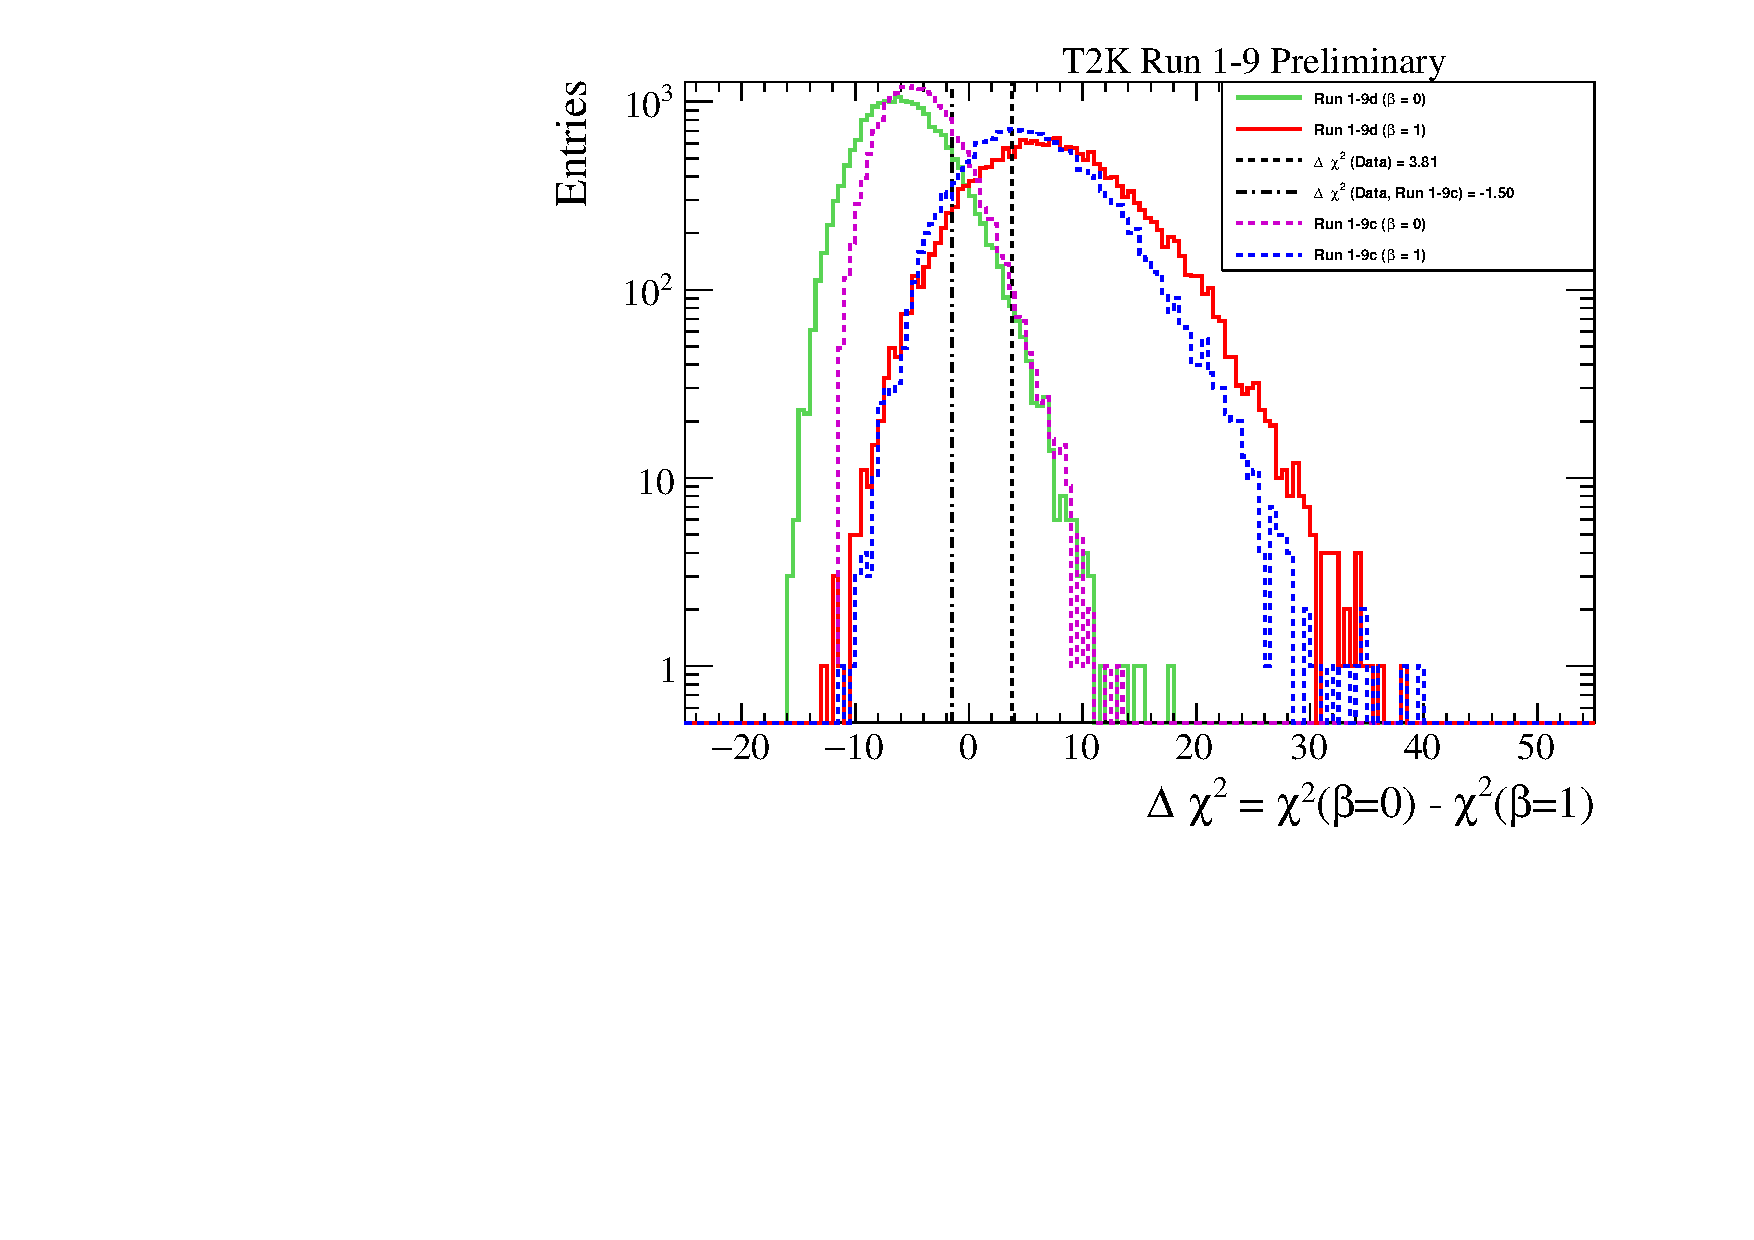
\includegraphics[scale=0.65]{data/compare_R1-9d_vs_R1-9c/nuebarapp_graphs_nmargtoys=200k_nexp=20k_rate+shape_Run1-9d_vs_Run1-9c_comparison_Deltachisq_log}
	\caption{Comparison between the observed Run 1-9d and Run 1-9c distributions of data-constrained $\Delta \chi^2$ values. The distributions were produced with \NToysFakeDataRatePlusShape\ toy experiments for both the $\beta = 0$ and $\beta = 1$ hypotheses using the method outlined in section \ref{sec:method_rate+shape} with the data spectra to calculate the 4-sample likelihood.}
	\label{fig:data_rate+shape_Run1-9d_vs_Run1-9c}
\end{figure}

} % \colour{red}

\FloatBarrier


	\FloatBarrier

{\color{red} 

\section{Comparison Between VALOR and P-theta Results using Full Run 1-9 Statistics} \label{app:compare_valor_ptheta}

To validate the results of this analysis, they are compared to the results obtained by the P-theta group. The P-theta analysis \cite{PthetaR19cNuebarAppearance} uses electron-like spectra binned in $(p, \theta)$ variables, while the VALOR analysis uses $(E_{\text{rec}}, \theta)$. The use of different binning variables will cause the calculation of the control sample likelihood weights (in both rate-only and rate+shape analyses) and marginal likelihood to be different between VALOR and P-theta. Therefore the p-values in the P-theta tech note (see ref \cite{PthetaR19cNuebarAppearance}) are not directly comparable to the p-values in this document. Instead the P-theta group has duplicated their rate+shape analyses using $(E_{\text{rec}}, \theta)$ binning to produce the p-values which are considered in this section.


\subsection{Comparison of Expected Sensitivities}\label{app:compare_sensitivity_valor_ptheta}

The P-theta analysis was completed before the Asimov A true value of $\sin^{2} 2 \theta_{13}$ was updated to 0.0830, so used the previous value of 0.0856. In order to have directly comparable p-values, the VALOR p-values shown in this section were produced using the same value of $\sin^{2} 2 \theta_{13}$ as used in the P-theta analysis, so are not the same p-values shown in section \ref{sec:run1-9d_sensitivity}.

For the rate-only analysis, VALOR expects a test statistic of 17.13 events, while P-theta expects 17.15 events. For the rate+shape analysis, VALOR expects a test statistic of $\Delta \chi^2 = 6.73$, while P-theta expects $\Delta \chi^2 = 6.69$. Figs \ref{fig:sensitivity_rate-only_valor_vs_ptheta} and \ref{fig:sensitivity_rate+shape_valor_vs_ptheta} show the expected rate-only and rate+shape test statistic distributions. As Tab \ref{tab:compare_pvals_sensitivity_valor_ptheta} shows, the p-values produced by VALOR and P-theta are in good agreement.

\begin{table}[H]
\centering
\begin{tabular}{|c|c|c|c|c|}
	\hline
	Analysis                    & Fake data $\beta$   & Group                   & p-value              & $\sigma$                \\
	\hline
	
	
	\multirow{4}{*}{rate-only}  & \multirow{ 2}{*}{0} & VALOR                   & $0.0102 \pm 0.0007$  & $2.57 \pm 0.02$         \\
	\cline{3-5}
	                            &                     & P-theta                 & $0.0109$             & $2.55$                  \\
	\cline{2-5}
	                            & \multirow{ 2}{*}{1} & VALOR                   & $0.465 \pm 0.004$    & $0.73 \pm 0.01$         \\
	\cline{3-5}
	                            &                     & P-theta                 & $0.453$              & $0.75$                  \\
	\hline
	
	
	\multirow{4}{*}{rate+shape} & \multirow{ 2}{*}{0} & VALOR                   & $0.0046 \pm 0.0005$  & $2.83^{+0.04}_{-0.03}$  \\
	\cline{3-5}
	                            &                     & P-theta                 & 0.00369              & 2.90                    \\
	\cline{2-5}
	                            & \multirow{ 2}{*}{1} & VALOR                   & $0.439 \pm 0.004$    & $0.77 \pm 0.01$         \\
	\cline{3-5}
	                            &                     & P-theta                 & 0.429                & 0.79                    \\
	\hline
	
	
\end{tabular}
\caption{
	Comparison of the p-values given by the Asimov A sensitivity studies from the VALOR and P-theta groups.
}
\label{tab:compare_pvals_sensitivity_valor_ptheta}
\end{table}





\subsection{Comparison of Data Results} \label{app:compare_data_valor_ptheta}

For the rate-only analysis the observed test statistic, the event rate in the antineutrino mode single-ring e-like sample (\NskObservedNueBarRunOneNineD\ events) is the same for VALOR and P-theta, as expected. For the rate+shape analysis, differences in the ensemble of marginalisation toys causes slightly different observed $\Delta \chi^2$ values, 3.81 for VALOR and 4.09 for P-theta. Figs \ref{fig:data_rate-only_valor_vs_ptheta} and \ref{fig:data_rate+shape_valor_vs_ptheta} show the observed rate-only and rate+shape test statistic distributions. As Tab \ref{tab:compare_pvals_data_valor_ptheta} shows, the p-values produced by VALOR and P-theta are in good agreement, with the exception of the rate-only $\beta = 1$ p-value. This discrepancy is thought to be due to the fact that for the rate-only analysis, the P-theta group has only used $(p, \theta)$ binning to calculate the control sample likelihood weights (see appendix \ref{app:sampling_vs_reweighting}), and an equivalent rate-only analysis using $(E_{\text{rec}}, \theta)$ binning is not available. This difference is not seen in the rate-only sensitivity study, similarly to the Run 1-9 joint analysis \cite{OurRun19JointAnalysis3Flavour}, where differences in the oscillation parameter confidence intervals produced by VALOR and P-theta are seen in the data fits but not in the sensitivity study.



\begin{table}[H]
\centering
\begin{tabular}{|c|c|c|c|c|}
	\hline
	Analysis                    & Fake data $\beta$   & Group                   & p-value              & $\sigma$                \\
	\hline
	
	
	\multirow{4}{*}{rate-only}  & \multirow{ 2}{*}{0} & VALOR                   & $0.059 \pm 0.002$    & $1.89^{+0.02}_{-0.01}$  \\
	\cline{3-5}
	                            &                     & P-theta                 & 0.0686               & 1.82                    \\
	\cline{2-5}
	                            & \multirow{ 2}{*}{1} & VALOR                   & $0.321 \pm 0.003$    & $0.99 \pm 0.01$         \\
	\cline{3-5}
	                            &                     & P-theta                 & 0.246                & 1.16                    \\
	\hline
	
	
	\multirow{4}{*}{rate+shape} & \multirow{ 2}{*}{0} & VALOR                   & $0.0163 \pm 0.0009$  & $2.40 \pm 0.02$         \\
	\cline{3-5}
	                            &                     & P-theta                 & 0.0155               & 2.42                    \\
	\cline{2-5}
	                            & \multirow{ 2}{*}{1} & VALOR                   & $0.300 \pm 0.004$    & $1.04 \pm 0.01$         \\
	\cline{3-5}
	                            &                     & P-theta                 & 0.300                & 1.04                    \\
	\hline
	
	
\end{tabular}
\caption{
	Comparison of the observed p-values from the VALOR and P-theta groups.
}
\label{tab:compare_pvals_data_valor_ptheta}
\end{table}



\FloatBarrier

\begin{figure}
	\centering
	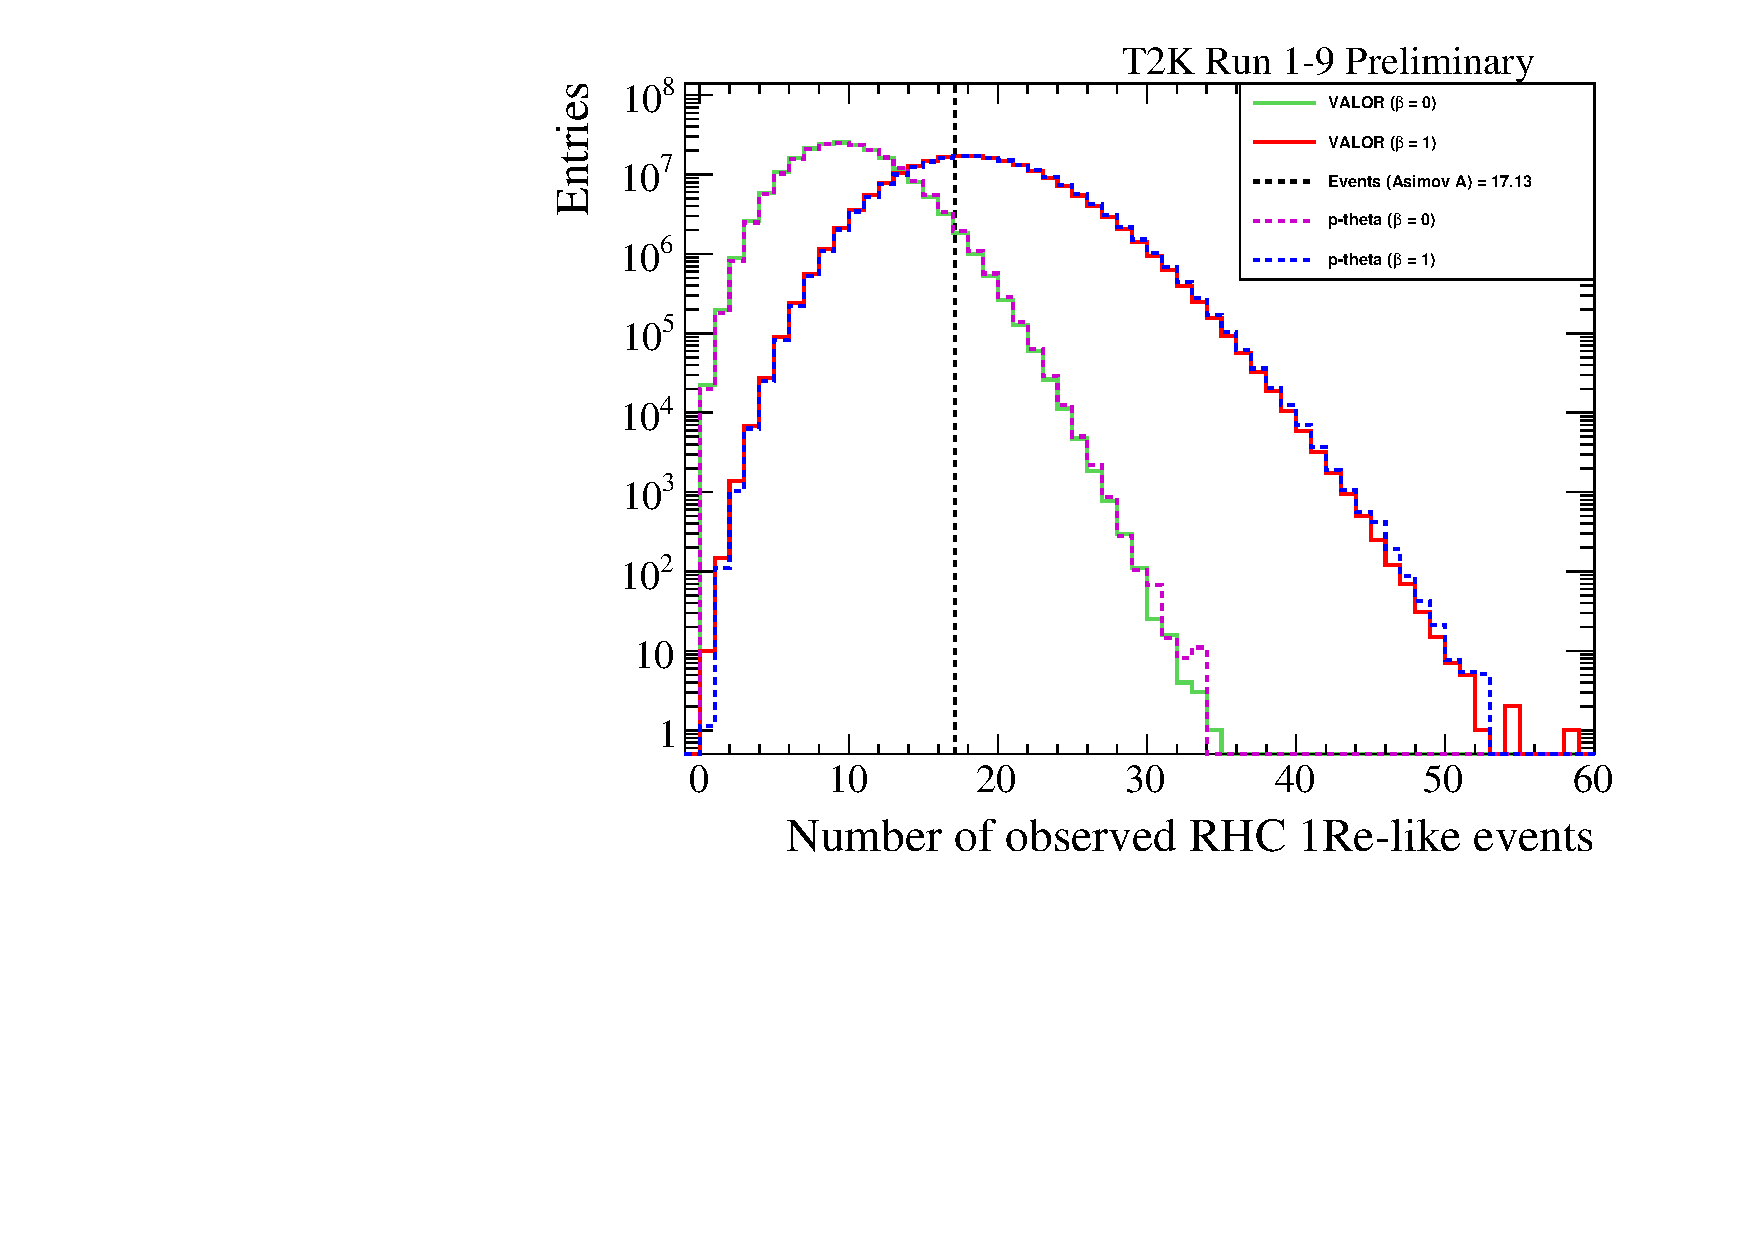
\includegraphics[scale=0.65]{sensitivity/compare_valor_ptheta_R1-9d/nuebarapp_graphs_nmargtoys=200k_nexp=20k_rate-only_MCsampling_VALOR_vs_ptheta_logscale_comparison_nevents}
	
	\caption{Comparison between the expected VALOR and P-theta distributions of the total number of events in the antineutrino mode single-ring e-like sample. The VALOR distributions were produced with \NToysFakeDataRateOnly\ toy experiments using MC sampling (see appendix \ref{app:sampling_vs_reweighting}). The P-theta distributions were produced with 100k toy experiments using re-weighting. Asimov A spectra were used to calculate the 4-sample likelihood.}
	
	\label{fig:sensitivity_rate-only_valor_vs_ptheta}
\end{figure}

\begin{figure}
	\centering
	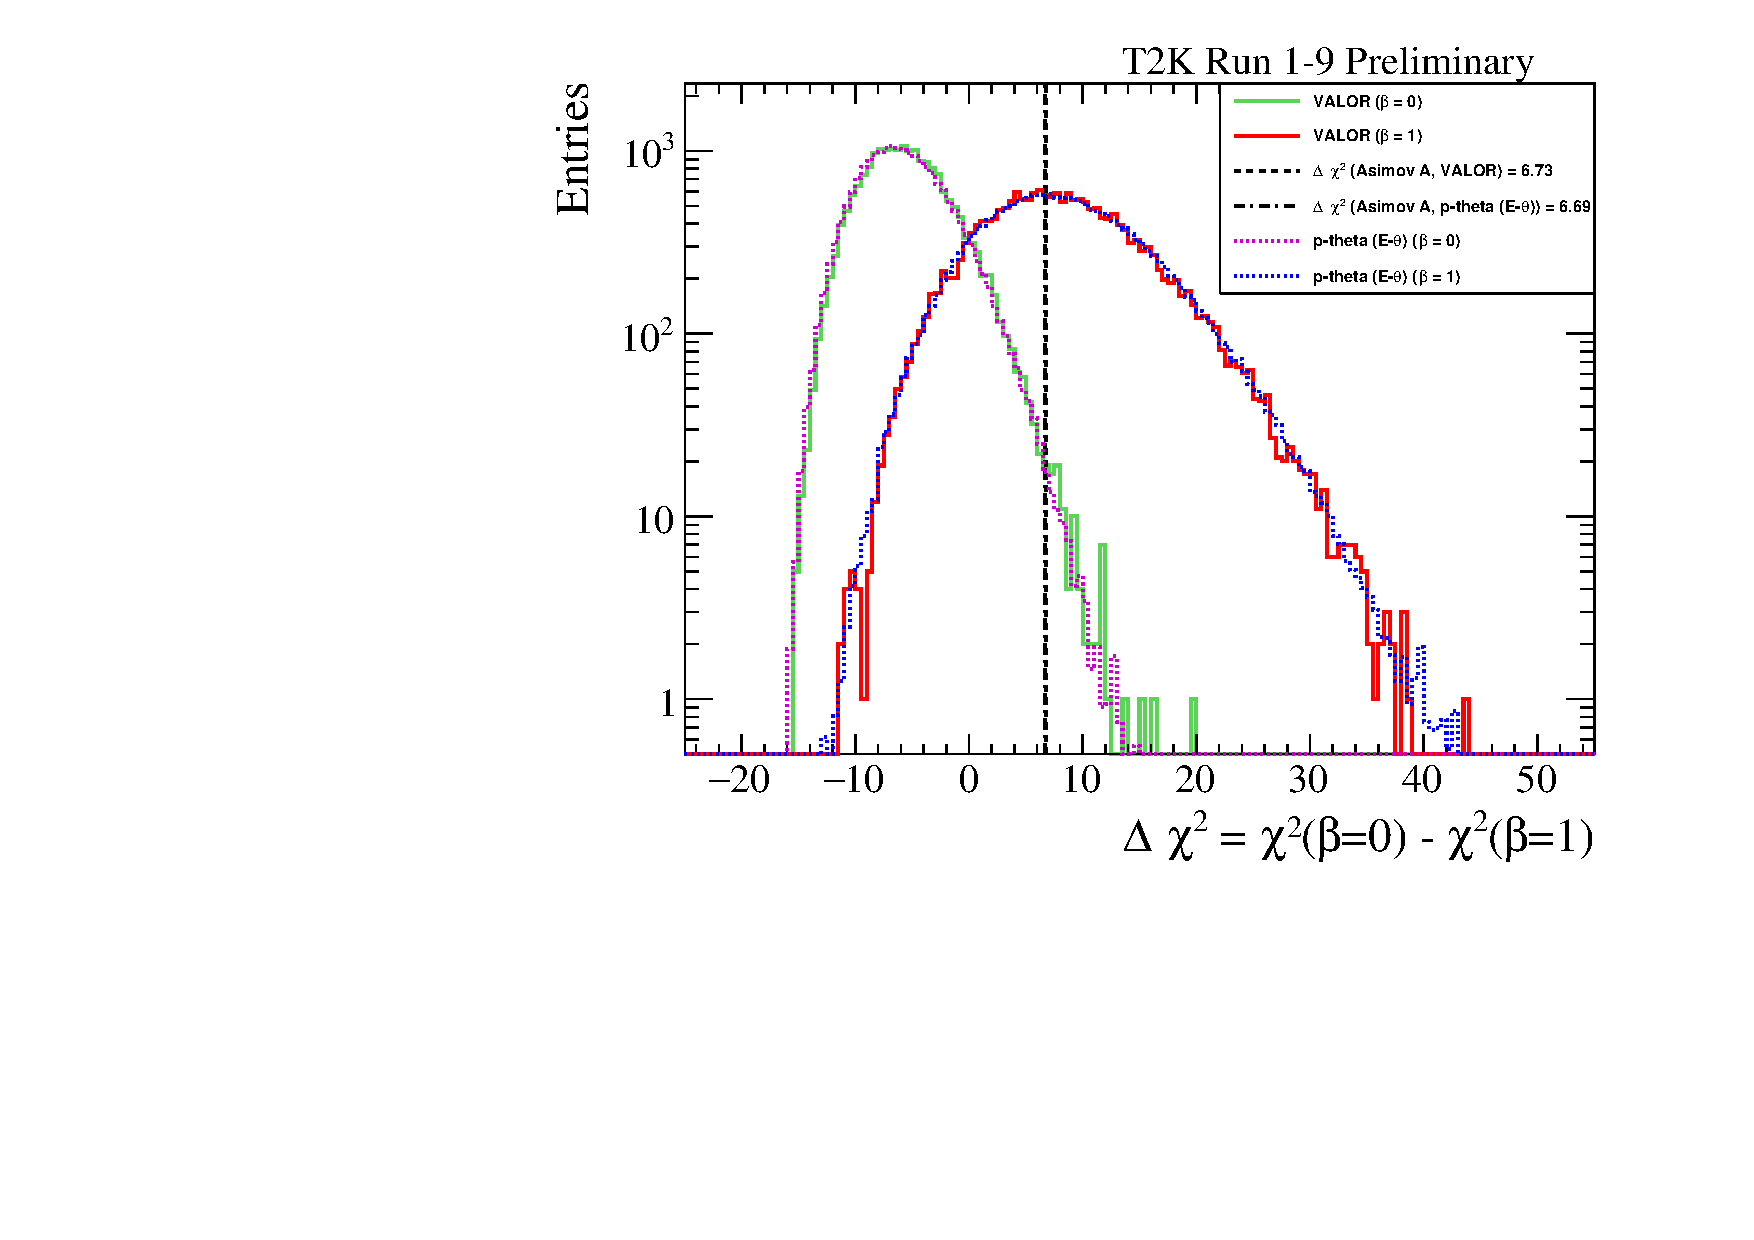
\includegraphics[scale=0.65]{sensitivity/compare_valor_ptheta_R1-9d/nuebarapp_graphs_nmargtoys=200k_nexp=20k_rate+shape_method2_MCsampling_VALOR_vs_ptheta_etheta_logscale_comparison_Deltachisq}
	
	\caption{Comparison between the expected VALOR and P-theta $\Delta \chi^2$ distributions. The VALOR distributions were produced with \NToysFakeDataRateOnly\ toy experiments using MC sampling (see appendix \ref{app:sampling_vs_reweighting}). The P-theta distributions were produced with 2000k toy experiments using re-weighting. Asimov A spectra were used to calculate the 4-sample likelihood.}
	
	\label{fig:sensitivity_rate+shape_valor_vs_ptheta}
\end{figure}



\begin{figure}
	\centering
	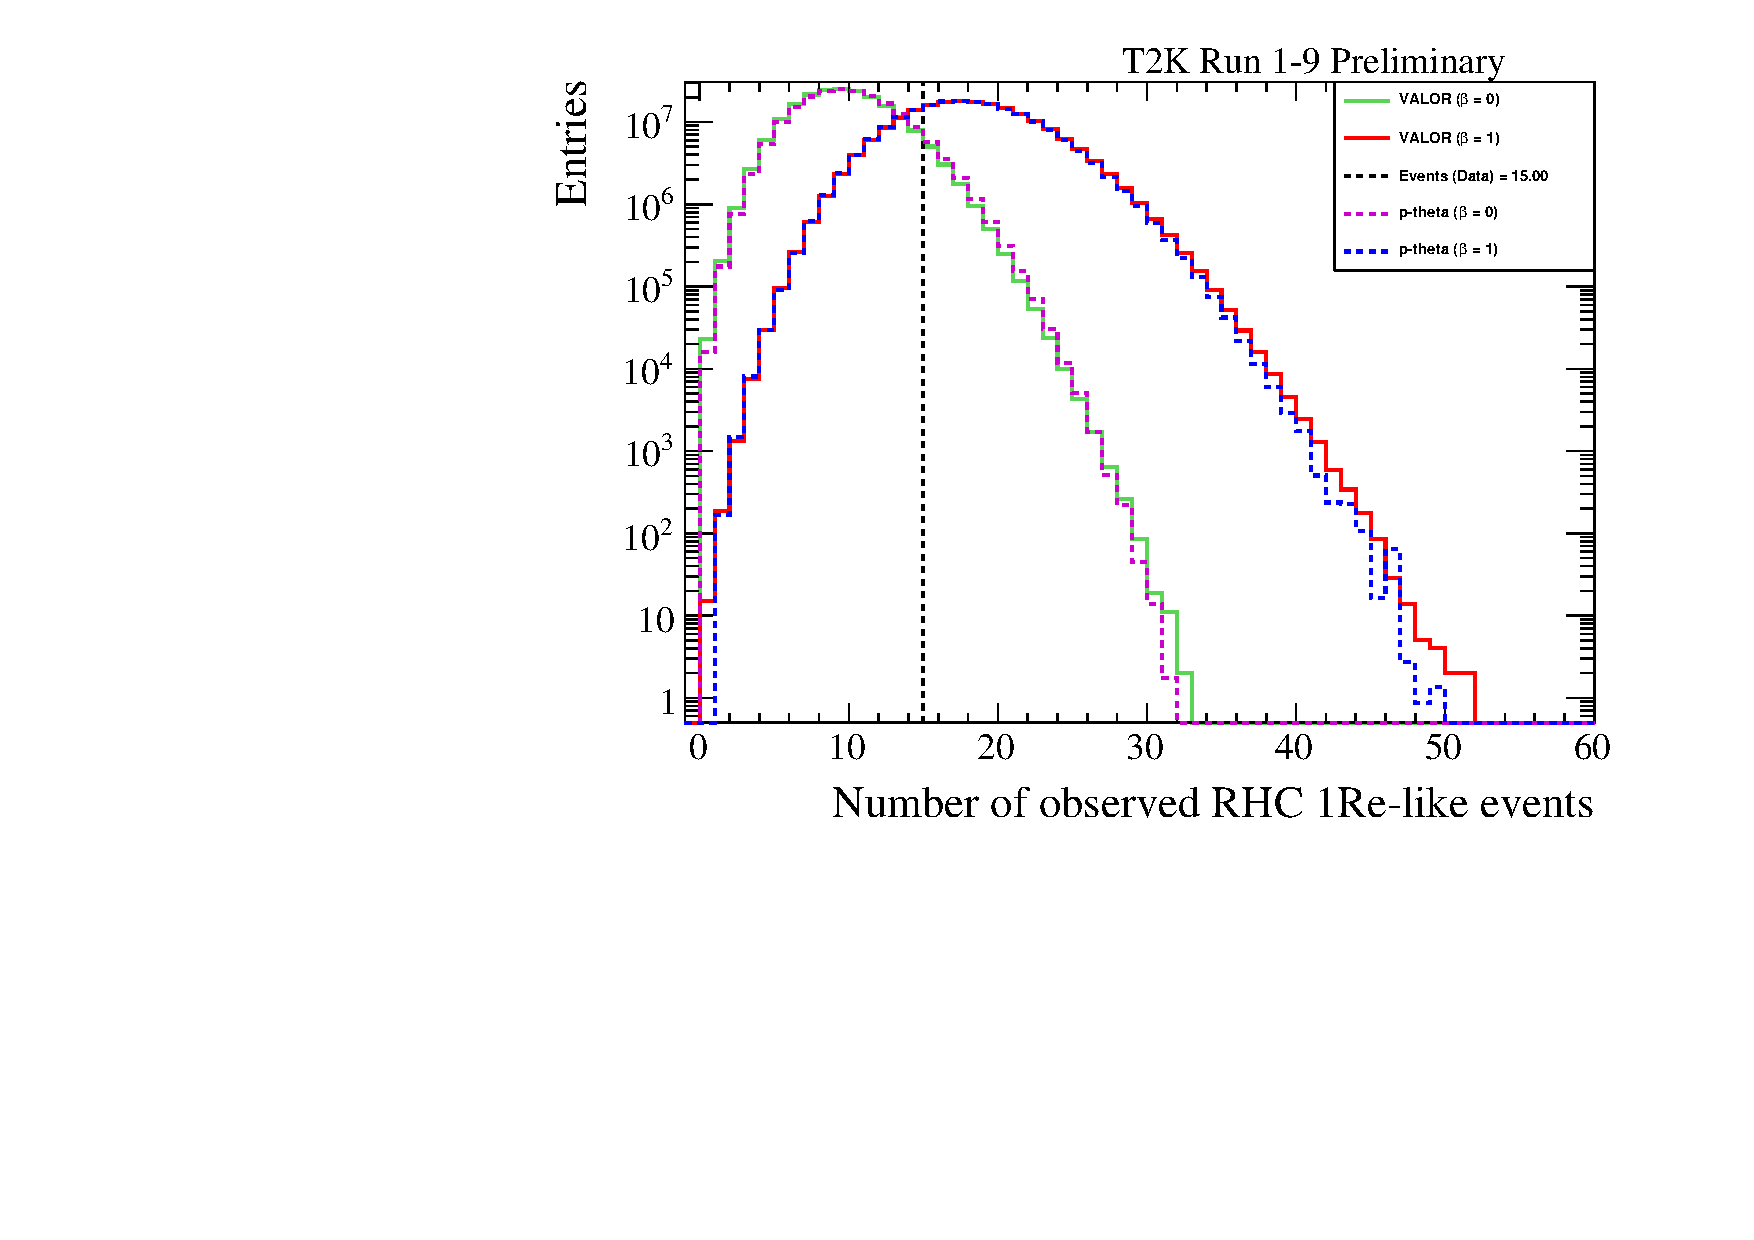
\includegraphics[scale=0.65]{data/compare_valor_ptheta_R1-9d/nuebarapp_graphs_nmargtoys=200k_nexp=20k_data_rate-only_MCsampling_VALOR_vs_ptheta_comparison_nevents_log}
	
	\caption{Comparison between the observed VALOR and P-theta distributions of the total number of events in the antineutrino mode single-ring e-like sample. The VALOR distributions were produced with \NToysFakeDataRateOnly\ toy experiments using MC sampling (see appendix \ref{app:sampling_vs_reweighting}). The P-theta distributions were produced with 100k toy experiments using re-weighting. Observed Run 1-9 spectra were used to calculate the 4-sample likelihood.}
	
	\label{fig:data_rate-only_valor_vs_ptheta}
\end{figure}

\begin{figure}
	\centering
	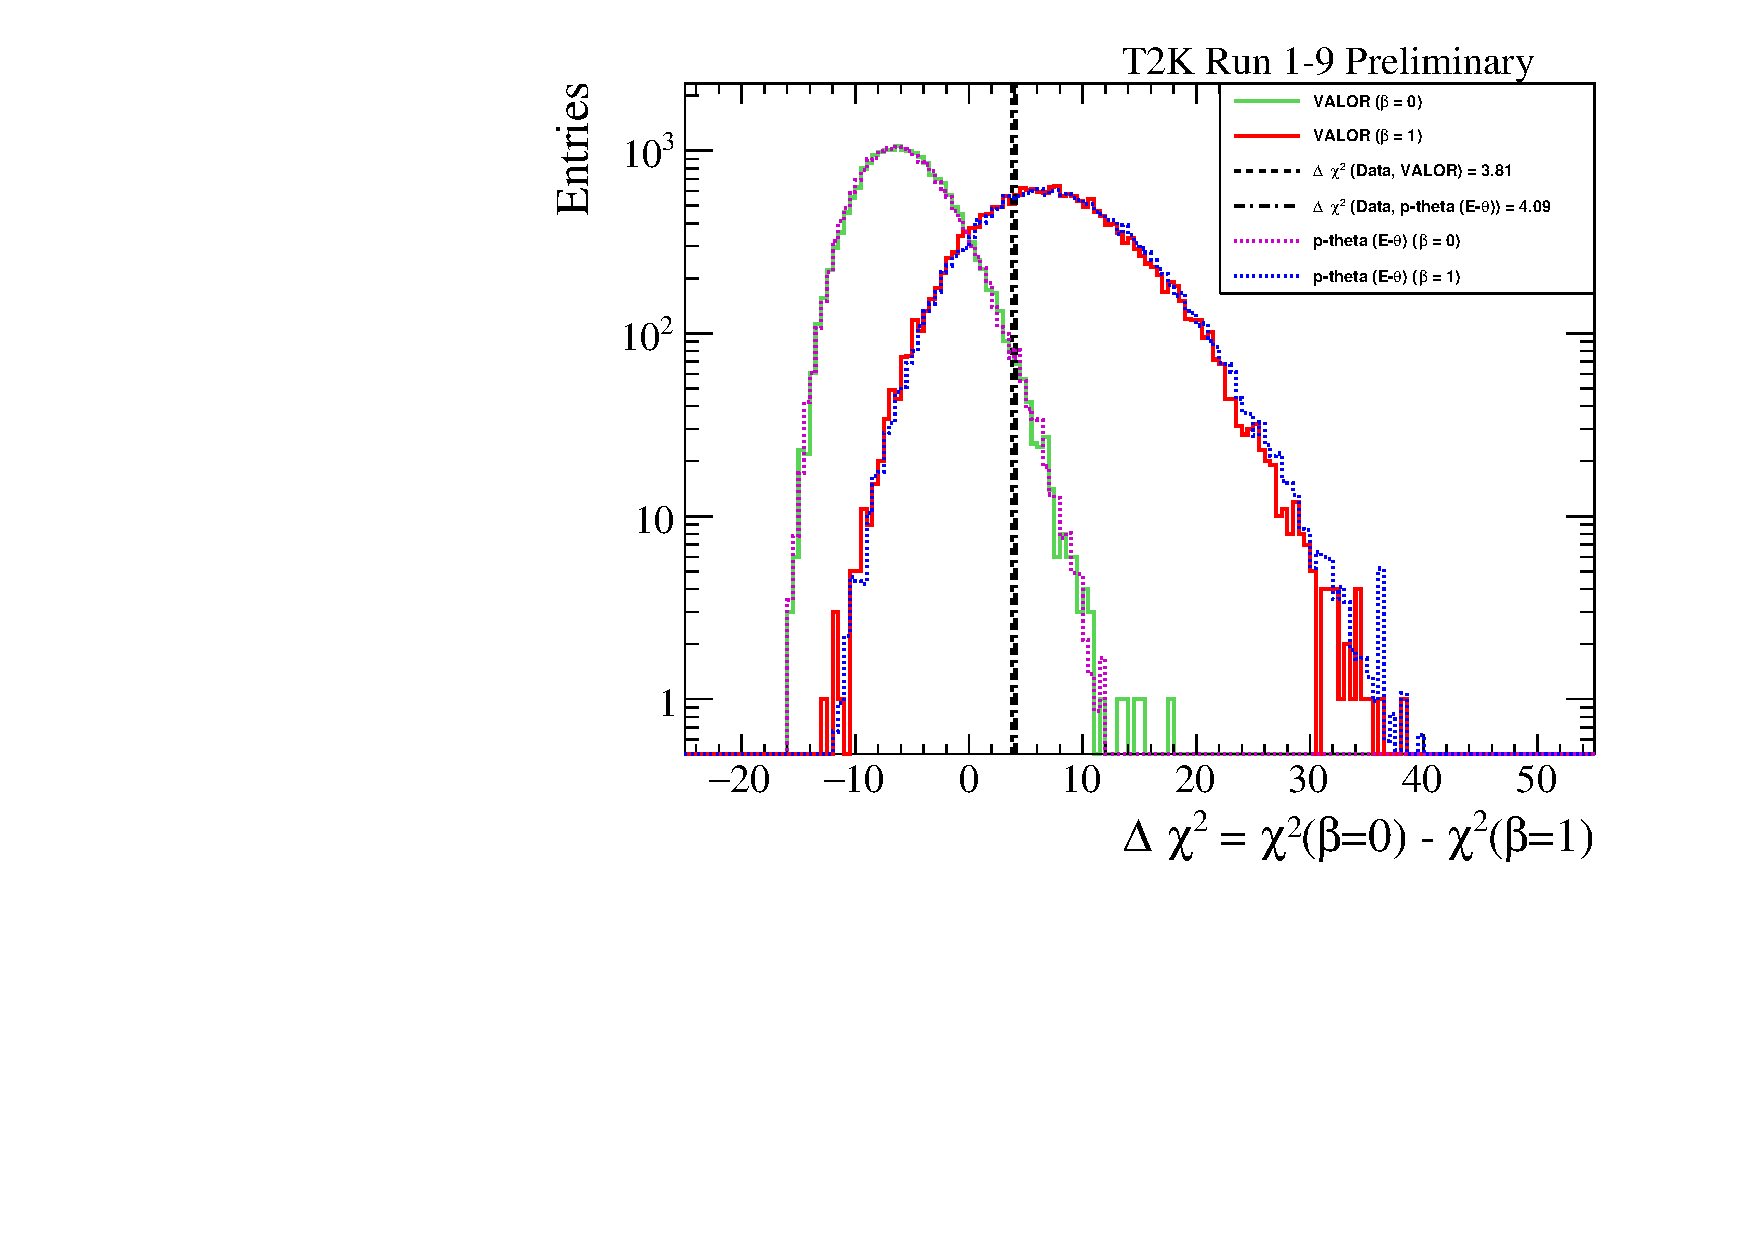
\includegraphics[scale=0.65]{data/compare_valor_ptheta_R1-9d/nuebarapp_graphs_nmargtoys=200k_nexp=20k_data_rate+shape_method2_MCsampling_VALOR_vs_ptheta_etheta_logscale_comparison_Deltachisq}
	
	\caption{Comparison between the observed VALOR and P-theta $\Delta \chi^2$ distributions. The VALOR distributions were produced with \NToysFakeDataRateOnly\ toy experiments using MC sampling (see appendix \ref{app:sampling_vs_reweighting}). The P-theta distributions were produced with 2000k toy experiments using re-weighting. Observed Run 1-9 spectra were used to calculate the 4-sample likelihood.}
	
	\label{fig:data_rate+shape_valor_vs_ptheta}
\end{figure}

} % \colour{red}

\FloatBarrier
\end{appendices}

\clearpage

\end{document}

%%% Local Variables:
%%% mode: latex
%%% TeX-master: t
%%% End:
